
%% Use the first of the following lines during production to
%% easily spot "overfull boxes" in the output. Use the second
%% line for the final version.
%\documentclass[12pt,draft,letterpaper]{report}
\documentclass[12pt,letterpaper]{report}

% for debugging
%\usepackage{showframe}

% Fncychap is used for fancy chapter headings, but it also gives the formatting commands I needed to define the new 
% \appendixchapter command. You should look at its documentation and pick a nice style to use.
\usepackage{fncychap}
\sloppy

% Appendix allows the inclusion of a line for "appendices", which otherwise won't get the right page number. You must
% use the [toc] option.
\usepackage[toc]{appendix}

% Tocloft is used to create the new list of appendices. You must use the [titles] option.
\usepackage[titles]{tocloft}

% Number the subsubsections and include them in the TOC
\setcounter{secnumdepth}{3}
\setcounter{tocdepth}{3}

% Create list of appendices, and don't include appendices in the table of contents
\newlistof{appendixchapter}{apx}{List of Appendices}

\newcommand{\appendixchapter}[1]{%
    \refstepcounter{appendixchapter}%
    \refstepcounter{chapter}%
    \renewcommand{\DOTIS}[1]{\DOCH \DOTI{#1}}
    \chapter*{#1}
    \addcontentsline{apx}{appendixchapter}{Appendix \protect\numberline{\theappendixchapter}#1}\par%
    \vspace {-1.47cm}}
    
\renewcommand{\theappendixchapter}{\Alph{appendixchapter}}

\newcommand{\appendixsection}[1]{%
    \refstepcounter{section}%
    \section*{\protect{\thesection}\hspace{2.6ex}#1}}
    
\newcommand{\appendixsubsection}[1]{%
    \refstepcounter{subsection}%
    \subsection*{\protect{\thesubsection}\hspace{2.5ex}#1}}


%% Replace the title, name, advisor name, graduation date and dedication below with
%% your own. Graduation months must be January, May or September.
\newcommand{\thesistitle}{Unsupervised Deep Learning}
\newcommand{\thesisauthor}{Rostislav Goroshin}
\newcommand{\thesisadvisor}{Professor Yann LeCun}
\newcommand{\graddate}{September 2015}

\renewcommand*\contentsname{Table of Contents}

%% The following makes chapters and sections, but not subsections,
%% appear in the TOC (table of contents). Increase to 2 or 3 to
%% make subsections or subsubsections appear, respectively. It seems
%% to be usual to use the "1" setting, however.
\setcounter{tocdepth}{1}

%% Sectional units up to subsubsections are numbered. To number
%% subsections, but not subsubsections, decrease this counter to 2.
\setcounter{secnumdepth}{3}

%% Page layout (customized to letter paper and NYU requirements):
\setlength{\oddsidemargin}{.6in}
\setlength{\textwidth}{5.8in}
\setlength{\topmargin}{.1in}
\setlength{\headheight}{0in}
\setlength{\headsep}{0in}
\setlength{\textheight}{8.3in}
\setlength{\footskip}{.5in}

%% Use the following commands, if desired, during production.
%% Comment them out for final version.
%\usepackage{layout} % defines the \layout command, see below
%\setlength{\hoffset}{-.75in} % creates a large right margin for notes and \showlabels

%% Controls spacing between lines (\doublespacing, \onehalfspacing, etc.):
\usepackage{setspace}

%% Allows me to rotate anything

%% Use the line below for official NYU version, which requires
%% double line spacing. For all other uses, this is unnecessary,
%% so the line can be commented out.
\doublespacing % requires package setspace, invoked above

%% Each of the following lines defines the \com command, which produces
%% a comment (notes for yourself, for instance) in the output file.
%% Example:    \com{this will appear as a comment in the output}
%% Choose (uncomment) only one of the three forms:
%\newcommand{\com}[1]{[/// {#1} ///]}       % between [/// and ///].
\newcommand{\com}[1]{\marginpar{\tiny #1}} % as (tiny) margin notes
%\newcommand{\com}[1]{}                     % suppress all comments.

%% This inputs your auxiliary file with \usepackage's and \newcommand's:
%% It is assumed that that file is called "definitions.tex".
% !TEX root = thesis.tex

% Graphics:
\usepackage[final]{graphicx}
\usepackage{afterpage}
%\usepackage{graphicx} % use this line instead of the above to suppress graphics in draft copies
%\usepackage{graphpap} % \defines the \graphpaper command

% Indent first line of each section:
\usepackage{indentfirst}

% Good AMS stuff:
\usepackage{amsthm} % facilities for theorem-like environments
\usepackage[tbtags]{amsmath} % a lot of good stuff!

% Fonts and symbols:

\usepackage{amsfonts}
\usepackage{amssymb}
\usepackage{array}
\usepackage{txfonts}
\usepackage{graphicx}
\usepackage{caption}
\usepackage{subcaption}
\usepackage{mdwlist}
\usepackage{graphics}
\usepackage{rotating}
\usepackage{pdfpages}
\usepackage{fancyvrb}
\usepackage{booktabs}
\usepackage{tabularx}
\usepackage{multirow}
\usepackage{verbatim}
\usepackage{algorithm}
\usepackage{algorithmic}
%\usepackage[backend=biber, style=numeric, maxnames=99, backref=false]{biblatex}
\usepackage[style=numeric, maxnames=99, backref=false]{biblatex}

% Added by me (Jonathan):
%\usepackage{adjustbox}
%\usepackage{xfrac}
%\usepackage[font=small]{subcaption}
%\usepackage[hidelinks]{hyperref}
%\usepackage{nicefrac}
%\usepackage{tabularx}
\usepackage{placeins}

\setlength{\bibitemsep}{\baselineskip}
\bibliographystyle{plain}%Choose a bibliograhpic style
\bibliography{references}

\renewcommand{\le}{\leqslant}
\renewcommand{\ge}{\geqslant}
\renewcommand{\emptyset}{\ensuremath{\varnothing}}
\newcommand{\ds}{\displaystyle}
\newcommand{\R}{\ensuremath{\mathbb{R}}}
\newcommand{\Q}{\ensuremath{\mathbb{Q}}}
\newcommand{\Z}{\ensuremath{\mathbb{Z}}}
\newcommand{\N}{\ensuremath{\mathbb{N}}}
\newcommand{\T}{\ensuremath{\mathbb{T}}}
\newcommand{\fix}{\marginpar{FIX}}
\newcommand{\new}{\marginpar{NEW}}
\newcommand{\dx}{\mathrm{d}x}
\newcommand{\dy}{\mathrm{d}y}
\newcommand{\df}{\mathrm{d}f}
\newcommand{\dv}{\mathrm{d}v}
\newcommand{\eps}{\varepsilon}
\newcommand{\closure}[1]{\ensuremath{\overline{#1}}}
\DeclareMathOperator*{\argmax}{arg\,max}

\long\def\tbl#1#2
{
 \setbox\tempbox\hbox{\tablefont #2}%
 \tabledim\hsize\advance\tabledim by -\wd\tempbox
 \tempdimen\wd\tempbox
	\global\divide\tabledim\tw@
 \caption{#1}
	\centerline{\box\tempbox}
}

%\setlength{\intextsep}{0.6\baselineskip}
%\setlength{\belowcaptionskip}{-1ex} % remove extra space above and below in-line float
%\setlength{\belowcaptionskip}{-0.5\baselineskip} \addtolength{\belowcaptionskip}{1.5ex}
\setlength{\intextsep}{3ex plus 2pt minus 2pt}


%% Cross-referencing utilities. Use one or the other--whichever you prefer--
%% but comment out both lines for final version.
%\usepackage{showlabels}
%\usepackage{showkeys}

\begin{document}
%% Produces a test "layout" page, for "debugging" purposes only.
%% Comment out for final version.
%\layout % requires package layout (see above, on this same file)

%%%%%% Title page %%%%%%%%%%%
%% Sets page numbering to "roman style" i, ii, iii, iv, etc:
\pagenumbering{roman}
%
%% No numbering in the title page:
\thispagestyle{empty}
%
\begin{center}
  {\Large\textbf{\thesistitle}}
  \vspace{.7in}

  by
  \vspace{.7in}

  \thesisauthor
  \vfill

\begin{doublespace}
  A dissertation submitted in partial fulfillment\\
  of the requirements for the degree of\\
  Doctor of Philosophy\\
  Department of Computer Science\\
  New York University\\
  \graddate
\end{doublespace}
\end{center}
\vfill

\noindent\makebox[\textwidth]{\hfill\makebox[2.5in]{\hrulefill}}\\
\makebox[\textwidth]{\hfill\makebox[2.5in]{\hfill\thesisadvisor\hfill}}
\newpage
%%%%%%%%%%%%% Optional Blank page %%%%%%%%%%%%%%%%%%
%\thispagestyle{empty}
%\vspace*{0in}
%This page intentionally left blank.
%\newpage

%%%%%%%%%%%%%% Dedication %%%%%%%%%%%%%%%%%
%% Comment out the following lines if you do not want to dedicate
%% this to anyone...
\begin{center}
\section*{Dedication}\addcontentsline{toc}{section}{Dedication}
\end{center}
Parents and friends
\newpage
%%%%%%%%%%%%%% Acknowledgements %%%%%%%%%%%%
%% Comment out the following lines if you do not want to acknowledge
%% anyone's help...
\section*{Acknowledgements}\addcontentsline{toc}{section}{Acknowledgements}
%Firstly, I would like to thank my advisor Yann LeCun for believing in
unsupervised learning both for machines and students. His unwaivering
enthusiasm and commitment to tackling the hard problems inspired many to make
steady progress in this emerging area of research.

I thank many colleagues that have passed through our lab over the years.
Particularly, Joan Bruna who tough me that patient, deliberate thought is the
surest way to find structure in chaos.  I thank Jonathan Tompson for being a
great friend and showing me what it means to be a truly great
multi-disciplinary engineer.  I owe a debt of gratitude to David Eigen, who
provided invaluable insight to many hard problems. My thanks to the
neuroscience folks ``across the street'', Eero Simoncelli and his lab members,
for providing many insightful discussions. Many thanks to Julian Panetta for
his patient help in everything from proof-reading papers to answering many
``embarrassing'' computer science related questions.  
      
I'm thankful to my old friends Mohammad and Ramzy for providing their
friendship, guidance, support, and encouragement over many years.  
Thanks to my friend William from Georgia Tech for always being available for a chat.  
I thank my friends and colleagues at NSWC-PCD for their many years of support and
encouragement. Finally, I'm grateful to my parents who have remained patient
and supportive through my many years in school.  Last, but certainly not least,
thank you Emer for your loving support.  

 

\newpage
%%%% Abstract %%%%%%%%%%%%%%%%%%
\section*{Abstract}\addcontentsline{toc}{section}{Abstract}
%Much of computer vision has been devoted to the question of representation
through feature extraction. Useful features transform the raw pixel intensity
values to a representation in which common problems such as identification,
tracking, and segmentation of objects are easier to solve. Recently, deep
feature hierarchies have proven to be immensely successful at solving many
problems in computer vision. In the supervised setting, these hierarchies are
trained to solve specific problems by minimizing an objective function of the
data and problem specific label information. Recent findings suggest that
despite being trained on a specific task, the learned features can be
transferred across multiple visual tasks. These findings suggests that there
exists a generically useful feature representation for natural visual data.    

This work aims to uncover the principles that lead to these generic feature
representations in the unsupervised setting that doesn't resort to problem
specific label information. We begin by reviewing relevant prior work,
particularly the literature on auto-encoder networks and energy based learning.
We introduce a new regularizer for auto-encoders which plays an analogous role
to the partition function in probabilistic graphical models.  Next we explore
the role of specialized encoder architectures for sparse inference. The
remainder of the thesis explores visual feature learning from video. We
establish a connection between slow-feature learning and metric learning, and
experimentally demonstrate that semantically coherent metrics can be learned
from natural videos. Finally, we posit that useful features linearize
natural image transformations in video. To this end, we introduce a new
architecture and loss for training deep feature hierarchies that linearize the
transformations observed in unlabeled natural video sequences by learning to
predict future frames in the presence of uncertainty.           


 

\newpage
%%%% Table of Contents %%%%%%%%%%%%
\tableofcontents
%%%%% List of Figures %%%%%%%%%%%%%
%% Comment out the following two lines if your thesis does not
%% contain any figures. The list of figures contains only
%% those figures included withing the "figure" environment.
\cleardoublepage
\addcontentsline{toc}{section}{List of Figures}
\listoffigures
\newpage

%%%%% List of Tables %%%%%%%%%%%%%
%% Comment out the following two lines if your thesis does not
%% contain any tables. The list of tables contains only
%% those tables included withing the "table" environment.
\listoftables\addcontentsline{toc}{section}{List of Tables}
\newpage

%\listofappendixchapter\addcontentsline{toc}{section}{List of Appendices}
%\newpage

%%%%% Body of thesis starts %%%%%%%%%%%%
\pagenumbering{arabic} % switches page numbering to arabic: 1, 2, 3, etc.
%% Introduction. If your thesis has no introduction, or chapter 1 is
%% meant to be the introduction, then comment out the lines below.
%\section*{Introduction}\addcontentsline{toc}{chapter}{Introduction}
%%Tracking of human bodies in images is a long standing problem in computer vision research, with a history of prior art beginning as early as the 1970s~\cite{Fischler73, hogg1983model}. The wide variety of important applications that rely on accurate and stable estimates of human pose has been a strong motivator for much of this research. Perhaps chief among these applications has been motion capture for the entertainment industry, where human body localization and pose inference enables accurate reconstruction and re-targeting of animation data to synthetic computer generated models. It is therefore not surprising that a large portion of the literature relates to \emph{marker-based} motion capture, with a specific focus on capturing realistic skeletal animation data. Furthermore, many commercial solutions exist for \emph{marker-based} motion capture, such as those from Vicon and Optitrack, which are able to predict marker location within sub-millimeter accuracy and at very high frame-rates (up to a few thousand hertz).

However, there are many applications that require accurate tracking of humans in images without the use of adding visual annotations or markers. Human-Computer-Interaction (HCI), virtual reality, surveillance, gait analysis, medical diagnosis applications, biometrics, action recognition and many other applications are examples where existing \emph{marker-based} motion capture solutions are often inappropriate or infeasible. Furthermore, recent applications in HCI demand real-time performance which has proven to be a particularly difficult constraint, especially for solutions using only RGB-based capture devices. Targeting real-time and low-cost applications for human pose estimation, this work focuses on human body localization without the use of visual annotations - so called \emph{marker-less} motion capture. Furthermore, this thesis explores solutions of the localization problem that make use of only one camera view (or monocular capture) as this is the lowest barrier of entry for wide-spread use. While calibrated multi-camera capture rigs are feasible for off-line applications, the ubiquity of single RGB and depth cameras (in devices such as laptops and cell phones) make this input modality an appealing research framework.

\begin{figure}[ht]
\centering
	\subcaptionbox{\footnotesize Shape \& Clothing Variation\label{fig:difficult_a}}{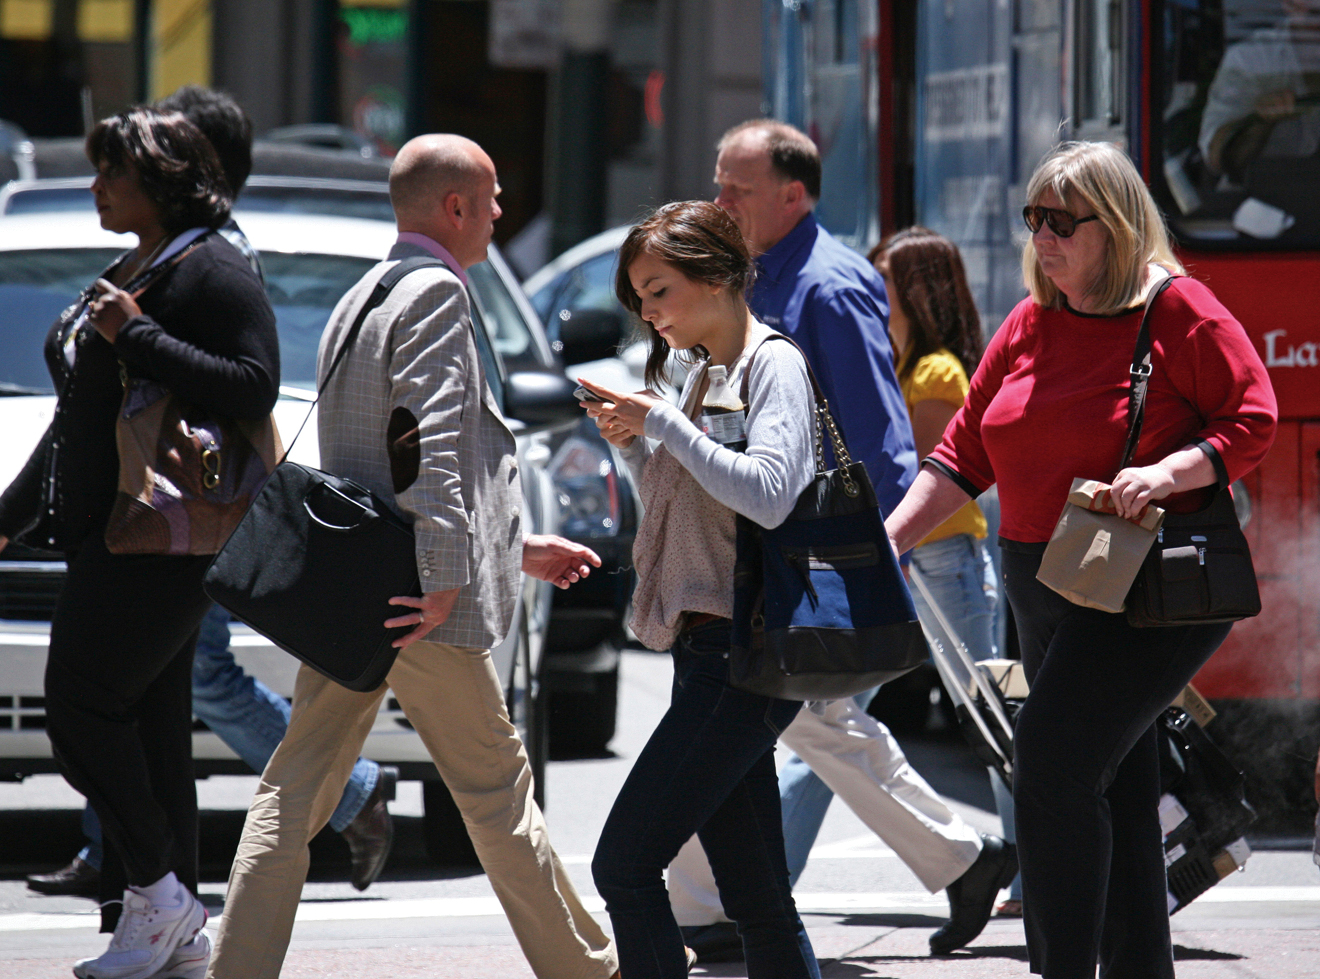
\includegraphics[height=3.9cm]{figures_introduction/pedestrian}}
	\subcaptionbox{\footnotesize Lighting Variation\label{fig:difficult_b}}{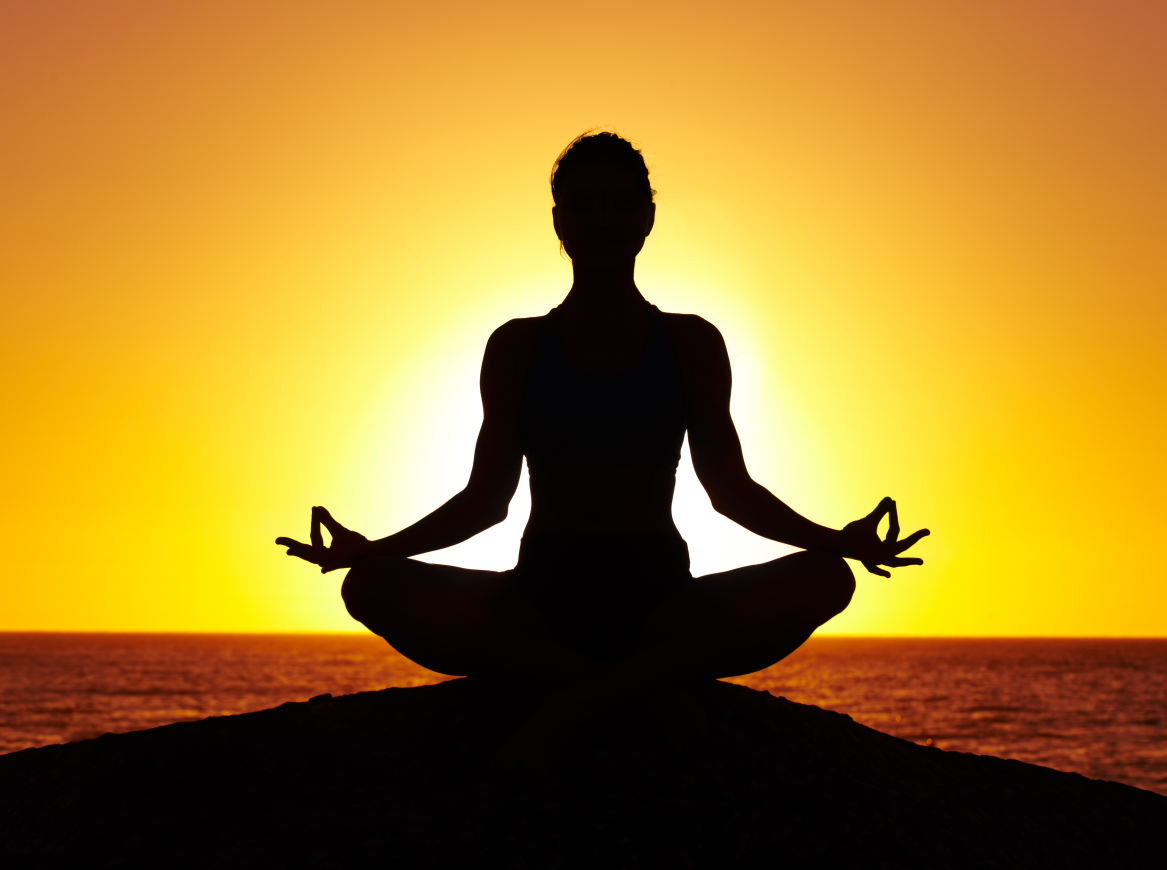
\includegraphics[trim=1.7cm 1.0cm 1.5cm 0.5cm, clip=true, height=3.9cm]{figures_introduction/yoga-pose}}
	\subcaptionbox{\footnotesize Self Occlusion\label{fig:difficult_c}}{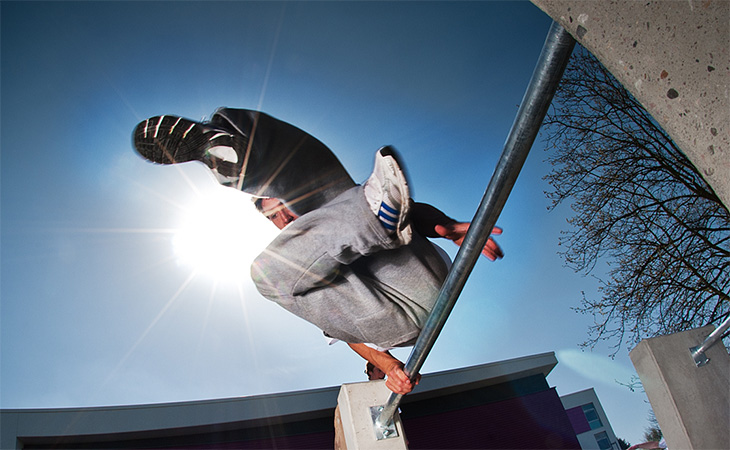
\includegraphics[trim=3.0cm 0.0cm 6.5cm 2.0cm, clip=true, height=3.9cm]{figures_introduction/x-move_parkour_.jpg}}
        \caption{Difficult Samples for Human Body Pose Recognition}
        \label{fig:difficult}
\end{figure}

Human body localization is complicated and difficult for numerous reasons, and some difficult examples are shown in Figure~\ref{fig:difficult}. As with many computer vision applications, the high dimensional nature of the image input makes inferring the low-dimensional pose representation difficult since the input dimensionality cannot be easily enumerated. However, unlike many classic computer vision tasks, human body tracking also involves localizing body parts that undergo large amounts of deformation and exhibit wide variation in both body-shape and appearance. Deformation increases the intrinsic input dimensionality of the space of possible poses and furthermore leads to occlusion, which means that pose inference must be performed with potentially missing data. Appearance variation can be the result of clothing, lighting variation or the subjects age or gender; therefore any inference solution must learn invariance in order to provide a stable estimate of pose under such wildly varying conditions. Lastly, large and comprehensive datasets exist for image classification tasks~\cite{deng2009imagenet}, however human-body pose datasets are many orders of magnitude smaller~\cite{modec,andriluka14cvpr,Johnson10}. The lack of a comprehensive standard dataset has traditionally made training robust discriminative architectures difficult as such networks are prone to over-training when the training set sizes are limited.

Despite these significant challenges, this work will present a framework for human body pose localization that offers a significant improvement over existing traditional architectures. The basis for all the tracking solutions presented in this thesis is the use of Convolutional Networks (ConvNets), which have seen a recent surge in success and popularity due to advances in Graphics Processing Unit (GPU) hardware as well as new and improved techniques for training them. ConvNets are biologically inspired variants of multi-layered perceptrons, which exploit spatial correlation in natural images by extracting features generated by localized convolution kernels. In the context of object detection, the use of fully convolutional networks result in trained detectors which are invariant to translation, and this work makes heavy use of this feature for the architectures presented in Parts \ref{part:two}, \ref{part:three} and \ref{part:four}. A full-review of ConvNets - specifically their formulation and training via the Back-Propagation algorithm - is outside the scope of this thesis and interested readers should refer to \cite{reading_list} for an overview of seminal literature.

ConvNets have been used successfully to solve many difficult machine learning problems: image classification~\cite{pedestrianCVPR13, overfeatSermanet, ImageNet_NIPS2012_0534, googlenet}, scene understanding~\cite{Farabet}, video analysis~\cite{KarpathyCVPR14} and natural language processing~\cite{ilya_sequence,cho_emnlp_2014}. Likewise, they have recently out-performed all existing models on the task of hand-pose recognition~\cite{tompsonTOG14} using an depth camera source, and monocular human-body pose recognition using an RGB camera~\cite{tompsonnips2014, arjunaccv2014, jainiclr2014, deeppose, chennips2014, tompson_efficient}. In this work, we will present our results for the current state-of-the-art models (at time of writing) for human body and hand pose recognition.

\subsection*{Thesis Outline}

This thesis will explore solutions to two difficult computer vision problems related to the localization of humans in images: 1) monocular hand-pose recognition from depth images and 2) monocular full body-pose recognition from RGB images. This exploration will cover four primary publications \cite{tompsonTOG14}, \cite{tompsonnips2014}, \cite{arjunaccv2014}, \cite{tompson_efficient} in Parts \ref{part:one}, \ref{part:two}, \ref{part:three} and \ref{part:four} respectively. Within each part, the first section will define the specific problem and present an overview of the architecture. The second section will present the model and any algorithmic details necessary to repeat experiments. Then the final solution will present experimental results, compare our work with previous state-of-the-art and describe any limitations.

\subsection*{Summary of Contributions}

The following is a summary of the major contributions of this thesis:

\begin{itemize}

\item In Part~\ref{part:one} we describe a novel pipeline for both offline ground truth dataset creation, as well as real-time pose-detection of human hands in depth video. While Neural Networks have been used for pose detection of a limited set of discrete hand gestures (for instance discriminating between a closed fist and an open palm)~\cite{nagi,nowlan}, to our knowledge this is the first work that has attempted to use such networks to perform dense feature extraction of human hands in order to infer continuous pose.

\item In Part~\ref{part:two} we describe a novel ConvNet architecture which combines a traditional sliding-window based part detector with a Graphical Model. We describe a graphical model formulation which is inspired by standard MRF belief propagation, which can be trained jointly with a standard deep-learning architecture to improve detection performance. At the time of writing, this model is the state-of-the-art model for the FLIC~\cite{modec}, LSP~\cite{Johnson10} and MPII~\cite{andriluka14cvpr} datasets.

\item In Part~\ref{part:three} we show that simple motion features can be used to significantly improve the performance of traditional ConvNet architectures. To our knowledge, this was the first work to empirically examine the impact of multi-frame inputs to ConvNets in the application of pose detection.

\item In Part~\ref{part:four} we examine the issue of localization accuracy degradation in ConvNet architecture due to spatial-pooling layers. We present a novel cascaded architecture, that makes use of shared features, in order to improve localization accuracy while maintaining runtime performance. We are the first to show that a ConvNet trained to infer the 2D pose of humans in images is able to be competitive with - and in some cases out-perform - humans trained on the same task.

\end{itemize}
%
%\newpage
\section*{Related Work}\addcontentsline{toc}{chapter}{Related Work}
%%\begin{table} 
\begin{center} 
\begin{tabular}{|c||c|c|c|c|}
\hline
\emph{Algorithm} & \emph{Manifold Model} & \emph{Encode} & \emph{Decode} & \emph{Relate Enc. \& Dec.}\\
%\thickhline
\hline \hline 
\cellcolor{red}PCA & Linear &\checkmark & \checkmark & $W_D = W_E ^T$\\
\hline
\cellcolor{red}ICA & Linear &\checkmark & \checkmark & $W_D = W_E ^T$\\
\hline
\cellcolor{yellow}Sparse Coding & Local Linear &\checkmark & \checkmark & Separate \\
\hline 
\cellcolor{yellow}PSD \& LISTA & Local Linear &\checkmark & \checkmark & Separate\\
\hline
\cellcolor{lightblue}DrLIM & Nonlinear & \checkmark & X & Enc. Only\\
\hline
\cellcolor{lightblue}Chapter \ref{chapter:slow} & Nonlinear & \checkmark & X & Enc. Only\\
\hline
\cellcolor{lightblue}Chapter \ref{chapter:linear} & Nonlinear & \checkmark & \checkmark & Separate\\
\hline
Adversarial Networks & Nonlinear & X & \checkmark & Dec. Only \\
\hline 
\cellcolor{green}Auto-Encoders & Nonlinear & \checkmark & \checkmark & Separate \\
\hline 
\end{tabular} \\
\vspace{0.25cm} \hspace{0.25cm}  
\begin{tabular}{|c|}
\hline 
\emph{Model Objective/Prior}\\  
\hline \hline
\cellcolor{red} De-correlation/Independence  \\
\hline
\cellcolor{yellow} Sparsity \\
\hline
\cellcolor{lightblue} Metric Learning/Geometric Prior  \\
\hline
\cellcolor{green} All of the Above \\
\hline
None \\
\hline
\end{tabular}
\end{center}
\caption{Summary of unsupervised feature learning algorithms and their properties} 
\label{tbl:models} 
\end{table} 

Unsupervised feature learning arguably dates back to the invention of Principal
Component Analysis (PCA) in 1901 by Karl Pearson \cite{PCA}. As mentioned in
Chapter \ref{chapter:introduction}, feature learning algorithms model
intrinsically low dimensional data embedded in a high dimensional ambient
space. These models can usually be decomposed into two parts: a mapping from
the input space to the feature space, called encoding, and mapping the feature
space back to the input space, called decoding. If the encoding or decoding
processes have corresponding functional forms, they are referred to as the
``encoder'' and ``decoder'', respectively.  From the natural image manifold
perspective, ideal encodings map the extrinsic coordinates (i.e. pixel values)
to intrinsic manifold coordinates. It is hoped that these intrinsic coordinates
correspond to physical attributes of the natural world, such as the presence of
certain objects in the scene, their properties, etc \cite{nair2008,capsules}.
Unsupervised feature learning models are mainly distinguished by: i-the
geometrical prior they assume about the data manifold, ii-whether they learn an
encoder, decoder, or both. For example, Principal Component Analysis assumes
that the data is concentrated around a hyper-plane, i.e. it assumes a globally
linear data manifold model. The PCA encoder is a matrix operator, $W_e$, as is
the decoder $W_d=W_e^T$.  Obtaining ``invariant'' representations has been a
major driving force in feature learning, driven mainly by recognition and
classification problems.  Invariant features imply that the encoding process is
necessarily a many-to-one mapping. This means that the decoding process must
involve some random selection among the possible inputs that produced the code,
usually  by sampling from a distribution. Models that include a decoder are
called ``generative models'' in the literature. 

Table \ref{tbl:models} summarizes key aspects of several well-known feature
learning models, as well as the new models which will be introduced in Chapters
\ref{chapter:slow} and \ref{chapter:linear}. The first column lists the name of
the model, the color indicates the type of objective each model tries to
optimize.  These are summarized in the table below. For example, one version of
PCA finds maximally decorrelated linear components. The ``manifold model''
column indicates the geometric prior each model assumes about the data
manifold. The next two columns indicate whether each model learns an encoder
and/or decoder.  Finally, the last column summarizes the relationship enforced
between the encoder and decoder. For example in PCA the encoder and decoder are
related by the transpose operator. This chapter will review the algorithms in
Table \ref{tbl:models}, placing emphasis on the precursors of the algorithms
presented in Chapters \ref{chapter:slow} and \ref{chapter:linear}. The
algorithms will be presented as various models of the data manifold.

\section{Principal and Independent Component Analysis} 

\begin{figure} 
\centering
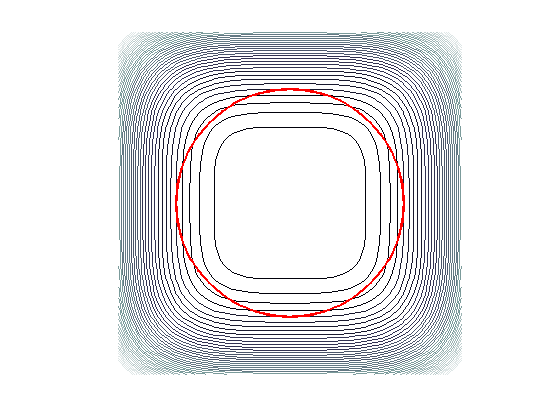
\includegraphics[scale=0.4]{./figures/related_work/ICA.png} 
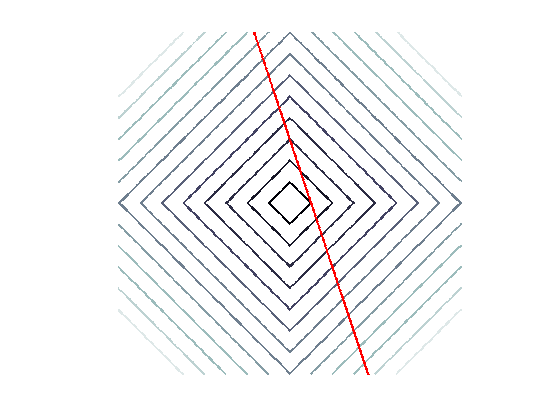
\includegraphics[scale=0.4]{./figures/related_work/L1.png} 
\caption{Left: visualization of the optimization problem used to solve for independent representations. Right: visualization of the optimization problem used to solve for sparse representations.} 
\label{fig:ICA_lasso} 
\end{figure}  

Principal Component Analysis (PCA) and Independent Component Analysis (ICA) are
the most well know linear manifold models \cite{ICA}. Both assume that the
observed high dimensional data $x$ are generated from some low dimensional
latent variables $z$ via a linear operator $A$, that is $x=Az$. Assuming that
the data is zero mean, PCA implicitly makes the assumption that the latent
variables correspond to directions with the largest variance \cite{PCA}.  These
components can be obtained from the Eigen decomposition of the covariance
matrix.  ICA however searches for linearly independent components, formulating
the definition of independence using the central limit theorem. Although the
detailed derivation of ICA will not be presented here, we will mention that it
leads to a fourth order moment (kurtosis) maximization problem subject to a
second order moment (variance) constraint. This optimization problem is
visualized as the left plot of Figure \ref{fig:ICA_lasso}. The blue curves
represent the level sets of the kurtosis objective, and the red curve
represents the unit variance constraint. The next section will establish a 
remarkable connection between ICA and sparse inference.  

\section{Sparse Representations} 
Sparse inference refers to the problem of finding the coefficients $z$ which
reconstruct the input $x$ as a sparse linear combination of some basis elements
contained an over-complete dictionary $W_d$. Sparsity is measured by the number
of non-zero coefficients; the higher the sparsity the fewer non-zero
coefficients in $z$ used to represent $x$.  
The sparse inference problem can be stated formally as: 

\begin{equation} 
min \|z\|_0 \mbox{ subject to } x = W_dz 
\end{equation} 

In general, this is an intractable combinatorial problem. A now famous
breakthrough showed that exact sparse solutions can be obtained, under certain
conditions, by replacing the $L_0$ norm with an $L_1$ norm \cite{candes2006}.
This optimization problem is depicted on the right side of Figure
\ref{fig:ICA_lasso}.  The level sets of the $L_1$ norm are shown in blue and
the linear constraint is shown in red. The minimum occur on the $x$-axis, with
$y=0$ implying that the solution is indeed sparse. Remarkably, the solution to
the ICA problem (left side of Figure \ref{fig:ICA_Lasso}) is also sparse though the
objective was explicitly derived with sparsity in mind.    

Relaxing the constraint, this problem can be written as an unconstrained loss
functional called the lasso (also basis pursuit de-noising) \cite{BP}:  

\begin{equation} 
L_{lasso} = \frac{1}{2}\|x-W_dz\| + \alpha |z|_1
\end{equation} 


\section{Metric Learning}

\section{Auto-Encoders and Energy Based Learning} 
 

%
\part{Regularized Auto-Encoders and Dictionary Learning}
\label{part:one}
%%\chapter{Overview\label{chap:1_hand_tracking_overview}}

In this Part we present a solution to the difficult problem of inferring the continuous pose of a human hand. We do so by first constructing an accurate database of labeled ground-truth data in an automatic process, and then training a system capable of real-time inference using ConvNets. Since the human hand represents a particularly difficult kind of articulable object to track, we believe our solution is applicable to a wide range of articulable objects. Our method has a small latency equal to one frame of video, is robust to self-occlusion, requires no special markers, and can handle objects with self-similar parts (i.e. fingers). To allow a broad range of applications, our method works when the hand is smaller than 2\% of the $640\times480$px image area.

Traditionally, commercial motion capture solutions have not included infrastructure to infer hand pose and instead focus on full-body skeletal animation. This is largely due to the difficulty that arises because articulable objects - like the human hand - have many DOF, constrained parameter spaces, self-similar parts, and suffer from self-occlusion. For this work we utilize a depth camera since it provides a dense set of accurate measurements of the physical geometry of the hand, however even with this high dimensional input modality, inferring the pose is still difficult because of data loss due to ``dropped-pixels'' (an artifact of the depth sensing device) and self occlusion.

One common approach to ``fill in'' missing data is to combine multiple simultaneous video streams; but this is a costly demand on the end-user and may prohibit widespread use of otherwise good solutions. A second common approach, called ``supervised learning'' in computer vision and machine learning, is to train a model on ground-truth data, which combines the full pose of the object in the frame with the depth image. The trained model can then use a priori information from known poses to make informed guesses about the likely pose in the current frame.

Large ground-truth datasets have been constructed for important articulable objects such as human bodies. Unfortunately, most articulable objects, even common ones such as human hands, do not have publicly available datasets, or these datasets do not adequately cover the vast range of possible poses. Perhaps more importantly, it may be desirable to infer the real-time continuous pose of objects that do not yet have such datasets. The vast majority of objects seen in the world fall into this category, and a general method for dataset acquisition of articulable objects is an important contribution of this work.

The main difficulty with using supervised learning for training models to perform real-time pose inference of a human hand is in obtaining ground-truth data for hand pose. Typical models of the human hand have 25-50 degrees of freedom ~\cite{erol2007vision} and exclude important information such as joint angle constraints. Since real hands exhibit joint angle constraints that are pose dependent, faithfully expressing such limits is still difficult in practice. Unfortunately, without such constraints, most models are capable of poses which are anatomically incorrect. This means that sampling the space of possible parameters using a real hand is more desirable than exploring it with a model. With the advent of commodity depth sensors, it is possible to economically capture continuous traversals of this constrained low-dimensional parameter space in video, and then robustly fit hand models to the data to recover the pose parameters~\cite{bmvc2011oikonom}.

\begin{figure}[ht]
\centering
\includegraphics[width=0.8\columnwidth]{figures_1_hand_tracking/overview.pdf}
    \caption{Pose Recovery Pipeline Overview}
    \label{fig:overview}
\end{figure}

Our method can be generalized to track any articulable object that satisfies three requirements: 1) the object to be tracked can be modeled as a 3D boned mesh, 2) a binary classifier can be made to label the pixels in the image belonging to the object, and 3) the projection from pose space (of the bones) to a projected 2D image in depth is approximately one-to-one. 

An overview of this pipeline is shown in Figure~\ref{fig:overview} and the output of each stage is shown in Figure~\ref{fig:overview_detail}. The 3D boned mesh of the articulable object is used to automatically label depth video captured live from a user. This data is used to train a Randomized Decision Forest (RDF) architecture for image segmentation (output shown in Figure~\ref{fig:overview_detail_a}), create a comprehensive database of depth images with ground-truth pose labels (output shown in Figure~\ref{fig:overview_detail_b}), which is then used to train a ConvNet to infer the position of key model features in real-time (output shown in Figure~\ref{fig:overview_detail_c}). We also suggest a simple and robust inverse kinematics (IK) algorithm for real-time, high degree of freedom pose inference from the ConvNet output (output shown in Figure~\ref{fig:overview_detail_d}). 

Note that our system can accommodate multiple commodity depth cameras for generating training data, but requires only a single depth camera for real-time tracking.

\begin{figure}[ht]
\centering
        % trim option's parameter order: left bottom right top
	\subcaptionbox{\footnotesize RDF classification\label{fig:overview_detail_a}}{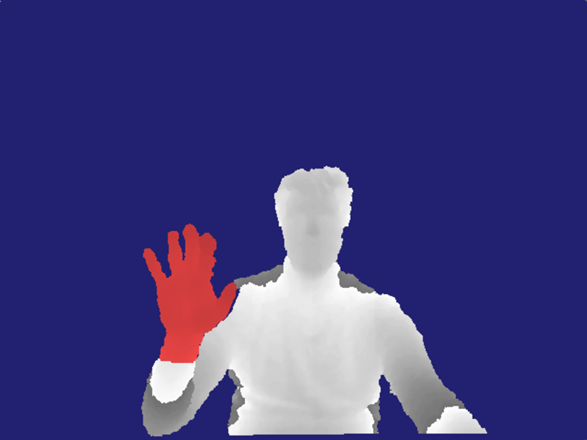
\includegraphics[height=3.7cm, trim = 20mm 0mm 30mm 22.5mm, clip]{figures_1_hand_tracking/overview_1}}
	\subcaptionbox{\footnotesize Model Fitting\label{fig:overview_detail_b}}{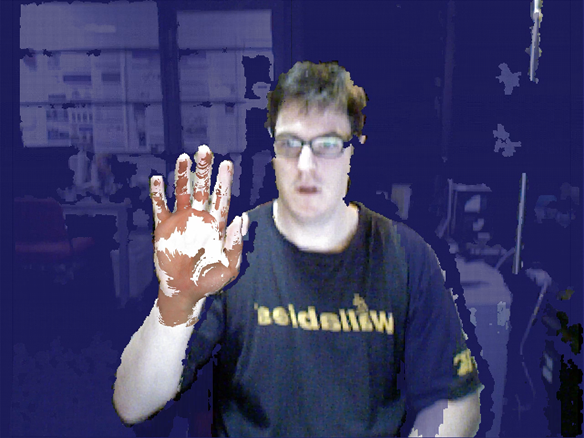
\includegraphics[height=3.7cm, trim = 15mm 0mm 20mm 5mm, clip]{figures_1_hand_tracking/overview_2}}
        \subcaptionbox{\footnotesize ConvNet Inference\label{fig:overview_detail_c}}{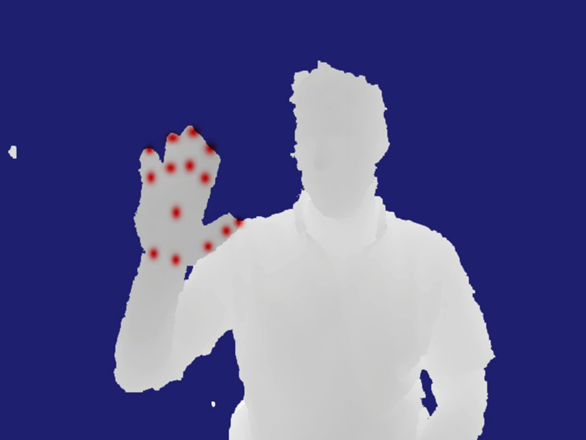
\includegraphics[height=3.7cm, trim = 15mm 0mm 20mm 5mm, clip]{figures_1_hand_tracking/overview_3}}
        \subcaptionbox{\footnotesize IK\label{fig:overview_detail_d}}{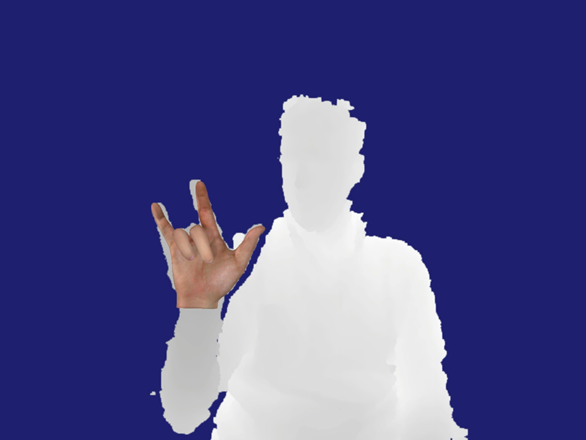
\includegraphics[height=3.7cm, trim = 20mm 0mm 15mm 10mm, clip]{figures_1_hand_tracking/overview_4}}
        \caption{Pipeline Stage Outputs}
        \label{fig:overview_detail}
\end{figure}

As a single example, training our system on an open-source linear-blend-skinning model of a hand with 42 degrees of freedom takes less than 10 minutes of human effort (18,000 frames at 30fps), followed by two days of autonomous computation time. Tracking and pose inference for a person's hand can then be performed in real-time using a single depth camera. Throughout our experiments, the camera is situated in front of the user at approximately eye-level height. The trained system can be readily used to puppeteer related objects such as alien hands, or real robot linkages, and as an input to 3D user interfaces~\cite{Stein2012}.

\chapter{Hand Tracking Architecture\label{chap:1_hand_tracking_archiecture}}

\section{Binary Classification}
\label{sec:binary_classification}

For the task of hand-background depth image segmentation we trained an RDF classifier to perform per-pixel binary segmentation on a single image. The output of this stage is shown in Figure \ref{fig:rdf_data}. Decision forests are well-suited for discrete classification of body parts~\cite{shotton2013real}. Furthermore, since decision forest classification is trivially parallelizable, it is well-suited to real-time processing in multi-core environments.

\begin{figure}[ht]
\centering
        \begin{subfigure}{0.4\textwidth}
                \centering
                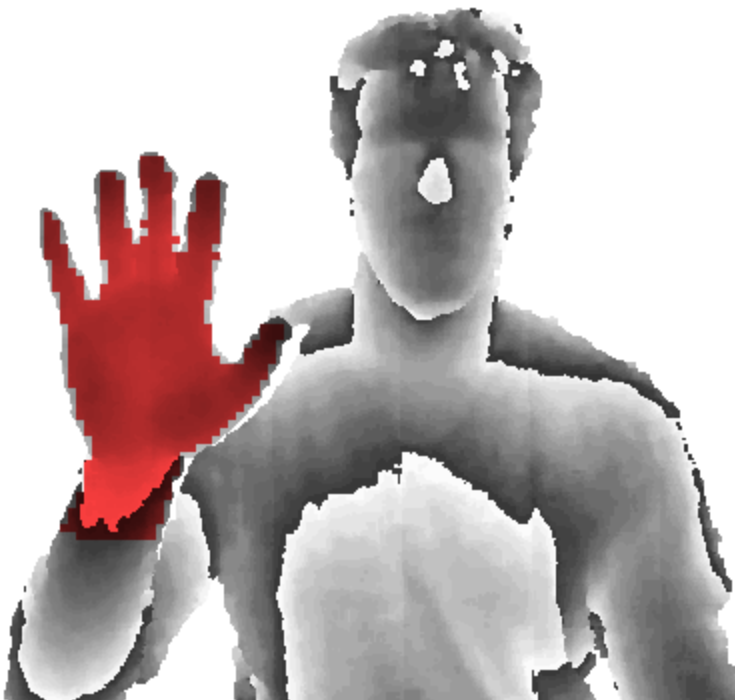
\includegraphics[width=\textwidth]{figures_1_hand_tracking/decision_forest_downsampled_labels_cropped}
                \caption{\footnotesize Ground-Truth Labels}
        \end{subfigure}
        \begin{subfigure}{0.4\textwidth}
                \centering
                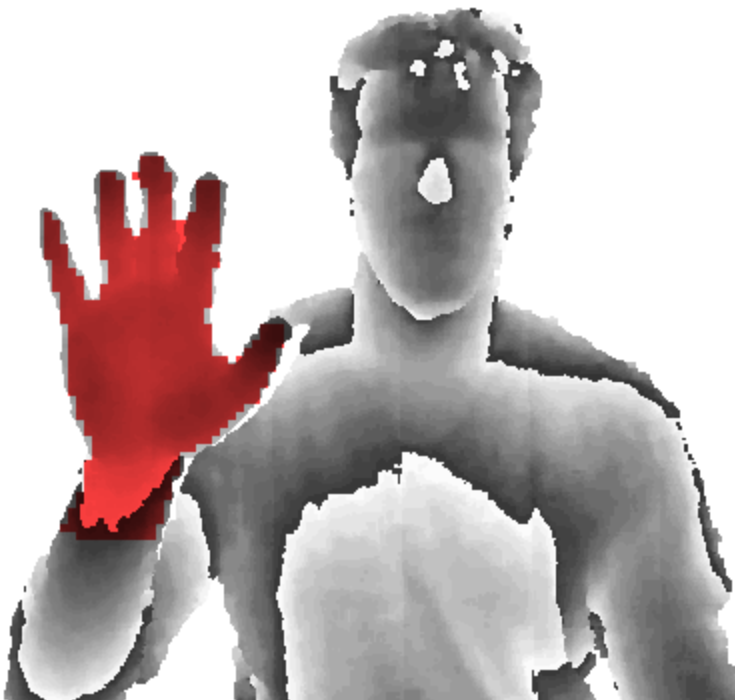
\includegraphics[width=\textwidth]{figures_1_hand_tracking/decision_forest_generated_labels_cropped}
                \caption{\footnotesize Labels Inferred by RDF}
        \end{subfigure}
        \caption{Decision Forest Data: learned labels closely match target}
        \label{fig:rdf_data}
\end{figure}

After Shotton et al., our RDF is designed to classify each pixel in a depth image as belonging to a hand or background. Each tree in the RDF consists of a set of sequential deterministic decisions, called weak-learners (or nodes), that compare the relative depth of the current pixel to a nearby pixel located at a learned offset. The particular sequence of decisions a pixel satisfies induces a tentative classification into hand or background. An overview of the RDF architecture is shown in Figure~\ref{fig:rdf_overview}. For each pixel in the image, the algorithm starts at the root of each Randomized Decision Tree (RDT) and proceeds down the left or right sub-trees according to the binary decision made by the weak-learner at each node.  The leaf nodes describe the distribution of labels in the training set for the pixels that satisfy the weak-learner sequence. Averaging the classification from all trees in the forest induces a final probability distribution for each pixel, where the inferred label is taken as the argmax of the distribution. As our implementation differs only slightly from that of Shotton et al., we refer interested readers to their past work, and focus on the innovations particular to our implementation.

\begin{figure}[ht]
\centering
\includegraphics[width=0.8\columnwidth]{figures_1_hand_tracking/RDF}
    \caption{RDF Overview}
    \label{fig:rdf_overview}
\end{figure}

While full body motion capture datasets are readily available~\cite{Allen2003}, these datasets either lack articulation data for hands or else do not adequately cover the wide variety of poses that were planned for this system. Therefore, it was necessary to create a custom database of full body depth images with binary hand labeling for RDF training (Figure \ref{fig:rdf_data}). We had one user paint their hands bright red with body paint and used a simple HSV-based distance metric to estimate a coarse hand labeling on the RGB image. The coarse labeling is then filtered using a median filter to remove outliers. Since commodity RGB+Depth (RGBD) cameras, typically exhibit imperfect alignment between depth and RGB, we used a combination of graph cut and depth-sensitive flood fill to further clean up the depth image labeling~\cite{Boykov}.

In order to train the RDF we randomly sample weak-learners from a family of functions similar to \cite{shotton2013real}. At a given pixel $(u,v)$ on the depth image $I$ each node in the decision tree evaluates:
\begin{equation}
    I\left(u + \frac{\Delta u}{I\left(u,v\right)}, v + \frac{\Delta v}{I\left(u,v\right)}\right) - I\left(u,v\right)\geq d_{t}
    \label{eq:rdf}
\end{equation}
Where $I\left(u,v\right)$ is the depth pixel value in image $I$, $\Delta u$ and $\Delta v$ are learned pixel offsets, and $d_{t}$ is a learned depth threshold. Experimentally, we found that (\ref{eq:rdf}) requires a large dynamic range of pixel offsets during training to achieve good classification performance. We suspect that this is because a given decision path needs to use both global and local geometry information to perform efficient hand-background segmentation. Since training time is limited, we define a discrete set of weak-learners that use offset and threshold values that are linear in log space and then we randomly sample weak-learners from this space during training.

\section{Dataset Creation}
\label{sec:datasetcreation}

The goal of this stage is to create a database of RGBD sensor images representing a broad range of hand gestures with accurate ground-truth estimates (i.e. labels) of joint parameters in each image that may be used to train a ConvNet. The desired ground-truth label consists of a 42-dimensional vector describing the full degree of freedom pose for the hand in that frame. The DOF of each hand-joint is shown in Figure \ref{fig:libhand}. After the hand has been segmented from the background using the RDF-based binary classification just described, we use a direct search method to deduce the pose parameters based on the approach of Oikonomidis et al.~\cite{bmvc2011oikonom}. An important insight of our work is that we can capture the power of their direct search method in an offline fashion, and then use it to train ConvNets (or similar  algorithms) that are better suited to fast computation. One advantage of this decoupling is that during offline training we are not penalized for using more complicated models, which are more expensive to render, and which better explain the incoming range data. A second advantage is that we can utilize multiple sensors for training, thereby mitigating problems of self-occlusion during real-time interaction with a single sensor.

\begin{figure}[ht]
\centering
\includegraphics[width=0.4\textwidth]{figures_1_hand_tracking/libhand.pdf}
    \caption{Linear Blend Skinning (LBS) Model~\protect\cite{libhand} with 42 DOF}
    \label{fig:libhand}
\end{figure}

The algorithm proposed by Oikonomidis et al.~\cite{bmvc2011oikonom} and adopted with modifications for this work is as follows; starting with an approximate hand pose, a synthetic depth image is rendered and compared to the depth image using an scalar objective function. This depth image is rendered in an OpenGL-based framework, where the only render output is the distance from the camera origin and we use a camera with the same properties (e.g. focal length) as the PrimeSense IR sensor. In practice the hand pose is estimated using the previous frame's pose when fitting a sequence of recorded frames. The pose is manually estimated using a simple UI for the first frame in a sequence. This results in a single scalar value representing the quality of the fit given the estimated pose coefficients. The particle swarm optimization with partial randomization (PrPSO) direct search method~\cite{PRPSO} is used to adjust the pose coefficient values to find the best fit pose that minimizes this objective function value. An overview of this algorithm is shown in Figure \ref{fig:pso_architecture}.

\begin{figure}[ht]
\centering
\includegraphics[width=0.6\textwidth]{figures_1_hand_tracking/dataset_generation.pdf}
    \caption{Algorithm Pipeline For Dataset Creation}
    \label{fig:pso_architecture}
\end{figure}

Since PSO convergence is slow once the swarm positions are close to the final solution (which is exacerbated when partial randomization is used to prevent premature swarm collapse on early local minima), we then use a robust variant of the Nelder-Mead optimization algorithm~\cite{Tseng95fortified-descentsimplicial} after PSO has completed. The Nelder-Mead optimization algorithm is a simplex-based direct-search optimization algorithm for non-linear functions. We have found that for our optimization problem, it provides fast convergence when sufficiently close to local optima.

Since this dataset creation stage is performed offline, we do not require it to be fast enough for interactive frame rates. Therefore we used a high-quality, linear-blend-skinning (LBS) model~\cite{libhand} (shown in Figure \ref{fig:libhand}) as an alternative to the simple ball-and-cylinder model of Oikonomidis et al. After reducing the LBS model's face count to increase render throughput, the model contains 1,722 vertices and 3,381 triangle faces, whereas the high density source model contained 67,606 faces. While LBS fails to accurately model effects such as muscle deformation and skin folding, it represents many geometric details that ball-and-stick models cannot.

To mitigate the effects of self-occlusion we used three sensors (at viewpoints separated by approximately 45 degrees surrounding the user from the front), with attached vibration motors to reduce IR-pattern interference~\cite{shake_n_sense} and whose relative positions and orientations were calibrated using a variant of the Iterative Closest Point (ICP) algorithm~\cite{Horn87closed-formsolution}. While we use all three camera views to fit the LBS model using the algorithm described above, we only use depth images taken from the center camera to train the ConvNet. The contributions from each camera were accumulated into an overall fitness function $F\left(C\right)$, which includes two \emph{a priori} terms ($\Phi\left(C\right)$ and $P\left(C\right)$) to maintain anatomically correct joint angles as well as a data-dependent term $\Delta(I_s, C)$ from each camera's contribution. The fitness function is as follows:

\begin{equation}
    F\left(C\right)=\sum_{s=1}^3\bigg(\Delta(I_s, C)\bigg) + \Phi\left(C\right) + P\left(C\right)
    \label{eq:pso_func}
\end{equation}

Where $I_s$ is the $s$ sensor's depth image and $C$ is a 42-dimensional coefficient vector that represents the 6 DOF position and orientation of the hand as well as 36 internal joint angles (shown in Figure \ref{fig:libhand}). $P\left(C\right)$ is an interpenetration term (for a given pose) used to invalidate anatomically incorrect hand poses and is calculated by accumulating the interpenetration distances of a series of bounding spheres attached to the bones of the 3D model. We define interpenetration distance as simply the sum of overlap between all pairs of interpenetrating bounding spheres. $\Phi\left(C\right)$ enforces a soft constraint that coefficient values stay within a predetermined range ($C_{\text{min}}$ and $C_{\text{max}}$):

\begin{equation*}
    \Phi\left(C\right) = \sum\limits_{k=1}^n w_k\left[\operatorname{max}\left(C_k-C_{k\text{max}}, 0\right) + \operatorname{max}\left(C_{k\text{min}}-C_k, 0\right)\right]
    \label{eq:pso_penalty}
\end{equation*}

Where, $w_k$ is a per-coefficient weighting term to normalize penalty contributions across different units (since we are including error terms for angle and distance in the same objective function). $C_{\text{min}}$ and $C_{\text{max}}$ were determined experimentally by fitting an unconstrained model to a discrete set of poses which represent the full range of motion for each joint. Lastly $\Delta(I_s, C)$ of Equation (\ref{eq:pso_func}), measures the similarity between the depth image $I_s$ and the synthetic pose rendered from the same viewpoint:

\[
    \Delta\left(I_s,C\right)=\sum_{u,v}\operatorname{min}\left(\left|I_s(u,v)-R_s(C,u,v)\right|,d_{\text{max}}\right)
    \label{eq:pso_depth_compare}
\]

Where, $I_s(u,v)$ is the depth at pixel $(u,v)$ of sensor $s$, $R_s(C,u,v)$ is the synthetic depth given the pose coefficient C and $d_{\text{max}}$ is a maximum depth constant. The result of this function is a clamped L1-norm pixel-wise comparison. It should be noted that we do not include energy terms that measure the silhouette similarity as proposed by Oikonomidis et al. since we found that when multiple range sensors are used these terms are not necessary.

Since the same pose is seen by multiple cameras from different viewpoints, it is necessary to calculate an affine transformation from each camera's viewpoint into a consistent basis. Due to variations in the imaging systems of each camera, small three-dimensional scale variations are common across views of the same object. For this reason, classical iterative closest point (ICP) with scale ~\cite{Horn87closed-formsolution} is insufficient for our needs, and instead we use a straightforward weighted variant of ICP based on energy minimization. In this variant, for an arbitrary 3D point in the data $p_j$, and the corresponding closest point $q_j$ on the model, we minimize the overall discrepancy of the fit $E$, given the current camera to world coordinate transformation $T_i$ (for each camera $i$), as follows:

\begin{align}
E = \sum_{i=1}^N\sum_{j=1}^Mw_j\left\|T_iq_j - p_j\right\|^2 \nonumber \\
w_j = \frac{\operatorname{max}\left(0, \frac{\text{dot}(\hat{q_j}, \hat{p_j}) - k}{ 1 - k}\right)}{1 + \left\|p_j-q_j\right\|} \nonumber
\end{align}

Where there are $N+1$ cameras and $M$ points in our system. The per-correspondence weight $w_j$ biases the fit towards points that are already close and have normals $\hat{p_j},\hat{q_j}$ pointing in the same direction. The resulting fit is mostly insensitive to the constant $k \in (0,1)$, and we used $k = 0.5$. Using suitable calibration geometry and a known approximate initial transformation, the above algorithm converges within 50 to 100 iterations using BFGS to perturb the parameters of the affine matrices $T_i$.

\section{Feature Detection}
\label{sec:realtimefeaturedetection}

We employ a multi-resolution, deep ConvNet architecture inspired by the work of Farabet et al.~\cite{Farabet} in order to perform feature extraction of 14 salient hand points from a segmented hand image. Since depth images of hands tend to have many repeated local image features (for instance fingertips), ConvNets are well suited to perform feature extraction since multi-layered feature banks can share common features, thereby reducing the number of required free parameters.

We recast the full hand-pose recognition problem as an intermediate collection of easier individual hand-feature recognition problems, which can be more easily learned by ConvNets. In early experiments we found inferring mappings between depth image space and pose space directly (for instance measuring depth image geometry to extract a joint angle), yielded inferior results to learning with intermediate features. We hypothesize that one reason for this could be that learning intermediate features allows ConvNets to concentrate the capacity of the network on learning local features, and on differentiating between them. Using this framework the ConvNet is also better able to implicitly handle occlusions; by learning compound, high-level image features the ConvNet is able to infer the approximate position of an occluded and otherwise unseen feature (for instance, when making a fist, hidden finger-tip locations can be inferred by the knuckle locations).

We trained the ConvNet architecture to generate an output set of \emph{heat-map} feature images (Figure \ref{fig:heat_maps}). Each feature heat-map can be viewed as a 2D Gaussian (truncated to have finite support), where the pixel intensity represents the probability of that feature occurring in that spatial location. The Gaussian UV mean is centered at one of 14 feature points of the user's hand. These features represent key joint locations in the 3D model (e.g., knuckles) and were chosen such that the inverse kinematics (IK) algorithm described in Section \ref{sec:realtimeposedetection} can recover a full 3D pose.

\begin{figure}[ht]
\centering
\includegraphics[width=\textwidth]{figures_1_hand_tracking/heat_maps_2_feat.pdf}
    \caption{Depth image overlaid with 14 feature locations and the heat-map for two fingertip features.}
    \label{fig:heat_maps}
\end{figure}

We found that the intermediate heat-map representation not only reduces required learning capacity but also improves generalization performance since failure modes are often recoverable. Cases contributing to high test set error (where the input pose is vastly different from anything in the training set) are usually heat-maps that contain multiple hotspots. For instance, the heat-map for a fingertip feature might incorrectly contain multiple lobes corresponding to the other finger locations as the network failed to discriminate among fingers. When this situation occurs it is possible to recover a reasonable feature location by simple heuristics to decide which of these lobes corresponds to the desired feature (for instance if another heat-map shows higher probability in those same lobe regions then we can eliminate these as spurious outliers). Similarly, the intensity of the heat-map lobe gives a direct indication of the system's confidence for that feature, which is an extremely useful measure for practical applications.

Our multi-resolution ConvNet architecture is shown in Figure \ref{fig:cnn}. The segmented depth image is initially pre-processed, whereby the image is cropped and scaled by a factor proportional to the mean depth value of the hand pixels, so that the hand is in the center and has size that is depth invariant. The depth values of each pixel are then normalized between 0 and 1 (with background pixels set to 1). The cropped and normalized image is shown in Figure \ref{fig:heat_maps}.

\begin{figure}[ht]
\centering
\includegraphics[width=0.9\textwidth]{figures_1_hand_tracking/CNN_architecture.pdf}
    \caption{Convolutional Network Architecture}
    \label{fig:cnn}
\end{figure}

The preprocessed image is then filtered using local contrast normalization~\cite{JarrettLeCun}, which acts as a high-pass filter to emphasize geometric discontinuities. The image is then down-sampled twice (each time by a factor of 2) and the same filter is applied to each image. This produces a multi-resolution band-pass image pyramid with 3 banks (shown in Figure \ref{fig:pyramid}), whose total spectral density approximates the spectral density of the input depth image. Since experimentally we have found that hand-pose extraction requires knowledge of both local and global features, a single resolution ConvNet would need to examine a large image window and thus would require a large learning capacity; as such a multi-resolution architecture is very useful for this application.

\begin{figure}[ht]
\centering
        \begin{subfigure}{0.3\textwidth}
                \centering
                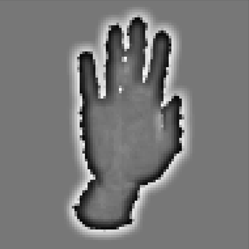
\includegraphics[width=\textwidth]{figures_1_hand_tracking/pyramid1}
                \caption{\footnotesize 96$\times$96px}
        \end{subfigure}
        \begin{subfigure}{0.3\textwidth}
                \centering
                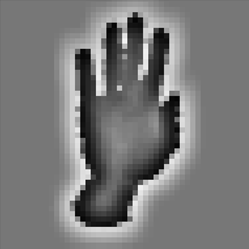
\includegraphics[width=\textwidth]{figures_1_hand_tracking/pyramid2}
                \caption{\footnotesize 48$\times$48px}
        \end{subfigure}
        \begin{subfigure}{0.3\textwidth}
                \centering
                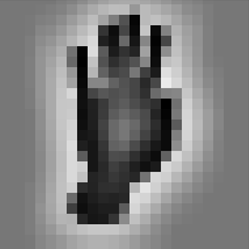
\includegraphics[width=\textwidth]{figures_1_hand_tracking/pyramid3}
                \caption{\footnotesize 24$\times$24px}
        \end{subfigure}
        \caption{Neural Network Input: Multi-Resolution Image Pyramid}
        \label{fig:pyramid}
\end{figure}

The pyramid images are propagated through a 2-stage ConvNet architecture. The highest resolution feature bank is shown in Figure \ref{fig:feature_detector}. Each bank is comprised of 2 convolution modules, 2 piecewise non-linearity modules, and 2 max-pooling modules. Each convolution module uses a stack of learned convolution kernels with an additional learned output bias to create a set of output feature maps (please refer to \cite{LeCunMNIST} for an in-depth discussion). The convolution window sizes range from 4x4 to 6x6 pixels. Each max-pooling~\cite{nagi} module sub-samples it's input image by taking the maximum in a set of non-overlapping rectangular windows. We use max-pooling since it effectively reduces computational complexity at the cost of spatial precision. The max-pooling windows range from 2x2 to 4x4 pixels. The nonlinearity is a Rectify Linear Unit (ReLU), which has been shown to improve training speed and discrimination performance in comparison to the standard sigmoid units~\cite{ImageNet_NIPS2012_0534}. Each ReLU activation module computes the following per-pixel non-linear function:

\begin{equation*}
    f\left(x\right)=\operatorname{max}\left(0,x\right)
\end{equation*}

\begin{figure}[ht]
\centering
\includegraphics[width=0.85\textwidth]{figures_1_hand_tracking/feature_detector.pdf}
    \caption{High-Resolution Bank Feature Detector: (each stage: Nfeats,height,width)}
    \label{fig:feature_detector}
\end{figure}

Lastly, the output of the ConvNet banks are fed into a 2-stage neural network shown in Figure \ref{fig:linear_network}. This network uses the high-level convolution features to create the final 14 heat-map images; it does so by learning a mapping from localized convolution feature activations to probability maps for each of the bone features. In practice these two large and fully-connected linear networks account for more than 80\% of the total computational cost of the ConvNet. However, reducing the size of the network has a very strong impact on runtime performance. For this reason, it is important to find a good tradeoff between quality and speed. Another drawback of this method is that the neural network must implicitly learn a likelihood model for joint positions in order to infer anatomically correct output joints. Since we do not explicitly model joint connectivity in the network structure, the network requires a large amount of training data to perform this inference correctly.

\begin{figure}[ht]
\centering
\includegraphics[width=0.65\textwidth]{figures_1_hand_tracking/linear_network.pdf}
    \caption{2-Stage Neural Network To Create The 14 Heat Maps (with sizing of each stage shown)}
    \label{fig:linear_network}
\end{figure}

ConvNet training was performed using the open-source machine learning package Torch7~\cite{torch7}, which provides access to an efficient GPU implementation of the back-propagation algorithm for training neural networks. During supervised training we use stochastic gradient descent with a standard L2-norm error function, batch size of $64$ and the following learnable parameter update rule:

\begin{align}
    %\gamma_i = \operatorname{max}\left(\gamma_{min},\gamma_0-k\left(i-1\right)\right) \nonumber \\
    \Delta w_i = \gamma\Delta w_{i-1}-\lambda\left(\eta w_i-\frac{\partial L}{\partial w_i}\right) \nonumber \\
    w_{i+1} = w_i + \Delta w_i
\end{align}

Where $w_i$ is a bias or weight parameter for each of the network modules for epoch $i$ (with each epoch representing one pass over the entire training-set) and $\frac{\partial L}{\partial w_i}$ is the partial derivative of the error function $L$ with respect to the learnable parameter $w_i$ averaged over the current batch. We use a constant learning rate of $\lambda = 0.2$, and a momentum term $\gamma=0.9$ to improve learning rate when close to the local minimum. Lastly, an L2 regularization factor of $\eta=0.0005$ is used to help improve generalization.

During ConvNet training the pre-processed database images were randomly rotated, scaled and translated to improve generalization performance~\cite{Farabet}. Not only does this technique effectively increase the size of the training set (which improves test / validation set error), it also helps improve performance for other users whose hand size is not well represented in the original training set. We perform this image manipulation in a background thread during batch-training so the impact on training time is minimal.

\section{Pose Recovery}
\label{sec:realtimeposedetection}

We formulate the problem of pose estimation from the heat-map output as an optimization problem, similar to inverse kinematics (IK). We extract 2D and 3D feature positions from the 14 heat-maps and then minimize an appropriate objective function to align 3D model features to each heat-map position.

To infer the 3D position corresponding to a heat-map image, we need to determine the most likely UV position of the feature in the heat-map. Although the ConvNet architecture is trained to output heat-map images of 2D Gaussians with low-variance, in general, they output multimodal grayscale heat-maps which usually do not sum to 1. In practice, it is easy to deduce a correct UV position by finding the maximal peak in the heat-map (corresponding to the location of greatest confidence). Rather than use the most likely heat-map location as the final location, we fit a Gaussian model to the maximal lobe to obtain sub-pixel accuracy.

First we clamp heat-map pixels below a fixed threshold to get rid of spurious outliers. We then normalize the resulting image so it sums to 1, and we fit the best 2D Gaussian using Levenberg-Marquardt, and use the mean of the resulting Gaussian as the UV position. Once the UV position is found for each of the 14 heat-maps, we perform a lookup into the captured depth frame to obtain the depth component at the UV location. In the case where the UV location lies on a depth shadow - where no depth is given in the original image - we store the computed 2D image for this point in the original image space, otherwise we store its 3D point.

We then perform unconstrained nonlinear optimization on the following objective function:

\begin{align}
    &f\left(m\right) = \sum\limits_{i=1}^n\left[ \Delta_{i}\left(m\right) \right] + \Phi\left(C\right) \text{   }
    \label{eq:pose_func} \\
%    \textstyle
    &\Delta_{i}\left(m\right) = \left\{
        \begin{array}{l l}
          \left\|\ \left(u, v, d\right)_i^t - \left(u, v, d\right)_i^m \right\|_2 & \text{If $d_i^t \neq 0$} \\
          \left\|\ \left(u, v\right)_i^t - \left(u, v\right)_i^m \right\|_2 & \text{otherwise}
        \end{array} \right.\ \nonumber
\end{align}

Where $\left(u, v, d\right)_i^t$ is the target 3D heat-map position of feature $i$ and $\left(u, v, d\right)_i^m$ is the model feature position for the current pose estimate. Equation (\ref{eq:pose_func}) is an L2 error norm in 3D or 2D depending on whether or not the given feature has a valid depth component associated with it. We then use a simple linear accumulation of these feature-wise error terms as well as the same linear penalty constraint ($\Phi\left(C\right)$) used in Section \ref{sec:datasetcreation}. We use PrPSO to minimize Equation (\ref{eq:pose_func}). Since function evaluations for each swarm particle can be parallelized, PrPSO is able to run in real-time at interactive frame rates for this stage. Furthermore, since a number of the 42 coefficients from Section \ref{sec:datasetcreation} contribute only subtle behavior to the deformation of the LBS model at real time, we found that removing coefficients describing finger twist and coupling the last two knuckles of each finger into a single angle coefficient significantly reduces function evaluation time of (\ref{eq:pose_func}) without noticeable loss in pose accuracy. Therefore, we reduce the complexity of the model to 23 DOF during this final stage. Fewer than 50 PrPSO iterations are required for adequate convergence.

This IK approach has one important limitation; the UVD target position may not be a good representation of the true feature position. For instance, when a feature is directly occluded by another feature, the two features will incorrectly share the same depth value (even though one is in front of the other). However, we found that for a broad range of gestures this limitation was not noticeable. In future work we hope to augment the ConvNet output with a learned depth offset to overcome this limitation.

\chapter{Experimental Results\label{chap:1_hand_tracking_experimental}}

\section{Results}
\label{sec:results}

For the results to follow, we test our system using the same experimental setup that was used to capture the training data; the camera is in front of the user (facing them) and is at approximately eye level height. We have not extensively evaluated the performance of our algorithm in other camera setups.

The RDF classifier described in Section \ref{sec:datasetcreation} was trained using 6,500 images (with an additional 1,000 validation images held aside for tuning of the RDF meta-parameters) of a user performing typical one and two handed gestures (pinching, drawing, clapping, grasping, etc). Training was performed on a 24 core machine for approximately 12 hours. For each node in the tree, 10,000 weak-learners were sampled. The error ratio of the number of incorrect pixel labels to total number of hand pixels in the dataset for varying tree counts and tree heights is shown in Figure \ref{fig:rdf_error}.

\begin{figure}[ht]
\centerline{
        \begin{subfigure}{0.506\textwidth}
                \centering
                \includegraphics[width=\textwidth]{figures_1_hand_tracking/error_vs_height_clipped.pdf}
%                \caption{\footnotesize Tree Height}
        \end{subfigure}
        \begin{subfigure}{0.494\textwidth}
                \centering
                \includegraphics[width=\textwidth]{figures_1_hand_tracking/error_vs_num_trees_clipped.pdf}
%                \caption{\footnotesize Number of Trees}
        \end{subfigure}
        } % end centerline
        \caption{RDF Error}
        \label{fig:rdf_error}
\end{figure}

We found that 4 trees with a height of 25 was a good tradeoff of classification accuracy versus speed. The validation set classification error for 4 trees of depth 25 was 4.1\%. Of the classification errors, 76.3\% were false positives and 23.7\% were false negatives. We found that in practice small clusters of false positive pixel labels can be easily removed using median filtering and blob detection. The common classification failure cases occur when the hand is occluded by another body-part (causing false positives), or when the elbow is much closer to the camera than the hand (causing false positives on the elbow). We believe this inaccuracy results from the training set not containing any frames with these poses. A more comprehensive dataset, containing examples of these poses, should improve performance in future.

\begin{figure}[ht]
\centering
        \begin{subfigure}{0.25\textwidth}
                \centering
                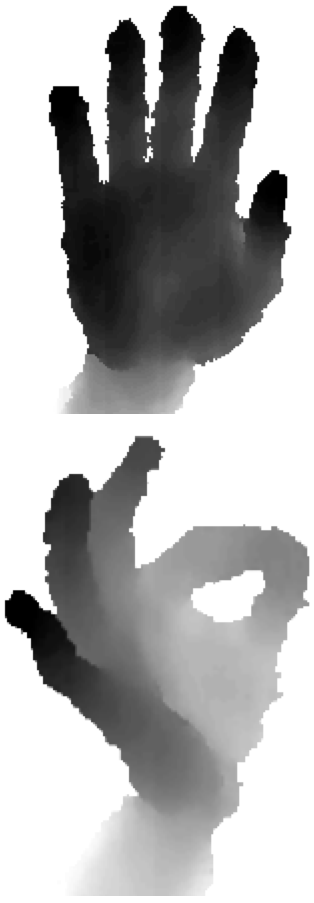
\includegraphics[width=0.75\textwidth]{figures_1_hand_tracking/Kinect_tiled}
                \caption{\footnotesize Sensor Depth}
        \end{subfigure}
        \begin{subfigure}{0.25\textwidth}
                \centering
                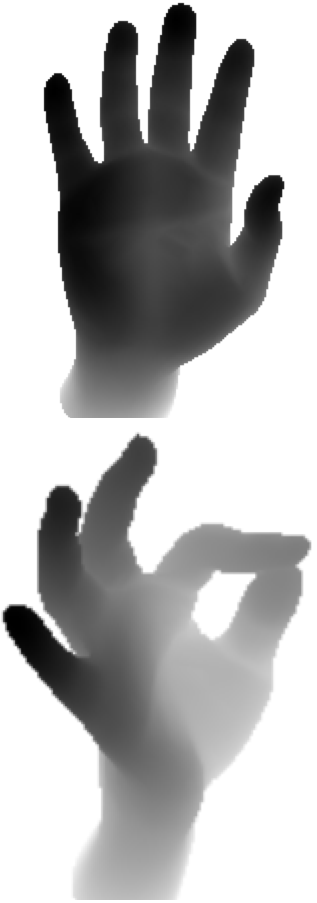
\includegraphics[width=0.75\textwidth]{figures_1_hand_tracking/Synthetic_tiled}
                \caption{\footnotesize Synthetic Depth}
        \end{subfigure}
        \begin{subfigure}{0.25\textwidth}
                \centering
                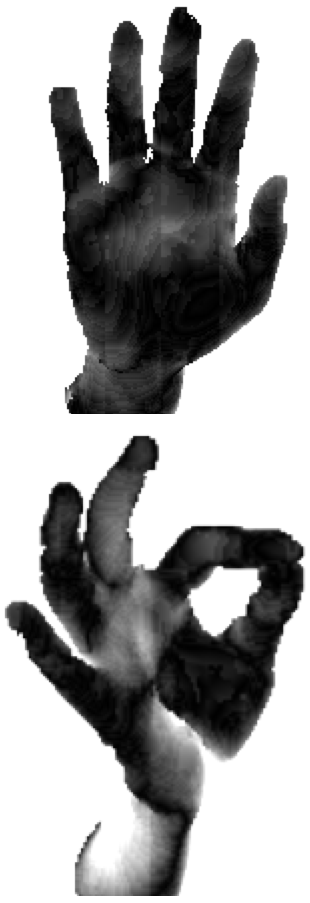
\includegraphics[width=0.75\textwidth]{figures_1_hand_tracking/Residue_tiled}
                \caption{\footnotesize Per-Pixel Error}
        \end{subfigure}
        \caption{Dataset Creation: Objective Function Data (with Libhand model~\protect\cite{libhand})}
        \label{fig:pso}
\end{figure}

Since we do not have a ground-truth measure for the 42 DOF hand model fitting, quantitative evaluation of this stage is difficult. \emph{Qualitatively}, the fitting accuracy was visually consistent with the underlying point cloud. An example of a fitted frame is shown in Figure \ref{fig:pso}. Only a very small number of poses failed to fit correctly; for these difficult poses, manual intervention was required.

One limitation of this system was that the frame rate of the PrimeSense camera (30fps) was not enough to ensure sufficient temporal coherence for correct convergence of the PSO optimizer. To overcome this, we had each user move their hands slowly during training data capture. Using a workstation with an Nvidia GTX 580 GPU and 4 core Intel processor, fitting each frame required 3 to 6 seconds. The final database consisted of 76,712 training set images, 2,421 validation set images and 2,000 test set images with their corresponding heat-maps, collected from multiple participants. A small sample of the test set images is shown in Figure \ref{fig:cnn_training_set_images}.

\begin{figure}[ht]
\centering
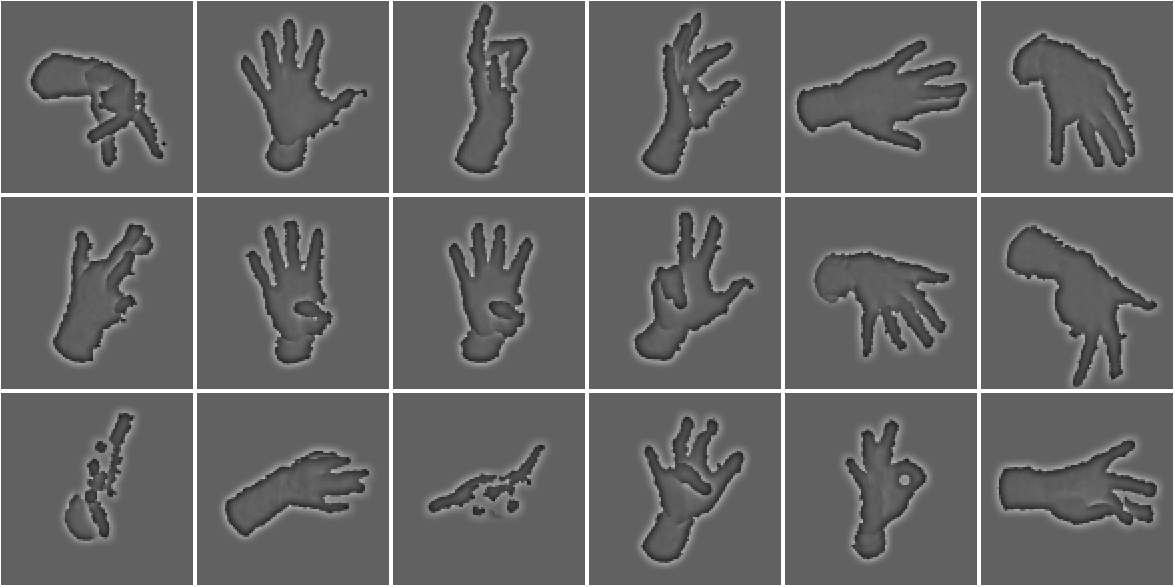
\includegraphics[width=0.8\columnwidth]{figures_1_hand_tracking/train_data_3_6}
    \caption{Sample ConvNet Test Set images}
    \label{fig:cnn_training_set_images}
\end{figure}

The ConvNet training took approximately 24 hours where early stopping is performed after 350 epochs to prevent overfitting. ConvNet hyper parameters, such as learning rate, momentum, L2 regularization, and architectural parameters (e.g., max-pooling window size or number of stages) were chosen by coarse meta-optimization to minimize a validation-set error. 2 stages of convolution (at each resolution level) and 2 fully-connected neural network stages were chosen as a tradeoff between numerous performance characteristics: generalization performance, evaluation time, and model complexity (or ability to infer complex poses). Figure \ref{fig:conv_learning_graph} shows the mean squared error (MSE) after each epoch. The MSE was calculated by taking the mean of sum-of-squared differences between the calculated 14 feature maps and the corresponding target feature maps.

\begin{figure}[ht]
\centering
\includegraphics[width=0.5\textwidth]{figures_1_hand_tracking/conv_learning_graph.pdf}
    \caption{ConvNet Learning Curve}
    \label{fig:conv_learning_graph}
\end{figure}

The mean UV error of the ConvNet heat-map output on the test set data was 0.41px (with standard deviation of 0.35px) on the 18x18 resolution heat-map image\footnote{To calculate this error we used the technique described in Section \ref{sec:realtimeposedetection} to calculate the heat-map UV feature location and then calculated the error distance between the target and ConvNet output locations}. After each heat-map feature was translated to the 640x480 depth image, the mean UV error was 5.8px (with standard deviation of 4.9px). Since the heat-map downsampling ratio is depth dependent, the UV error improves as the hand approaches the sensor. For applications that require greater accuracy, the heat-map resolution can be increased for better spatial accuracy at the cost of increased latency and reduced throughput.

\begin{table}[h]
\small
\centering
\begin{tabular}{lcc}
        \hline
        Feature Type           & Mean (px) & STD (px) \\
        \hline
        Palm                   & 0.33       & 0.30      \\
        Thumb Base \& Knuckle  & 0.33       & 0.43      \\
        Thumb Tip              & 0.39       & 0.55      \\
        Finger Knuckle         & 0.38       & 0.27      \\
        Finger Tip             & 0.54       & 0.33      \\
        \hline
    \end{tabular}
\caption{Heat-Map UV Error by Feature Type}
\label{tab:uv_errors}
\end{table}

Table~\ref{tab:uv_errors} shows the UV accuracy for each feature type. Unsurprisingly, we found that the ConvNet architecture had the most difficulty learning fingertip positions, where the mean error is 61\% higher than the accuracy of the palm features. The likely cause for this inaccuracy is twofold. Firstly, the fingertip positions undergo a large range of motion between various hand-poses and therefore the ConvNet must learn a more difficult mapping between local features and fingertip positions. Secondly, the PrimeSense Carmine 1.09 depth camera cannot always recover depth of small surfaces such as fingertips. The ConvNet is able to learn this noise behavior, and is actually able to approximate fingertip location in the presence of missing data, however the accuracy for these poses is low.

The computation time of the entire pipeline is 24.9ms, which is within our 30fps performance target. Within this period: decision forest evaluation takes 3.4ms, depth image preprocessing takes 4.7ms, ConvNet evaluation takes 5.6ms and pose estimation takes 11.2ms. The entire pipeline introduces approximately one frame of latency. For an example of the entire pipeline running in real-time as well as puppeteering of the LBS hand model, please refer to the supplementary video (screenshots from this video are shown in Figure~\ref{fig:screenshots}).

\begin{figure}[ht]
\centering
        \begin{subfigure}{0.3375\textwidth}
                \centering
                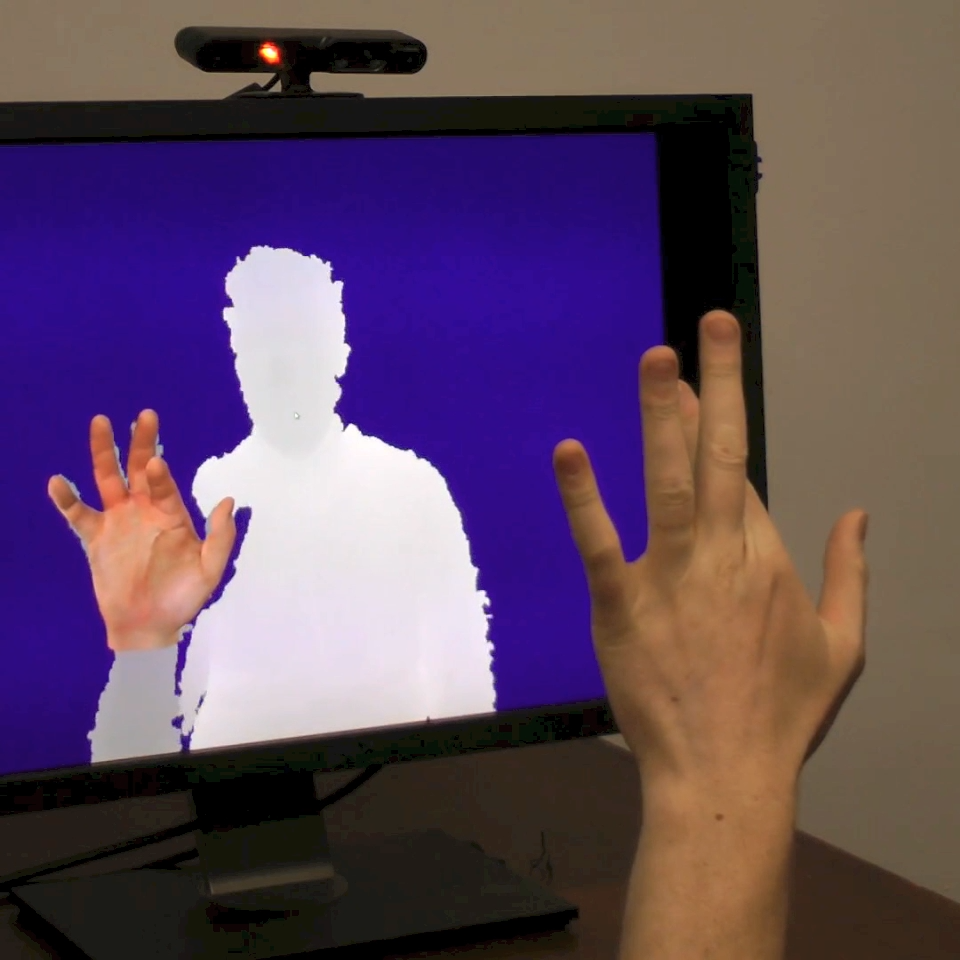
\includegraphics[width=\textwidth]{figures_1_hand_tracking/screenshot1_clipped}
                \caption{\footnotesize }
        \end{subfigure}
        \begin{subfigure}{0.28125\textwidth}
                \centering
                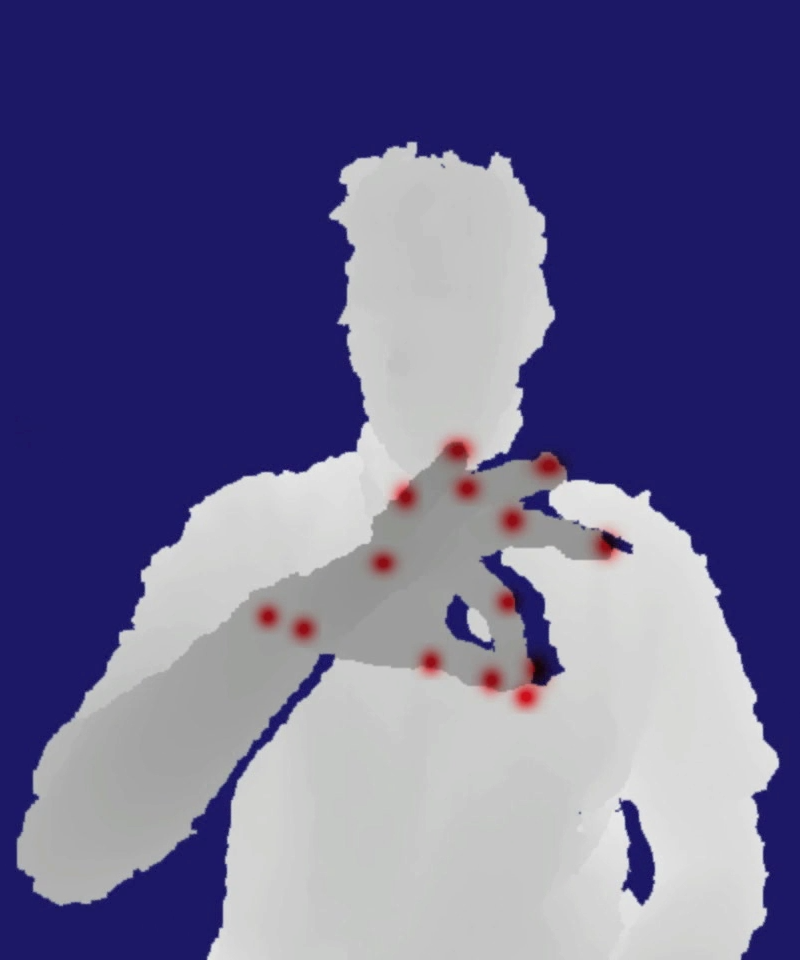
\includegraphics[width=\textwidth]{figures_1_hand_tracking/screenshot2_clipped}
                \caption{\footnotesize }
        \end{subfigure}
        \begin{subfigure}{0.28125\textwidth}
                \centering
                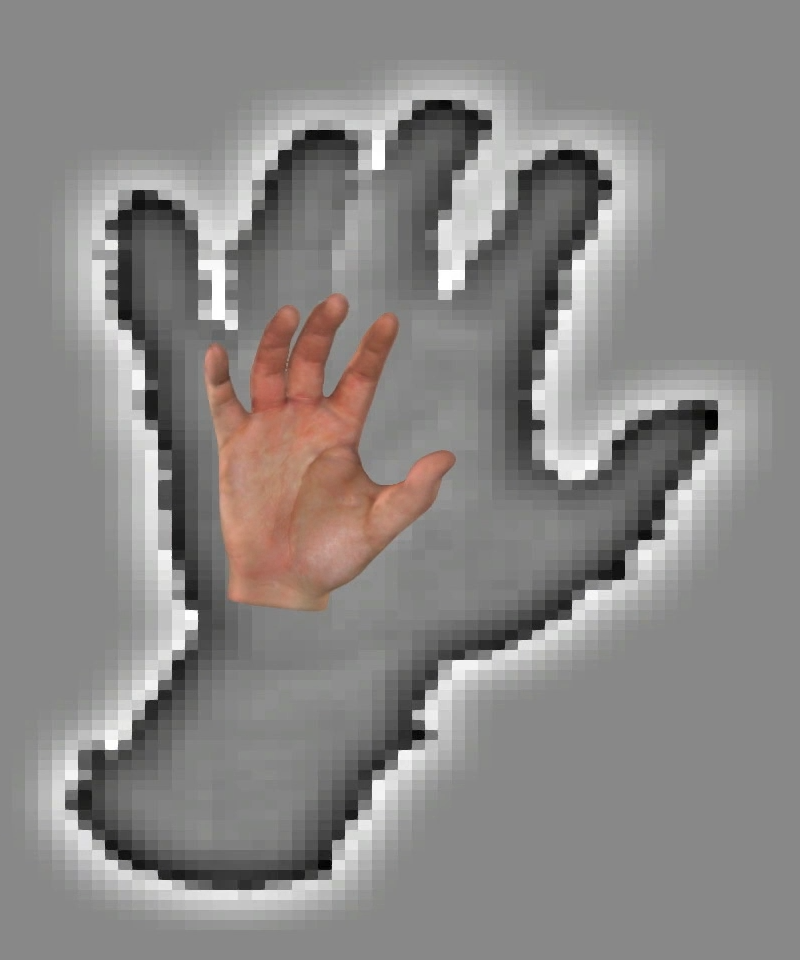
\includegraphics[width=\textwidth]{figures_1_hand_tracking/screenshot3_clipped}
                \caption{\footnotesize }
        \end{subfigure}
        \caption{Real-Time Tracking Results, a) Typical Hardware Setup, b) Depth with Heat-Map Features, c) ConvNet Input and Pose Output}
        \label{fig:screenshots}
\end{figure}

Figure~\ref{fig:fail_cases} shows three typical fail cases of our system. In \ref{fig:fail_cases}a) finite spatial precision of the ConvNet heat-map results in finger tip positions that are not quite touching. In \ref{fig:fail_cases}b) no similar pose exists in the database used to train the ConvNet, and for this example the network generalization performance was poor. In \ref{fig:fail_cases}c) the PrimeSense depth camera fails to detect the ring finger (the surface area of the finger tip presented to the camera is too small and the angle of incidence in the camera plane is too shallow), and the ConvNet has difficulty inferring the finger tip position without adequate support in the depth image, which results in an incorrect inferred position.

\begin{figure}[ht]
\centering
    \renewcommand{\tabcolsep}{0.02\linewidth}
    \begin{tabular}{ccc}
        \adjustbox{valign=m}{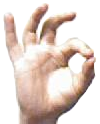
\includegraphics[width=0.2\linewidth]{figures_1_hand_tracking/fail_case0_rgb_clipped.png}} & \adjustbox{valign=m}{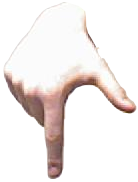
\includegraphics[width=0.2\linewidth]{figures_1_hand_tracking/fail_case1_rgb_clipped.png}} & \adjustbox{valign=m}{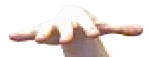
\includegraphics[width=0.2\linewidth]{figures_1_hand_tracking/fail_case2_rgb_clipped.png}} \\
        \adjustbox{valign=m}{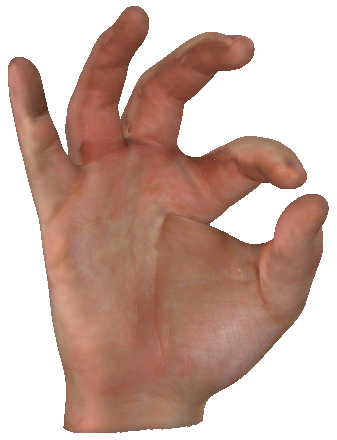
\includegraphics[width=0.2\linewidth]{figures_1_hand_tracking/fail_case0_model_clipped.png}} & \adjustbox{valign=m}{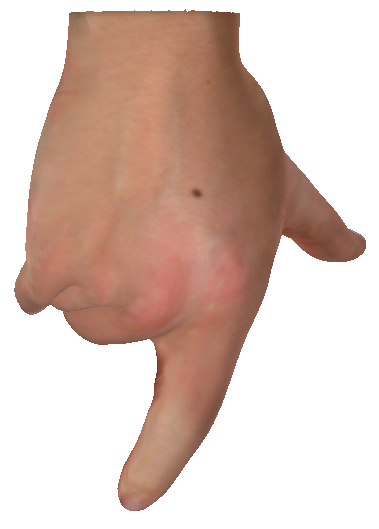
\includegraphics[width=0.2\linewidth]{figures_1_hand_tracking/fail_case1_model_clipped.png}} & \adjustbox{valign=m}{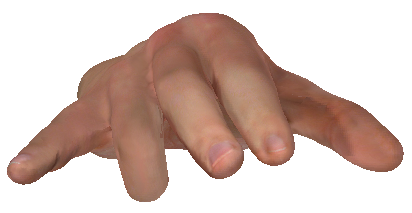
\includegraphics[width=0.2\linewidth]{figures_1_hand_tracking/fail_case2_model_clipped.png}} \\
        a) & b) & c)
    \end{tabular}
    \caption{Fail Cases: RGB ground-truth (top row), inferred model~\protect\cite{libhand} pose (bottom row)}
    \label{fig:fail_cases}
\end{figure}

Figure~\ref{fig:users} shows that the ConvNet output is tolerant for hand shapes and sizes that are not well represented in the ConvNet training set. The ConvNet and RDF training sets did not include any images for user b) and user c) (only user a)). We have only evaluated the system's performance on adult subjects. We found that adding a single per-user scale parameter to approximately adjust the size of the LBS model to a user's hand, helped the real-time IK stage better fit to the ConvNet output.

\begin{figure}[ht]
\centering
    \renewcommand{\tabcolsep}{0.006\linewidth}
    \begin{tabular}{ccc}
        % The SUM of all three image widths needs to be 0.31 * 3 \linewidth
        % User 1: 1136x1000 (rgb & depth) = 31.94% --> Width = 0.2970\linewidth
        % User 2: 1239x1000 (rgb & depth) = 34.83% --> Width = 0.3239\linewidth
        % User 3: 1182x1000 (rgb & depth) = 33.23% --> Width = 0.3090\linewidth
        % Total = 3557
        \adjustbox{valign=m}{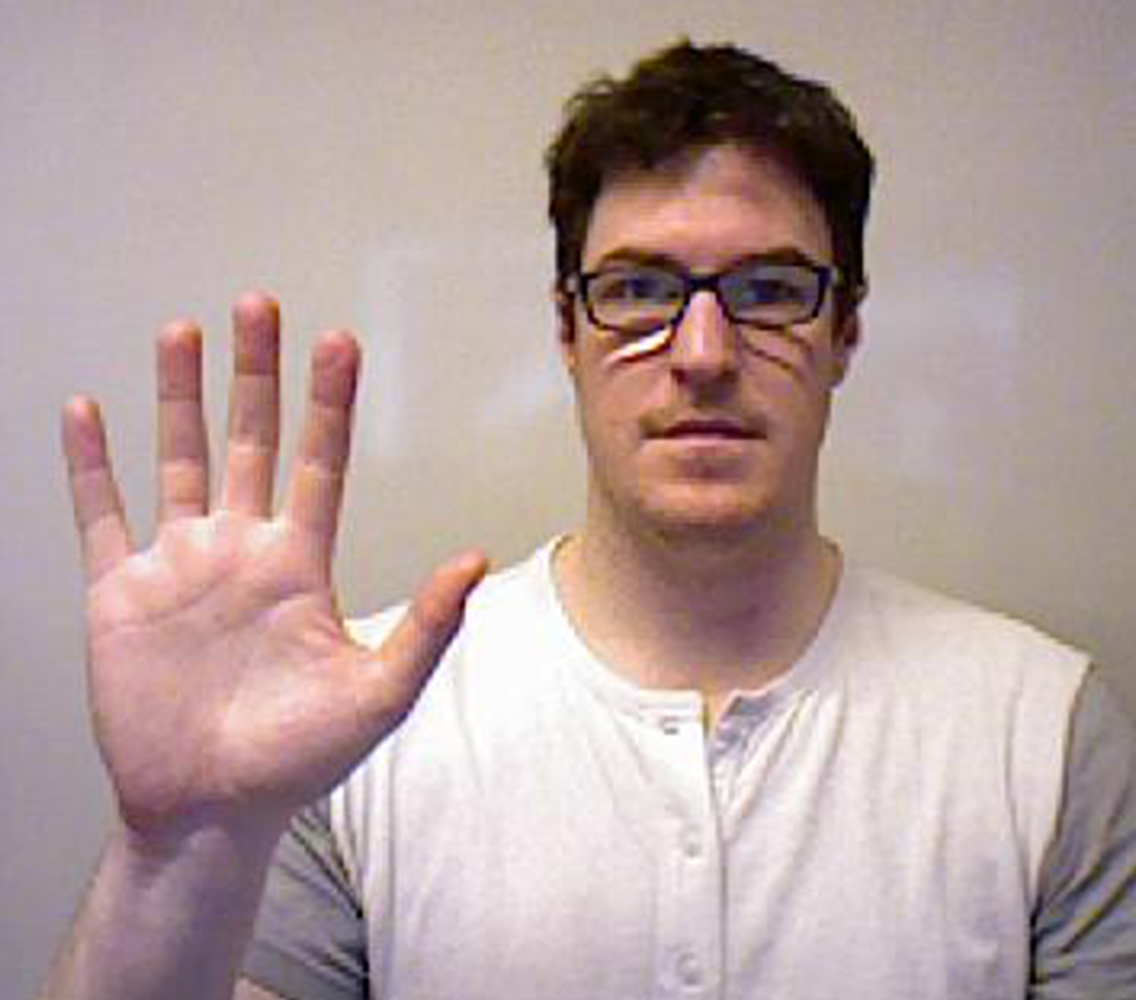
\includegraphics[width=0.2970\linewidth]{figures_1_hand_tracking/user1_rgb_cropped.png}} & \adjustbox{valign=m}{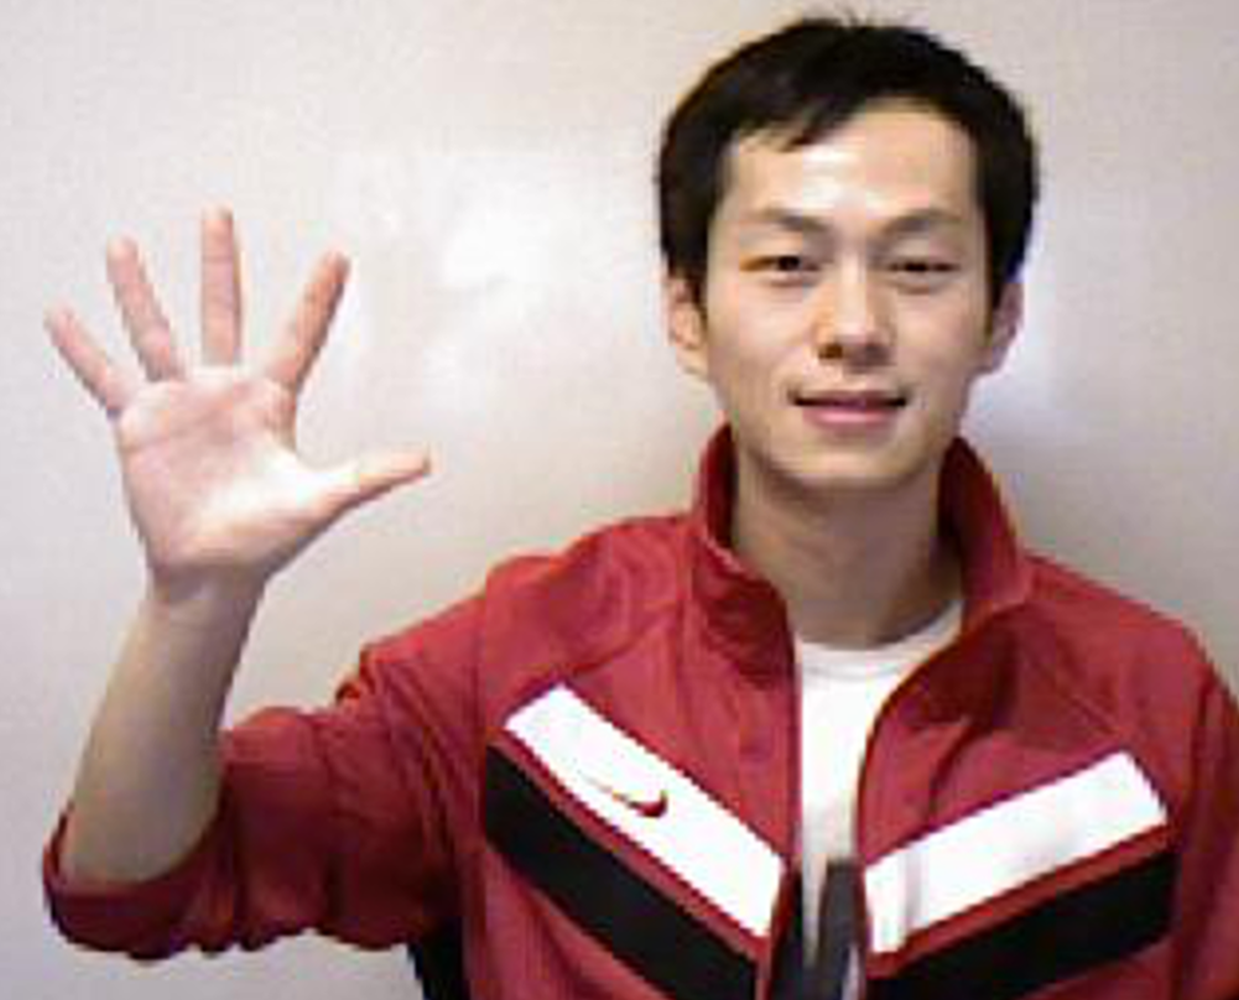
\includegraphics[width=0.3239\linewidth]{figures_1_hand_tracking/user2_rgb_cropped.png}} & \adjustbox{valign=m}{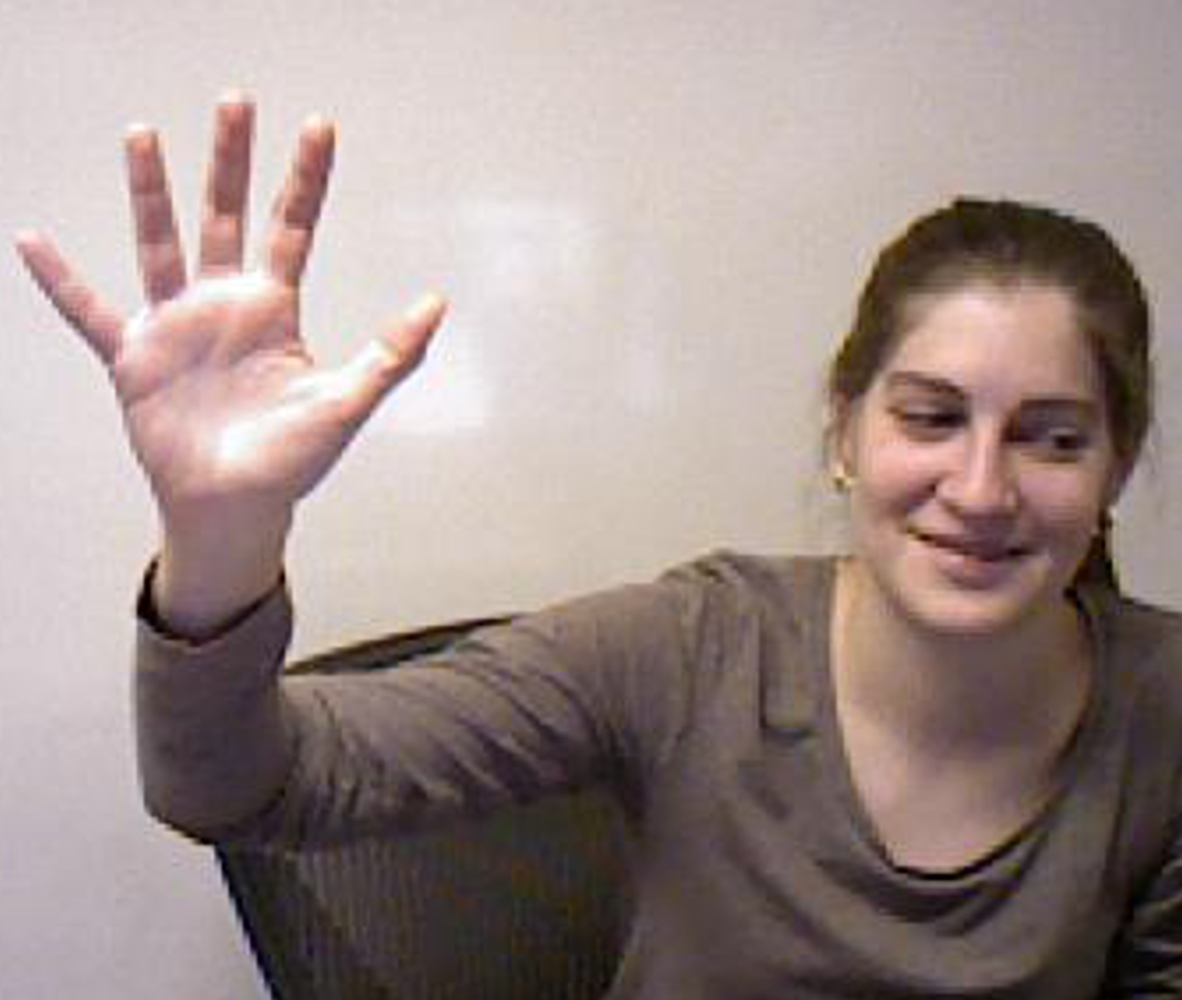
\includegraphics[width=0.3090\linewidth]{figures_1_hand_tracking/user3_rgb_cropped.png}} \\[0.98cm]
        \adjustbox{valign=m}{\includegraphics[width=0.2970\linewidth]{figures_1_hand_tracking/user1_depth_cropped_annotated.pdf}} & \adjustbox{valign=m}{\includegraphics[width=0.3239\linewidth]{figures_1_hand_tracking/user2_depth_cropped_annotated.pdf}} & \adjustbox{valign=m}{\includegraphics[width=0.3090\linewidth]{figures_1_hand_tracking/user3_depth_cropped_annotated.pdf}} \\[0.98cm]
        a) & b) & c)
    \end{tabular}
    \caption{Hand Shape/Size Tolerance: RGB ground-truth (top row), depth with annotated ConvNet output positions (bottom row)}
    \label{fig:users}
\end{figure}

Comparison of the relative real-time performance of this work with relevant prior art, such as that of \cite{3Gear} and \cite{Melax:2013}, is difficult for a number of reasons. Firstly, \cite{Melax:2013} uses a different capture device, which prevents fair comparison as it is impossible (without degrading sensor performance by using mirrors) for multiple devices to see the hand from the same viewpoint simultaneously. Secondly, no third-party ground truth database of poses with depth frames exists for human hands, so comparing the quantitative accuracy of numerous methods against a known baseline is not possible. More importantly however, is that the technique utilized by \cite{3Gear} is optimized for an entirely different use case and so fair comparison with their work is very difficult. \cite{3Gear} utilizes a vertically mounted camera, can track multiple hands simultaneously, and is computationally less expensive than the method presented in our work.

Figure~\ref{fig:compare} examines the performance of this work with the proprietary system of \cite{3Gear} (using the fixed-database version of the library), for 4 poses chosen to highlight the relative difference between the two techniques (images used with permission from 3Gear). We captured this data by streaming the output of both systems simultaneously (using the same RGBD camera). We mounted the camera vertically, as this is required for \cite{3Gear}, however our training set did not include any poses from this orientation.
Therefore, we expect our system to perform sub-optimally for this very different use case.

\begin{figure}[ht]
\centering
    \renewcommand{\tabcolsep}{0.006\linewidth}
    \resizebox{\linewidth}{!}{%
    \begin{tabular}{cccc}
        % The SUM of all four image widths needs to be (1 - 0.006 * 4) = 0.976 \linewidth
        % Pose A: 460x512 (rgb & depth) = 23.69% --> Width = 0.2312\linewidth
        % Pose B: 489x512 (rgb & depth) = 25.18% --> Width = 0.2457\linewidth
        % Pose C: 579x512 (rgb & depth) = 29.81% --> Width = 0.2910\linewidth
        % Pose D: 414x512 (rgb & depth) = 20.81% --> Width = 0.2081\linewidth
        % Total = 1942
        \adjustbox{valign=m}{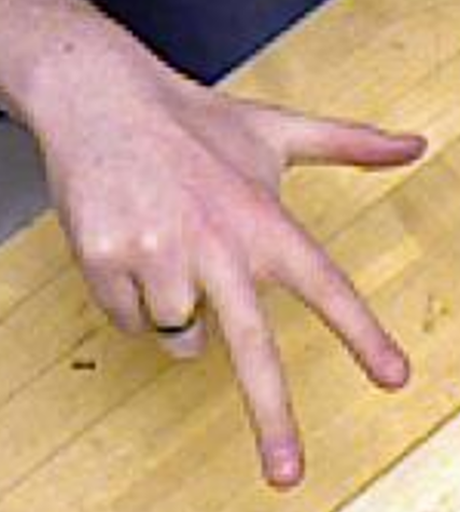
\includegraphics[width=0.2312\linewidth]{figures_1_hand_tracking/compare_a_rgb_cropped.png}} & \adjustbox{valign=m}{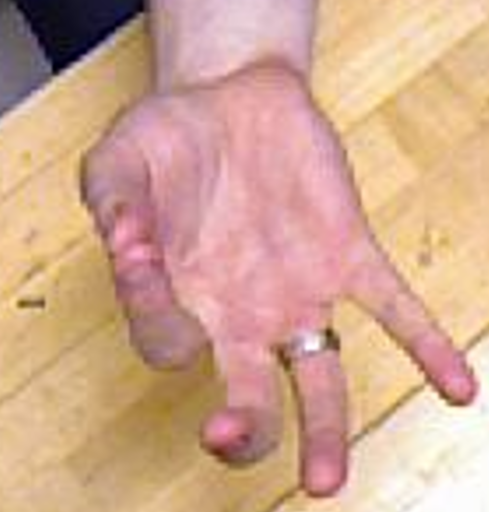
\includegraphics[width=0.2457\linewidth]{figures_1_hand_tracking/compare_b_rgb_cropped.png}} & \adjustbox{valign=m}{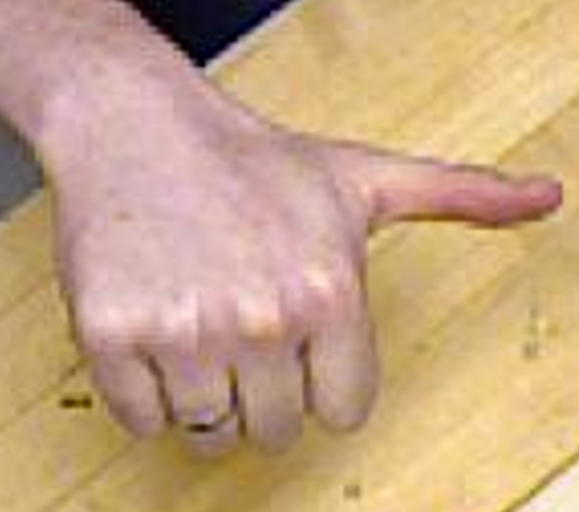
\includegraphics[width=0.2910\linewidth]{figures_1_hand_tracking/compare_c_rgb_cropped.png}} & \adjustbox{valign=m}{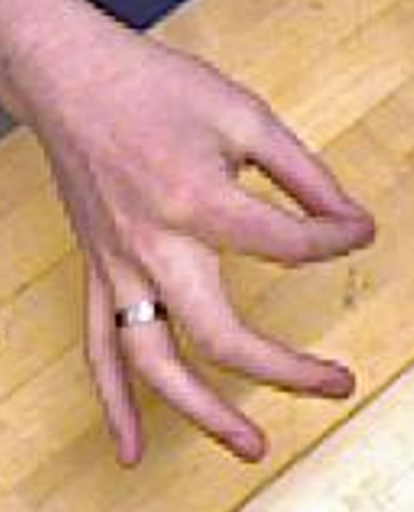
\includegraphics[width=0.2081\linewidth]{figures_1_hand_tracking/compare_d_rgb_cropped.png}} \\[0.98cm]
        \adjustbox{valign=m}{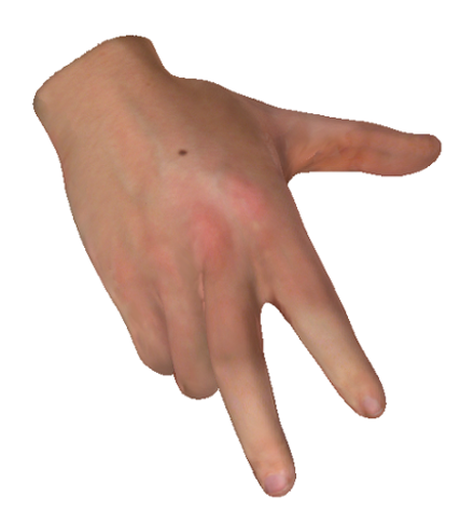
\includegraphics[width=0.2312\linewidth]{figures_1_hand_tracking/compare_a_ours_cropped.png}} & \adjustbox{valign=m}{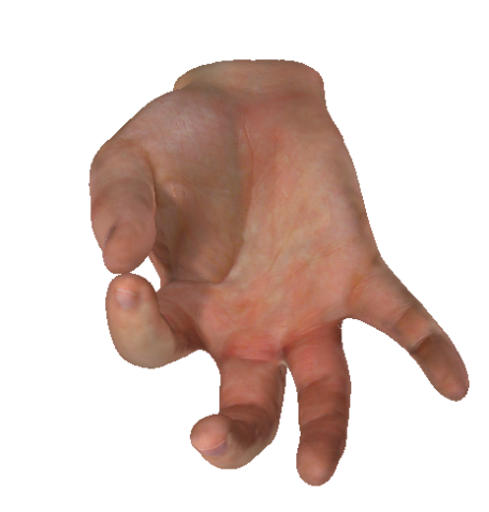
\includegraphics[width=0.2457\linewidth]{figures_1_hand_tracking/compare_b_ours_cropped.png}} & \adjustbox{valign=m}{\includegraphics[width=0.2910\linewidth]{figures_1_hand_tracking/compare_c_ours_cropped.png}} & \adjustbox{valign=m}{\includegraphics[width=0.2081\linewidth]{figures_1_hand_tracking/compare_d_ours_cropped.png}} \\[0.98cm]
        \adjustbox{valign=m}{\includegraphics[width=0.2312\linewidth]{figures_1_hand_tracking/compare_a_theirs_cropped.png}} & \adjustbox{valign=m}{\includegraphics[width=0.2457\linewidth]{figures_1_hand_tracking/compare_b_theirs_cropped.png}} & \adjustbox{valign=m}{\includegraphics[width=0.2910\linewidth]{figures_1_hand_tracking/compare_c_theirs_cropped.png}} & \adjustbox{valign=m}{\includegraphics[width=0.2081\linewidth]{figures_1_hand_tracking/compare_d_theirs_cropped.png}} \\[0.98cm]
        a) & b) & c) & d)
    \end{tabular}
    } % end resizebox
    \caption{Comparison with state-of-the-art commercial system: RGB ground-truth (top row), this work inferred model~\protect\cite{libhand} pose (middle row), \protect\cite{3Gear} inferred model pose (bottom row) (images used with permission from 3Gear).}
    \label{fig:compare}
\end{figure}

\section{Future Work}
\label{sec:future_work}

As indicated in Figure~\ref{fig:users}, qualitatively we have found that the ConvNet generalization performance to varying hand shapes is acceptable but could be improved. We are confident we can make improvements by adding more training data from users with different hand sizes to the training set.

For this work, only the ConvNet forward propagation stage was implemented on the GPU. We are currently working on implementing the entire pipeline on the GPU, which should improve performance of the other pipeline stages significantly. For example, the GPU ConvNet implementation requires 5.6ms, while the same network executed on the CPU (using optimized multi-threaded C++ code) requires 139ms.

The current implementation of our system can track two hands only if they are not interacting. While we have determined that the dataset generation system can fit multiple strongly interacting hand poses with sufficient accuracy, it is future work to evaluate the neural network recognition performance on these poses. Likewise, we hope to evaluate the recognition performance on hand poses involving interactions with non-hand objects (such as pens and other man-made devices).

While the pose recovery implementation presented in this work is fast, we hope to augment this stage by including a model-based fitting step that trades convergence radius for fit quality. Specifically, we suspect that replacing our final IK stage with an energy-based local optimization method, inspired by the work of Li et al.~\cite{li08global} could allow our method to recover second-order surface effects such as skin folding and skin-muscle coupling from very limited data, and still with low-latency. In addition to inference, such a localized energy-minimizing stage would enable improvements to the underlying model itself. Since these localized methods typically require good registration, our method, which gives correspondence from a single image could advance the state-of-the-art in non-rigid model capture.

Finally, we hope to augment our final IK stage with some form of temporal pose prior to reduce jitter; for instance, using an extended Kalman filter as a post-processing step to clean up the ConvNet feature output.

%
%\part{RGB-Based Localization of Human Bodies}
%\label{part:two}
%%\chapter{Overview\label{chap:2_body_tracking_overview}}

\section{Overview}

In Part~\ref{part:two} (with extensions in Parts~\ref{part:three} and \ref{part:four}) we will address the problem of inferring the 2D location of human joints in monocular RGB images - often called 2D body-pose detection. Recent approaches to this problem fall into two broad categories: 1) more traditional deformable part models \cite{modec} and 2) deep-learning based discriminative models \cite{deeppose, arjunaccv2014, jainiclr2014, tompson_efficient, tompsonnips2014}. Bottom-up part-based models are a common choice for this problem since the human body naturally segments into articulated parts. Traditionally these approaches have relied on the aggregation of hand-crafted low-level features such as SIFT~\cite{lowe1999object} or HoG~\cite{Dalal2005}, which are then input to a standard classifier or a higher level generative model. Care is taken to ensure that these engineered features are sensitive to the part that they are trying to detect and are invariant to numerous deformations in the input space (such as variations in lighting). On the other hand, discriminative deep-learning approaches learn an empirical set of low and high-level features which are typically more tolerant to variations in the training set and now outperform part-based models. However, incorporating priors about the structure of the human body (such as our prior knowledge about joint inter-connectivity) into such networks is difficult since the low-level mechanics of these networks is often hard to interpret. 

In this work we combine a ConvNet Part-Detector -- which alone outperformed all other existing methods at the time of publication~\cite{tompsonnips2014} -- with a part-based Spatial-Model into a unified learning framework. An overview of this architecture is shown in Figure~\ref{fig:overview_body_tracking}. In essence, this work is an attempt to combine the discriminative power of deep-learning with the inter-joint connectivity priors enforced by the more traditional deformable part models. In the first stage, we use a ConvNet to infer a probability distribution over spatial locations -- or heat-map -- describing the likelihood of each joint occurring in that spatial location (in Figure~\ref{fig:overview_body_tracking} there are 14 ground truth joints and so the ConvNet produces 14 heat-maps). The second stage graphical model inspired network then ``cleans up'' the noisy heat-map outputs to enforce correct inter-joint consistency.

\begin{figure}[th]
\centering
    \includegraphics[width=\columnwidth]{figures_2_body_tracking/overview}
    \caption{Network architecture overview}
  \label{fig:overview_body_tracking}
\end{figure}

Our translation-invariant ConvNet architecture utilizes a multi-resolution feature representation with overlapping receptive fields. Additionally, our Spatial-Model is able to approximate MRF loopy belief propagation, which is subsequently back-propagated through, and learned using the same learning framework as the Part-Detector. We show that the combination and joint training of these two models improves performance, and allows us to significantly outperform existing state-of-the-art models on the task of human body pose recognition.

\chapter{Architecture\label{chap:2_body_tracking_archiecture}}

\section{Model}

\subsection{Convolutional Network Part-Detector}
\label{sec:conv_model}
\begin{figure}[th]
\centering
    \includegraphics[width=\columnwidth]{figures_2_body_tracking/patch_model}
    \caption{Multi-Resolution Sliding-Window With Overlapping Receptive Fields}
  \label{fig:multiResPatchModel}
\end{figure}

The first stage of our detection pipeline is a deep ConvNet architecture for body part localization. The input is an RGB image containing one or more people and the output is a \emph{heat-map}, which produces a per-pixel likelihood for key joint locations on the human skeleton.

A \emph{sliding-window} ConvNet architecture is shown in Fig~\ref{fig:multiResPatchModel}. The network is slid over the input image to produce a dense heat-map output for each body-joint. Our model incorporates a \emph{multi-resolution} input with \emph{overlapping receptive fields}. The upper convolution bank in Fig~\ref{fig:multiResPatchModel} sees a standard 64x64 resolution input window, while the lower bank sees a larger 128x128 input context down-sampled to 64x64. The input images are then Local Contrast Normalized (LCN~\cite{torch7}) (after down-sampling with anti-aliasing in the lower resolution bank) to produce an approximate Laplacian pyramid. The advantage of using overlapping contexts is that it allows the network to see a larger portion of the input image with only a moderate increase in the number of weights. The role of the Laplacian Pyramid is to provide each bank with non-overlapping spectral content which minimizes network redundancy.

\begin{figure}[th]
  \centering
    \includegraphics[width=\columnwidth]{figures_2_body_tracking/oneshot_model}
    \caption{Efficient Sliding Window Model with Single Receptive Field}
  \label{fig:oneShotOneBank}
\end{figure}

An advantage of the Sliding-Window model (Fig~\ref{fig:multiResPatchModel}) is that the detector is translation invariant. However a major drawback is that evaluation is expensive due to redundant convolutions. Recent work~\cite{fastcnn,overfeatSermanet} has addressed this problem by performing the convolution stages on the full input image to efficiently create dense feature maps. These dense feature maps are then processed through convolution stages to replicate the fully-connected network at each pixel. An equivalent but efficient version of the sliding window model for a single resolution bank is shown in Fig~\ref{fig:oneShotOneBank}. Note that due to pooling in the convolution stages, the output heat-map will be a lower resolution than the input image.

For our Part-Detector, we combine an efficient sliding window-based architecture with multi-resolution and overlapping receptive fields; the subsequent model is shown in Fig~\ref{fig:oneShotMultiBank}. Since the large context (low resolution) convolution bank requires a stride of $\sfrac{1}{2}$ pixels in the lower resolution image to produce the same dense  output as the sliding window model, the bank must process four down-sampled images, each with a $\sfrac{1}{2}$ pixel offset, using shared weight convolutions. These four outputs, along with the high resolution convolution features, are processed through a 9x9 convolution stage (with 512 output features) using the same weights as the first fully connected stage (Fig~\ref{fig:multiResPatchModel}) and then the outputs of the low resolution bank are added and interleaved with the output of high resolution bank.

\begin{figure}[th]
  \centering
    \includegraphics[width=\columnwidth]{figures_2_body_tracking/one_shot_multires}
    \caption{Efficient Sliding Window Model with Overlapping Receptive Fields}
  \label{fig:oneShotMultiBank}
\end{figure}

While the above architecture gives optimal performance (and is exactly equivalent to the patch-based model), for our real-time system we simplify the above architecture by replacing the lower-resolution stage with a single convolution bank as shown in Fig~\ref{fig:oneShotMultiBankSimplified} and then upscale the resulting feature map. In all our practical implementation we use 3 resolution banks (but 2 banks are shown for brevity). Note that the simplified architecture is no longer equivalent to the original sliding-window network of Fig~\ref{fig:multiResPatchModel} since the lower resolution convolution features are effectively decimated and replicated leading into the fully-connected stage, however we have found empirically that the performance loss is minimal.

\begin{figure}[th]
  \centering
    \includegraphics[width=\columnwidth]{figures_2_body_tracking/one_shot_multires_ours}
    \caption{Approximation of Fig~\ref{fig:oneShotMultiBank}}
  \label{fig:oneShotMultiBankSimplified} 
\end{figure}

Supervised training of the network is performed using batched Stochastic Gradient Descent (SGD) with Nesterov Momentum. We use a Mean Squared Error (MSE) criterion to minimize the distance between the predicted output and a target heat-map. The target is a 2D Gaussian with a small variance and mean centered at the ground-truth joint locations. At training time we also perform random perturbations of the input images (randomly flipping and scaling the images) to increase generalization performance.

Note that an alternative model (such as in Tompson et al.~\cite{tompsonTOG14}) would replace the last 3 convolutional layers with a fully-connected neural network whose input context is the feature activations for the entire input image.  Such a model would be appropriate if we knew a priori that there existed a strong correlation between skeletal pose and the position of the person in the input frame since this alternative model is not invariant with respect to the translation of the person within the image.  However, the FLIC, LSP or MPII datasets have no such strong pose-location bias (i.e. a subject's torso is not always in the same location in the image), and therefore a sliding-window based architecture is more appropriate for our task.

\subsection{Higher-Level \emph{Spatial-Model}}
\label{sec:spatialmodel}

\begin{figure}[ht]
\centering
	\subcaptionbox{\footnotesize False Positive\label{fig:conv_net_fail_a}}{\includegraphics[height=5.5cm]{figures_2_body_tracking/part_detector_fail1}}
	\subcaptionbox{\footnotesize Multiple Subjects\label{fig:conv_net_fail_b}}{\includegraphics[height=5.5cm]{figures_2_body_tracking/part_detector_fail2}}
        \caption{ConvNet Part Detector Fail Cases}
        \label{fig:conv_net_fail}
\end{figure}

The Part-Detector (Section~\ref{sec:conv_model}) performance on our validation set predicts heat-maps that contain many false positives and poses that are anatomically incorrect; for instance when a peak for face detection is unusually far from a peak in the corresponding shoulder heat-map. Figures~\ref{fig:conv_net_fail_a} and \ref{fig:conv_net_fail_b} show two additional fail cases; 1) when a strong false positive outlier results in an incorrectly predicted joint location and 2) when strong activations from another subject in the frame result in an incorrectly labeled joint. Even in the presence of foreshortening, in both these cases it is clear that given the length of the correctly labeled limbs, one should be able to improve the prediction given that the incorrectly labeled limbs are anatomically incorrect.

In spite of the improved Part-Detector context (using our technique of overlapping receptive fields), the feed forward network still has difficulty learning an implicit model of the constraints of the body parts for the full range of body poses. We use a higher-level \emph{Spatial-Model} to constrain joint inter-connectivity and enforce global pose consistency. The expectation of this stage is to not increase the performance of detections that are already close to the ground-truth pose, but to remove false positive outliers that are anatomically incorrect.

\begin{figure}[th]
  \centering
    \includegraphics[width=0.6\columnwidth]{figures_2_body_tracking/mrf1}
    \caption{Linear chain MRF}
  \label{fig:mrf1} 
\end{figure}

Similar to Jain et al.~\cite{jainiclr2014}, we formulate the \emph{Spatial-Model} as an MRF model over the distribution of spatial locations for each body part.  The spatial model of \cite{jainiclr2014} is shown in Figure~\ref{fig:mrf1}. $\tilde{f}$, $\tilde{s}$, $\tilde{e}$, $\tilde{w}$, $f$, $s$, $e$, and $w$ are 2D random variables (or random Matrices), describing the likelihood of the face, shoulder, elbow and wrist joints for each pixel location in the input image \footnote{note that due to downsampling in the part detector this will be at a lower resolution than the input, and we use nearest-neighbor up-sampling to bring the heat-maps into the original resolution}. $\tilde{f}$, $\tilde{s}$, $\tilde{e}$ and $\tilde{w}$ are the noisy heat-maps from the ConvNet output (Section~\ref{sec:conv_model}) (or visible variables) and $f$, $s$, $e$, and $w$ are the clean heat-maps (or hidden variables) that we are trying to infer. Note that in practice, the full tree for the LSP dataset will include 14 nodes and the tree for the FLIC dataset will include 7 nodes, one node for each of the joints we are trying to infer.  For brevity only 4 nodes are shown.

$\phi(f)$, $\phi(s)$, $\phi(e)$ and $\phi(w)$ are the unary potentials (or sometimes called an image evidence function when the factor between the hidden and visible variables is a 2D tensor), and $\psi(f,s)$, $\psi(s,e)$ and $\psi(e,w)$ are the pair-wise factors describing the joint priors between adjacent neighbors in the linear chain-MRF. As we will see, these priors enforce inter-joint consistency.  Using these factors, we can describe the joint probability distribution as a product of factors, normalized by the partition function $Z$:

\begin{equation}
\bar{p}\left(f,s,e,w,\tilde{f},\tilde{s},\tilde{e},\tilde{w}\right) = \frac{1}{Z}\prod_{i,j}\psi\left(x_i,x_j\right)\prod_{k}\phi\left(x_k\right)
\label{eq:mrf1}
\end{equation}

The goal of our network is then to infer the distributions of the hidden variables $f$, $s$, $e$ and $w$ by marginalization of other variables in the joint distribution. One such method is to use a belief propagation formulation, which can be shown to converge to an exact solution given that the MRF in Figure~\ref{fig:mrf1} is a tree-structured graph. After a single round of belief propagation, the belief of a variable $x_i$ is given by the product of incoming messages from each neighbor joint $j$, $m_{ji}\left(x_i\right)$, multiplied by the unary factor for the joint $\psi\left(x_i\right)$: 

\begin{equation}
b\left(x_i\right)=k\phi\left(x_i\right)\prod_{j\in N(i)}m_{ji}\left(x_i\right) \\
\label{eq:mrf1_message_passing}
\end{equation}

Here $k$ is a normalizing partition function. Each incoming message from joint $j$ to joint $i$ is described by the product of incoming messages to joint $j$ from it's neighbors not including $i$ (i.e. in the set $N(j)-\{i\}$, where $N(j)$ is the set of adjacent neighbors for node $j$), multiplied with the marginalized product of the unary potential for node $j$, $\psi\left(x_j\right)$, and the pair-wise factor between $i$ and $j$, $\psi\left(x_j, x_i\right)$:

\begin{equation}
m_{ji}\left(x_i\right) \leftarrow \sum_{x_j}\phi\left(x_j\right)\psi\left(x_j,x_i\right)\prod_{k\in N(j) - \{i\}}m_{kj}\left(x_j\right)
\end{equation}

Since the height of our tree is 3, it can also be shown that message passing will converge to the exact solution after 3 rounds. Writing out the full expression for the marginalization of the hidden variable for the face joint we get:

\begin{equation}
b\left(f\right)=k\phi(f)\sum_s \phi(s)\psi(s,f)\sum_e \phi(e)\psi(e,s) \sum_w \phi(w)\psi(w,e)
\label{eq:face_marginal}
\end{equation}

Note that we can also arrive at the same solution by marginalizing the joint distribution of Equation~\ref{eq:mrf1}, however the belief propagation formulation provides us with invaluable insight as to the function of the pair-wise prior as we will show. Note that the expression in Equation~\ref{eq:face_marginal}, requires sequential calculation of a 4D tensor and 2D tensor products (for the multiplication of the pairwise and unary potentials), which is then integrated over 2D to calculate the marginalized message distribution. To re-phrase the above formation so that it is more amenable to implementation as a neural network, we simplify Equation~\ref{eq:face_marginal}:

\begin{equation}
b\left(f\right)\approx k\phi(f)\prod_i\sum_{x_i} \phi(x_i)\psi(x_i,f)
\label{eq:face_marginal_simple}
\end{equation}

This means that rather than sequentially taking each product and multiplying before marginalizing, the messages from adjacent joints can be calculated in parallel, which as we shall see, is easier to implement as a single layer of neural network. However, by doing so we have actually changed the structure of the MRF; the new formulation is a star graph as shown in Figure~\ref{fig:mrf2} (visible nodes are not shown for brevity).

\begin{figure}[th]
  \centering
    \includegraphics[width=\columnwidth]{figures_2_body_tracking/mrf2}
    \caption{Star MRF}
  \label{fig:mrf2} 
\end{figure}

Note that Equation~\ref{eq:face_marginal_simple} is effectively a separate star graph for each of the joint marginals that we will calculate, i.e. the marginalized hidden variable we infer for the face joint, is not the same as the variable we use for the shoulder joint.  Also not that we have weakened our pair-wise priors; instead of modeling the tight coupling between the shoulder and wrist, when incorporating evidence for marginalization of the face, instead we will model the much looser pair-wise distribution of the wrist to face joint. Since the average displacement between the face and wrist joint is large, the prior distribution will not have high entropy and will therefore have a smaller impact on the marginalized face distribution.

The 4D $\times$ 2D tensor product of the pairwise and unary factors as written in Equation~\ref{eq:face_marginal_simple} is extremely expensive to calculate. We therefore make one important approximation, instead of performing the tensor product then marginalizing, we instead replace this with a convolution operator and use a `conditional pairwise' factor as shown in Equation~\ref{eq:conv_prior}. By doing so our implicit assumption is that the distribution of a joint`s location given the location of another joint is independent of the position in the input image, i.e., the expected displacement between joints is the same and is independent of the limb`s position in the image. In our model this is a fair assumption for 2 reasons: 1) we expect that the movement of a joint is independent of the person`s location in an image and 2) we want to formulate a detector architecture that is translation invariant and so modeling the full factor as a convolutional prior will achieve this.

\begin{equation}
b^\prime\left(f\right)\approx k\phi(f)\prod_i \phi(x_i)\ast\psi(x_i|f)
\label{eq:conv_prior}
\end{equation}

Note that this new formulation is no longer a traditional MRF, however it is still a graphical model that is able to capture the inter-dependancies between joints.  Lastly, we add a scalar bias term, $b_{x_i|j}$, to each of the messages:

\begin{equation}
b^\prime\left(f\right)\approx k\phi(f)\prod_i \phi(x_i)\ast\psi(x_i|f) + b_{x_i|f}
\label{eq:final_equation}
\end{equation}

This bias essentially sets a background probability distribution. This bias is extremely important since the ConvNet may output false negatives, particularly for difficult joints like the wrist and ankle, which results in a product with a zero probability, causing strong positive activations for neighbor joints to be incorrectly attenuated. The ratio between the dynamic range of the conditional prior and the strength of the bias term sets how much a neighbor joint ``trusts" the incoming message, and for strongly coupled joints (like the face and shoulder), we indeed find that the network learns to set the background bias close to zero during training. In contrast, for loosely coupled joints (such as wrist and face), the network will learn to set the bias high and the dynamic range of the prior term small.

Fig~\ref{fig:heat_map_examples} shows a practical example of how the Spatial-Model is able to remove an anatomically incorrect strong outlier from the face heat-map by incorporating the presence of a strong shoulder detection. For simplicity, only the shoulder and face joints are shown, however, this example can be extended to incorporate all body part pairs. If the shoulder heat-map shown in Fig~\ref{fig:heat_map_examples} had an incorrect false-negative (i.e. no detection at the correct shoulder location), the addition of the background bias $b_{v\rightarrow A}$ would prevent the output heat-map from having no maxima in the detected face region.

\begin{figure}[th]
  \centering
    \includegraphics[width=\columnwidth]{figures_2_body_tracking/spatial}
    \caption{Didactic Example of Message Passing Between the Face and Shoulder Joints}
  \label{fig:heat_map_examples}
\end{figure}

Fig~\ref{fig:heat_map_examples} contains the conditional distributions for face and shoulder parts learned on the FLIC~\cite{modec} dataset. For any part $x_i$ the distribution $\psi\left(x_i,x_j\right)$ is the identity map, and so the message passed from any joint to itself is its unary distribution. Since the FLIC dataset is biased towards front-facing poses where the right shoulder is directly to the lower right of the face, the model learns the correct spatial distribution between these body parts and has high probability in the spatial locations describing the likely displacement between the shoulder and face. For datasets that cover a larger range of the possible poses (for instance the LSP~\cite{Johnson10} dataset), we would expect these distributions to be less tightly constrained, and therefore this simple Spatial-Model will be less effective. 

For our practical implementation we treat the distributions above as energies to avoid the evaluation of $k$ in Equation~\ref{eq:final_equation}. There are 3 reasons why we do not include the partition function. Firstly, we are only concerned with the maximum output value of our network, and so we only need the output energy to be proportional to the normalized distribution. Secondly, since both the part detector and spatial model parameters contain only shared weight (convolutional) parameters that are equal across pixel positions, evaluation of the partition function during back-propagation will only add a scalar constant to the gradient weight, which would be equivalent to applying a per-batch learning-rate modifier. Lastly, since the number of parts is not known a priori (since there can be unlabeled people in the image), and since the distributions $p_v$ describe the part location of a single person, we cannot normalize the Part-Model output. Our final model is a modification to Eq~\ref{eq:final_equation}:

\begin{align}
\label{eq:mrf2}
\bar{e}_A = \operatorname{exp}\left(\sum_{v\in V}\left[\operatorname{log}\left(\operatorname{SoftPlus}\left(e_{A|v}\right) \ast \operatorname{ReLU}\left(e_v\right) + \operatorname{SoftPlus}\left(b_{v\rightarrow A}\right)\right)\right]\right) \\
\text{where: } \operatorname{SoftPlus}\left(x\right) = \sfrac{1}{\beta} \operatorname{log}\left(1+\operatorname{exp}\left(\beta x\right)\right)\text{, } \sfrac{1}{2} \leq\beta\leq 2 \notag \\
\operatorname{ReLU}\left(x\right) = \operatorname{max}\left(x, \epsilon \right)\text{, } 0<\epsilon\leq 0.01\notag
\end{align}

The network-based implementation of Eq~\ref{eq:mrf2} is shown in Fig~\ref{fig:spatial_model_network}. Eq~\ref{eq:mrf2} replaces the outer multiplication of Eq~\ref{eq:final_equation} with a log space addition to improve numerical stability and to prevent coupling of the convolution output gradients (the addition in log space means that the partial derivative of the loss function with respect to the convolution output is not dependent on the output of any other stages). However, this then requires that our output criterion be before the outer exp, however for visualization the exp is required. The inclusion of the \emph{SoftPlus} and \emph{ReLU} stages on the weights, biases and input heat-map maintains a strictly greater than zero convolution output, which prevents numerical issues for the values leading into the \emph{Log} stage. Finally, a \emph{SoftPlus} stage is used to maintain continuous and non-zero weight and bias gradients during training. With this modified formulation, Eq~\ref{eq:mrf2} is trained using back-propagation and SGD.

\begin{figure}[th]
  \centering
    \includegraphics[width=\columnwidth]{figures_2_body_tracking/spatial_model}
    \caption{Single Round Message Passing Network}
  \label{fig:spatial_model_network}
\end{figure}

The convolution sizes are adjusted so that the largest joint displacement is covered within the convolution window. For our 90x60 pixel heat-map output, this results in large 128x128 convolution kernels to account for a joint displacement radius of 64 pixels (note that padding is added on the heat-map input to prevent pixel loss). Therefore for such large kernels we use FFT convolutions based on the GPU implementation by Mathieu et al.~\cite{fft}.

The convolution weights are initialized using the empirical histogram of joint displacements created from the training examples. This initialization improves learned performance, decreases training time and improves optimization stability. During training we randomly flip and scale the heat-map inputs to improve generalization performance.

The FLIC and LSP datasets contain many frames with more than a single person, while the joint locations from only one person in the scene are labeled. Therefore an approximate torso bounding box is provided at test time for the single labeled person in the scene. We incorporate this data by including an extra ``torso-joint heat-map" to the input of the Spatial-Model so that it can learn to select the correct feature activations in a cluttered scene as shown in Figure~\ref{fig:torso_input}.

\begin{figure}[th]
  \centering
    \includegraphics[width=0.8\columnwidth]{figures_2_body_tracking/torso_input}
    \caption{Torso heat-map utilization}
  \label{fig:torso_input}
\end{figure}

\subsection{Unified Model}
\label{sec:unified}

Since our Spatial-Model (Section~\ref{sec:spatialmodel}) is trained using back-propagation, we can combine our Part-Detector and Spatial-Model stages in a single \emph{Unified Model}. To do so, we first train the Part-Detector separately and store the heat-map outputs. We then use these heat-maps to train a Spatial-Model. Finally, we combine the trained Part-Detector and Spatial-Models and back-propagate through the entire network.

This unified fine-tuning further improves performance. We hypothesize that because the Spatial-Model is able to effectively reduce the output dimension of possible heat-map activations, the Part-Detector can use available learning capacity to better localize the precise target activation.

\chapter{Experimental Results\label{chap:2_body_tracking_experimental}}

\section{Results}

The models from Sections \ref{sec:conv_model} and \ref{sec:spatialmodel} were implemented within the Torch7~\cite{torch7} framework (with custom GPU implementations for the non-standard stages above). Training the Part-Detector takes approximately 48 hours, the Spatial-Model 12 hours, and forward-propagation for a single image through both networks takes 51ms \footnote{We use a 12 CPU workstation with an NVIDIA Titan GPU}.

\begin{figure}[th]
  \centering
    \includegraphics[width=\columnwidth]{figures_2_body_tracking/flic_plus_sample}
    \caption{Sample images from FLIC-plus dataset}
  \label{fig:flic_plus}
\end{figure}

We evaluated our architecture on the FLIC~\cite{modec} and extended-LSP~\cite{Johnson10} datasets. These datasets consist of still RGB images with 2D ground-truth joint information generated using Amazon Mechanical Turk. The FLIC dataset is comprised of 5003 images from Hollywood movies with actors in predominantly front-facing standing up poses (with 1016 images used for testing), while the extended-LSP dataset contains a wider variety of poses of athletes playing sport (10442 training and 1000 test images).

The FLIC-full dataset contains 20928 training images, however many of these training set images contain samples from the 1016 test set scenes and so would allow unfair over-training on the FLIC test set. Therefore, we propose a new dataset - called \emph{FLIC-plus} (\href{http://cims.nyu.edu/~tompson/flic_plus.htm}{http://cims.nyu.edu/$\sim$tompson/flic\_plus.htm}) - which is a 17380 image subset from the FLIC-plus dataset. Sample images from this dataset are shown in Figure~\ref{fig:flic_plus}. To create this dataset, we produced unique scene labels for both the FLIC test set and FLIC-plus training sets using Amazon Mechanical Turk. We then removed all images from the FLIC-plus training set that shared a scene with the test set. Since 253 of the sample images from the original 3987 FLIC training set came from the same scene as a test set sample (and were therefore removed by the above procedure), we added these images back so that the FLIC-plus training set is a superset of the original FLIC training set. Using this procedure we can guarantee that the additional samples in FLIC-plus are sufficiently independent to the FLIC test set samples.

For evaluation of the test-set performance we use the measure suggested by Sapp et. al.~\cite{modec}. For a given normalized pixel radius (normalized by the torso height of each sample) we count the number of images in the test-set for which the distance of the predicted UV joint location to the ground-truth location falls within the given radius.

Fig~\ref{fig:flic_elbow} and \ref{fig:flic_wrist} show our model's performance on the the FLIC test-set for the elbow and wrist joints respectively and trained using both the FLIC and FLIC-plus training sets. Performance on the LSP dataset is shown in Fig~\ref{fig:lsp_best} and \ref{fig:lsp_best_lower}. For LSP evaluation we use person-centric (or non-observer-centric) coordinates for fair comparison with prior work~\cite{deeppose,dantone13cvpr}. Our model outperforms existing state-of-the-art techniques on both of these challenging datasets with a considerable margin.

\begin{figure}[th]
  \centering
  \begin{subfigure}[b]{0.63\textwidth}
    \begin{subfigure}[b]{0.99\textwidth}
         % Trim is left, bottom, right, top
          \begin{flushright}
                  \includegraphics[trim=0cm 0.6cm 1.1cm 0.6cm, clip=true, width=0.95\textwidth]{figures_2_body_tracking/flic_legend.pdf}
          \end{flushright}
      \end{subfigure}
    \hfill

    \begin{subfigure}[b]{0.49\textwidth}
          \includegraphics[width=\textwidth]{figures_2_body_tracking/best_flic_elbow.pdf}
          \caption{FLIC: Elbow}
          \label{fig:flic_elbow}
    \end{subfigure}
    \begin{subfigure}[b]{0.49\textwidth}
          \includegraphics[width=\textwidth]{figures_2_body_tracking/best_flic_wrist.pdf}
          \caption{FLIC: Wrist}
          \label{fig:flic_wrist}
    \end{subfigure}
  \end{subfigure}
  \begin{subfigure}[b]{0.307\textwidth}
        \includegraphics[width=\textwidth]{figures_2_body_tracking/best_lsp.pdf}
        \caption{LSP: Wrist and Elbow}
        \label{fig:lsp_best}
  \end{subfigure}
  \caption{Model Performance}
  \label{fig:flic_results}
\end{figure} 

Fig~\ref{fig:spatial_model_performance} illustrates the performance improvement from our simple Spatial-Model. As expected the Spatial-Model has little impact on accuracy for low radii threshold, however, for large radii it increases performance by 8 to 12\%. Unified training of both models (after independent pre-training) adds an additional 4-5\% detection rate for large radii thresholds. 

\begin{figure}[th]
  \centering
  \begin{subfigure}[b]{0.31\textwidth}
        \includegraphics[width=\textwidth]{figures_2_body_tracking/best_lsp_lower.pdf}
        \caption{LSP: Ankle and Knee}
        \label{fig:lsp_best_lower}
  \end{subfigure}
  \begin{subfigure}[b]{0.31\textwidth}
        \includegraphics[width=\textwidth]{figures_2_body_tracking/spatial_model_performance.pdf}
        \caption{FLIC: Wrist}
        \label{fig:spatial_model_performance}
  \end{subfigure}
  \begin{subfigure}[b]{0.31\textwidth}
        \includegraphics[width=\textwidth]{figures_2_body_tracking/banks.pdf}
        \caption{FLIC: Wrist}
        \label{fig:banks}
  \end{subfigure} 
  \caption{(a) Model Performance (b) With and Without Spatial-Model (c) Part-Detector Performance Vs Number of Resolution Banks (FLIC subset)}
  \label{fig:lsp_results_1}
\end{figure}

The impact of the number of resolution banks is shown in Fig~\ref{fig:banks}). As expected, we see a big improvement when multiple resolution banks are added. Also note that the size of the receptive fields as well as the number and size of the pooling stages in the network also have a large impact on the performance. We tune the network hyper-parameters using coarse meta-optimization to obtain maximal validation set performance within our computational budget (less than 100ms per forward-propagation).

Fig~\ref{fig:pics} shows the predicted joint locations for a variety of inputs in the FLIC and LSP test-sets. Our network produces convincing results on the FLIC dataset (with low joint position error), however, because our simple Spatial-Model is less effective for a number of the highly articulated poses in the LSP dataset, our detector results in incorrect joint predictions for some images. We believe that increasing the size of the training set will improve performance for these difficult cases.
% Source images are 720x480 or 1.5:1 aspect ratio --> We want the output aspect ratio to be 0.7058:1

\begin{figure}[th]
  \centering
  \adjustbox{trim={0.2\width} {0.075\height} {0.475\width} {.2\height},clip,height=0.256\textwidth}% Trim is left bottom right top
      {\includegraphics[width=\textwidth]{figures_2_body_tracking/pred_along-came-polly-00117171_02592.pdf}}
  \adjustbox{trim={0.0\width} {0.15\height} {0.6\width} {.1\height},clip,height=0.256\textwidth}
      {\includegraphics[width=\textwidth]{figures_2_body_tracking/pred_bend-of-the-river-00116721_06712.pdf}}
  \adjustbox{trim={0.2\width} {0.15\height} {0.5\width} {.2\height},clip,height=0.256\textwidth}
      {\includegraphics[width=\textwidth]{figures_2_body_tracking/pred_funny-girl-dvd-video-00184781_09440.pdf}}
  \adjustbox{trim={0.01\width} {0.15\height} {0.575\width} {.15\height},clip,height=0.256\textwidth}
      {\includegraphics[width=\textwidth]{figures_2_body_tracking/pred_funny-girl-dvd-video-00187111_09513.pdf}}
  \adjustbox{trim={0.275\width} {0.125\height} {0.375\width} {.15\height},clip,height=0.256\textwidth}
      {\includegraphics[width=\textwidth]{figures_2_body_tracking/pred_hitch-00155861_12551.pdf}}

  \centering
  \adjustbox{trim={0.35\width} {0.0\height} {0.35\width} {0.05\height},clip,height=0.315\textwidth}
      {\includegraphics[width=\textwidth]{figures_2_body_tracking/pred_im1036.pdf}}
  \adjustbox{trim={0.4\width} {0.0\height} {0.42\width} {0.05\height},clip,height=0.315\textwidth}
      {\includegraphics[width=\textwidth]{figures_2_body_tracking/pred_im1112.pdf}}
  \adjustbox{trim={0.32\width} {0.0\height} {0.34\width} {0.1\height},clip,height=0.315\textwidth}
      {\includegraphics[width=\textwidth]{figures_2_body_tracking/pred_im1072.pdf}}
  \adjustbox{trim={0.3\width} {0.05\height} {0.34\width} {.1\height},clip,height=0.315\textwidth}
      {\includegraphics[width=\textwidth]{figures_2_body_tracking/pred_im1143.pdf}}
  \adjustbox{trim={0.325\width} {0.0\height} {0.35\width} {.1\height},clip,height=0.315\textwidth}
      {\includegraphics[width=\textwidth]{figures_2_body_tracking/pred_im1667.pdf}}
  \adjustbox{trim={0.32\width} {0.0\height} {0.325\width} {.05\height},clip,height=0.315\textwidth}
      {\includegraphics[width=\textwidth]{figures_2_body_tracking/pred_im1147.pdf}}

  \caption{Predicted Joint Positions, Top Row: FLIC Test-Set, Bottom Row: LSP Test-Set}
  \label{fig:pics}
\end{figure}

\section{Multi-view Motion Capture}

As an example of our detector used ``in-the-wild", Figures~\ref{fig:mpii1} and \ref{fig:mpii2} shows results obtained by using our detector`s inferred heat-maps to improve an existing high-precision motion capture system. This work was the result of a collaboration between NYU and MPII.

\begin{figure}[th]
  \centering
    % trim option's parameter order: left bottom right top
    \includegraphics[width=\columnwidth,trim = 0mm 0mm 68mm 0mm, clip]{figures_2_body_tracking/mpii2.pdf}
    \caption{Tracking results}
  \label{fig:mpii2}
\end{figure}

% The following is taken from the MPII abstract
Our ConvNet model is used to estimate unary potentials for each joint of a kinematic skeleton model. These unary potentials are used to probabilistically extract pose constraints for tracking by using weighted sampling from a pose posterior guided by the model. In the final energy, these constraints are combined with an appearance-based model-to-image similarity term. Poses can be computed very efficiently using iterative local optimization, as ConvNet detection is fast, and our formulation yields a combined pose estimation energy with analytic derivatives. In combination, this enables tracking full articulated joint angles at state-of-the-art accuracy and temporal stability with a very low number of cameras.  A very brief overview of this system is shown in Figure~\ref{fig:mpii2}.  Since this work is as yet unpublished, we will refer interested readers to our up-coming publication for more details.

\begin{figure}[th]
  \centering
    \includegraphics[width=\columnwidth]{figures_2_body_tracking/mpii1.pdf}
    \caption{Overview of the Tracking Architecture}
  \label{fig:mpii1}
\end{figure}

%
%\part{Video-based Techniques for Improving Performance}
%\label{part:three}
%%\chapter{Overview\label{chap:3_video_body_tracking_overview}}

\section{Motion Features Overview}

Traditional methods, as well as the architecture presented in Part~\ref{part:two}, typically use single frame appearance cues such as texture patches, edges, color histograms, foreground silhouettes or hand-crafted local features (such as histogram of gradients (HoG)~\cite{Dalal2005}). In Part~\ref{part:three} we will explore the use of \emph{motion-based} features to improve performance of our network architecture, and we will define and make use of many such features. We will show that our results agree with psychophysical experiments~\cite{biologicalmotion}, which have shown that motion is a powerful visual cue that alone can be used to extract high-level information, including articulated pose.

Previous work~\cite{Ferrari08,weiss:sidestepping} has reported that using motion features to aid pose inference has had little or no impact on performance. Simply adding high-order temporal connectivity to traditional models would most often lead to intractable inference.  In Part~\ref{part:three} we show that deep learning is able to successfully incorporate motion features and is able to out-perform existing state-of-the-art techniques. Further, we show that by using motion features alone our method outperforms~\cite{Eichner:2009:BAM,yang11cvpr,sapp11eccv} (see Fig~\ref{fig:flic_results}(a) and (b)), which further strengthens our claim that information coded in motion features is valuable and should be used when available.

We also present a new dataset called {\bf FLIC-motion}, which is the FLIC dataset~\cite{modec} augmented with `motion-features' for each of the 5003 images collected from Hollywood movies.

\chapter{Architecture\label{chap:3_video_body_tracking_archiecture}}

\section{Body-Part Detection Model} 

We propose a simple extension to the model presented in Part~\ref{part:two}: Section~\ref{sec:conv_model}; the input to the network is an RGB image and an additional set of  \emph{motion features}. Therefore, instead of the previous 3 channel input, the new model will now use 4 to 6 features depending on the motion feature used and we investigate a wide variety of motion feature formulations (section~\ref{sec:motionFeats}).  Finally, we will also introduce a simple Spatial-Model to solve a specific sub-problem associated with evaluation of our model on the FLIC-motion dataset (section~\ref{sec:spatialModel}). For Part~\ref{part:three}, we will not use the full graphical model described in Part~\ref{part:two}: Section~\ref{sec:spatialmodel}, but rather we will implement a simplified model in order to better highlight the impact of our chosen motion features.

\subsection{Motion Features}
\label{sec:motionFeats}

Psychophysical experiments~\cite{biologicalmotion}, have shown that motion is very a powerful visual cue for extracting high-level information. In these experiments, the main joints of a human were represented as a single point, thus degrading the appearance of the object to a minimum, ensuring that any recognition must be based solely on motion. They concluded that proximal motion patterns give the human visual system highly efficient information that carry all the essential information needed for immediate visual identification of such human motions.

The aim of this section is to incorporate features that are representative of the true \emph{motion-field} (the perspective projection of the 3D velocity-field of moving surfaces) as input to our detection network so that it can exploit motion as a cue for body part localization. To this end, we evaluate and analyze four motion features which fall under two broad categories: those using simple derivatives of the RGB video frames and those using optical flow features.  For each RGB image pair $f_{i}$ and $f_{i+\delta}$, we propose the following features:

\begin{itemize}
\item RGB image pair - $\left\{f_{i}, f_{i+\delta}\right\}$
\item RGB image and an RGB difference image - $\left\{f_{i}, f_{i+\delta} - f_{i}\right\}$
\item Optical-flow\footnote{We use the algorithm proposed by Weinzaepfel et al.~\cite{deepflow} to compute optical-flow.} vectors - $\left\{f_{i},\operatorname{FLOW}(f_{i}, f_{i+\delta})\right\}$
\item Optical-flow magnitude - $\left\{f_{i},||\operatorname{FLOW}(f_{i}, f_{i+\delta})||_2\right\}$
\end{itemize}

The RGB image pair is by far the simplest way of incorporating the relative motion information between the two frames.  However, this representation clearly suffers from a lot of redundancy (i.e. if there is no camera movement) and is extremely high dimensional.  Furthermore, it is not obvious to the deep network what changes in this high dimensional input space are relevant temporal information and what changes are due to noise or camera motion. A simple modification to this representation is to use a difference image, which reformulates the RGB input so that the algorithm sees directly the pixel locations where high energy corresponds to motion (alternatively the network would have to do this implicitly on the image pair).  A more sophisticated representation is optical-flow, which is considered to be a high-quality approximation of the true \emph{motion-field}. Implicitly learning to infer optical-flow from the raw RGB input would be non-trivial for the network to estimate, so we perform optical-flow calculation as a pre-processing step (at the cost of greater computational complexity).

\subsubsection{FLIC-motion dataset:}
\label{sec:FLICmotion}
We propose a new dataset which we call {\bf FLIC-motion}\footnote{This dataset can be downloaded from \url{http://cs.nyu.edu/~ajain/accv2014/}}. It is comprised of the original FLIC dataset of 5003 labeled RGB images collected from 30 Hollywood movies, of which 1016 images are held out as a test set, augmented with the aforementioned motion features.

We experimented with different values for $\delta$ and investigated the above features with and without camera motion compensation; we use a simple 2D projective motion model between $f_{i}$ and $f_{i+\delta}$, and warp $f_{i+\delta}$ onto $f_i$ using the inverse of this best fitting projection to approximately remove camera motion. A comparison between image pairs with and without warping can be seen in~Fig~\ref{fig:warpdemo}.
\begin{figure}[ht]
        \centering
        \begin{subfigure}{0.23\textwidth}
                \centering
                \includegraphics[width=\textwidth]{figures_3_video_body_tracking/o.png}
                \caption{\footnotesize }
                \label{fig:nonw_avg}
        \end{subfigure}
        \begin{subfigure}{0.268\textwidth}
                \centering
                \includegraphics[width=\textwidth]{figures_3_video_body_tracking/o_mag.pdf}
                \caption{\footnotesize }
                \label{fig:nonw_flow}
        \end{subfigure}
        \begin{subfigure}{0.23\textwidth}
                \centering
                \includegraphics[width=\textwidth]{figures_3_video_body_tracking/w.png}
                \caption{\footnotesize }
                \label{fig:w_avg}
        \end{subfigure}
        \begin{subfigure}{0.23\textwidth}
                \centering
                \includegraphics[width=\textwidth]{figures_3_video_body_tracking/w_mag.png}
                \caption{\footnotesize }
                \label{fig:w_flow}
        \end{subfigure}
        \caption{Results of optical-flow computation: (a) average of frame pair, (b) optical flow on (a), (c) average of frame pair after camera compensation, and (d) optical-flow on (c)}
        \label{fig:warpdemo}
\end{figure}

To obtain $f_{i+\delta}$, we must know where the frames $f_{i}$ occur in each movie. Unfortunately, this was non-trivial as the authors Sapp et al.~\cite{modec} could not provide us with the exact version of the movie that was used for creating the original dataset. Corresponding frames can be very different in multiple versions of the same movie (4:3 vs wide-screen, director's cut, special editions, etc.). We estimate the best similarity transform $S$ between $f_{i}$ and each frame $f^{m}_{j}$ from the movie $m$, and if the distance $|f_{i} - S f^{m}_{j}|$ is below a certain threshold (10 pixels), we conclude that we found the correct frame. We visually confirm the resulting matches and manually pick frames for which the automatic matching was unsuccessful (e.g. when enough feature points were not found).

\subsection{Convolutional Network}
\label{sec:conv_model_video}

As previously mentioned, the network architecture is a simple extension to the network described in Section~\ref{sec:conv_model}. The sliding window model of the new network is shown in Figure~\ref{fig:multiResPatchModel_video}, with the additional motion feature inputs. Another slight variation to the model of Section~\ref{sec:conv_model} is that not only are the input patches first normalized using Local Contrast Normalization (LCN~\cite{torch7}) for the RGB channels, we also normalize the motion features with a new normalization method we call \emph{Local Motion Normalization} (LMN). We formulate LMN as the local subtraction with the response from a Gaussian kernel with large standard deviation followed by a divisive normalization.  The result is that it removes some unwanted background camera motion as well as normalizing the local intensity of motion (which helps improve network generalization for motions of varying velocity but with similar pose). Note that the result of this stage is similar to the technique of Matsushita et al.~\cite{matsushita}, who also use Gaussian high-pass filtering on motion flow images to remove undesired camera motion when performing camera stabilization. Prior to processing through the convolution stages, the normalized motion channels are concatenated along the feature dimension with the normalized RGB channels, and the resulting tensor is processed though the same efficient sliding window network architecture as was presented in Section~\ref{sec:conv_model} and will not be replicated here for brevity.

\begin{figure}[ht]
\centering
    \includegraphics[width=\columnwidth]{figures_3_video_body_tracking/patch_model_mdr}
    \caption{Sliding-window with image and flow patches}
  \label{fig:multiResPatchModel_video}
\end{figure}

\subsection{Simple Spatial Model}
\label{sec:spatialModel}

Instead of using the spatial model from Section~\ref{sec:spatialmodel}, we will use a simplified model for the experiments in Section~\ref{chap:3_video_body_tracking_experimental} to better highlight the impact of our chosen motion features.  When the full model is used, the performance on the FLIC dataset is so high that the included motion features will have a marginal contribution to performance. We believe that on harder datasets (such as LSP and MPII) this impact will be greater, however at the time of writing we do not have access to multiple video frames for these datasets.

The core of our simplified Spatial-Model is an empirically calculated \emph{joint-mask}, shown in Fig~\ref{fig:spatialModel}(b). The joint-mask layer describes the possible joint locations, given that the supplied torso position is in the center of the mask.  To create a mask layer for body part $A$, we first calculate the empirical histogram of the part $A$ location, $x_A$, relative to the torso position $x_T$ for the training set examples; i.e. $x_{\text{hist}}=x_A-x_T$.  We then turn this histogram into a Boolean mask by setting the mask amplitude to 1 for pixels for which $p\left(x_{\text{hist}}\right) > 0$. Finally, we blur the mask using a wide Gaussian low-pass filter which accounts for body part locations not represented in the training set (but which might be present in the test set).

\begin{figure}[ht]
  \centering
    \includegraphics[width=\columnwidth]{figures_3_video_body_tracking/spatial_model}
    \caption{Simple spatial model used to mask-out the incorrect shoulder activations given a 2D torso position}
  \label{fig:spatialModel}
\end{figure}

The inclusion of this stage has two major advantages.  Firstly, as with the full graphical model from Section~\ref{sec:spatialmodel} the correct feature activation from the Part-Detector output is selected for the person for whom a ground-truth label was annotated.  An example of this is shown in Fig~\ref{fig:spatialModel}. Secondly, since the joint locations of each part are constrained in proximity to the single ground-truth torso location, then (indirectly) the connectivity between joints is also constrained, enforcing that inferred poses are anatomically viable (i.e. the elbow joint and the shoulder joint cannot be to far away from the torso, which in turn enforces spatial locality between the elbow and shoulder joints).

During test time, this joint-mask is shifted to the ground-truth torso location and the per-pixel energy from the Part-Model (section~\ref{sec:conv_model_video}) is then multiplied with the mask to produce a filtered output.  This process is carried out for each body part independently. One can view this simplified model as a star graph with the torso joint as the root and all joints as children to the torso. With weaker prior terms compared to the full spatial model from Section~\ref{sec:spatialmodel} (since the torso is only weakly coupled to joints such as the wrist and ankle), we do not expect this model to work as well but it will help disambiguate when there are multiple subjects per frame.

It should be noted that while this Spatial-Model does enforce some anatomic consistency, it does have limitations.  Notably, we expect it to fail for datasets where the range of poses is not as constrained as the FLIC dataset (which is primarily front facing and standing up poses).

%===========================================================
\chapter{Experimental Results
\label{chap:3_video_body_tracking_experimental}}

\section{Results}

Training time on the FLIC-motion dataset (3957 training set images, 1016 test set images) for the model of Section~\ref{sec:conv_model_video} is similar to the original model in Section~\ref{chap:2_body_tracking_archiecture}; approximately 12 hours. FPROP of a single image takes approximately 50ms\footnote{Analysis of our system was on a 12 core workstation with an NVIDIA Titan GPU}. For our models that use optical flow as a motion feature input,  the most expensive part of our pipeline is the optical flow calculation, which takes approximately 1.89s per image pair. We plan to investigate real-time flow estimations in the future. 

Section~\ref{sec:resultsMotionFeats} compares the performance of the motion features from section~\ref{sec:motionFeats}.  Section~\ref{sec:resultsComparison} compares our architecture with other techniques and shows that our system significantly outperforms existing state-of-the-art techniques. Note that for all experiments in Section~\ref{sec:resultsMotionFeats} we use a smaller model with 16 convolutional features in the first 3 layers. A model with 128 instead of 16 features for the first 3 convolutional layers is used for results in Section~\ref{sec:resultsComparison}. 

\subsection{Comparison and Analysis of Proposed Motion Features}
\label{sec:resultsMotionFeats}

Fig~\ref{fig:with_without_motion} shows a selection of example images from the FLIC test set which highlights the importance of using motion features for body pose detection.  In Fig~\ref{fig:with_without_motion}(a), the elbow position is occluded by the actor's sling, and no such examples exist in the training set; however, the presence of body motion provides a strong cue for elbow location.  Figs~\ref{fig:with_without_motion}(b) and (d) have extremely cluttered backgrounds and the correct joint location is locally similar to the surrounding region (especially for the camouflaged clothing in Fig~\ref{fig:with_without_motion}(d)).  For these images, motion features are essential in correct joint localization.  Finally, Fig~\ref{fig:with_without_motion}(c) is an example where motion blur (due to fast joint motion) reduces the fidelity of RGB edge features, which results in incorrect localization when motion features are not used.

\begin{figure}[ht]
  \centering
\includegraphics[width=\textwidth]{figures_3_video_body_tracking/bl_vs_mf.png}
 \caption{Predicted joint positions on the FLIC test-set. Top row: detection with motion features (L2 motion flow). Bottom row: without motion features (baseline).}
  \label{fig:with_without_motion}
\end{figure} 

Figs~\ref{fig:features_flic_results}(a) and (b) show the performance of the motion features of section~\ref{sec:motionFeats} on the FLIC-motion dataset for the elbow and wrist joints respectively. As per the evaluation of Section~\ref{chap:2_body_tracking_experimental}, we again use the criterion proposed by Sapp et al.~\cite{modec}. Surprisingly, even the simple frame-difference temporal feature improves upon the baseline result (which we define as a single RGB frame input -- i.e. the model from Section~\ref{sec:conv_model_video}) and even outperforms the 2D optical flow input (see \ref{fig:with_without_motion}(b) inset).

\begin{figure}[ht]
        \centering
        \begin{subfigure}{0.49\textwidth}
                \centering
                \includegraphics[width=\textwidth]{figures_3_video_body_tracking/best_flic_elbow_experiments.pdf}
                \caption{\footnotesize }
                \label{fig:features_flic_elbow}
        \end{subfigure}
        \begin{subfigure}{0.49\textwidth}
                \centering
                \includegraphics[width=\textwidth]{figures_3_video_body_tracking/best_flic_wrist_experiments.pdf}
                \caption{\footnotesize }
                \label{fig:features_flic_wrist}
        \end{subfigure}
        \caption{Model performance for various motion features}
        \label{fig:features_flic_results}
\end{figure}

Note that stable and accurate calculation of optical-flow from arbitrary RGB videos is a very challenging problem.  Therefore, incorporating motion flow features as input to the network adds non-trivial localization cues that would be very difficult for the network to learn internally with limited learning capacity. Therefore, it is expected that the best performing networks in Fig~\ref{fig:features_flic_results} are those that incorporate motion flow features.  However, it is surprising that using the magnitude of the flow vectors performs as well as -- and in some cases outperforms -- the full 2D motion flow. Even though the input data is richer, we hypothesize that when using 2D flow vectors the network must learn invariance to the direction of joint movement; for instance, the network should predict the same head position  whether a person is turning his/her head to the left or right on the next frame.  On the other hand, when the L2 magnitude of the flow vector is used, the network sees the high velocity motion cue but cannot over-train to the direction of the movement.

Fig~\ref{fig:analysis}(a) shows that the performance of our network is relatively agnostic to the frame separation ($\delta$) between the samples for which we calculate motion flow; the average precision between 0 and 20 pixel radii degrades 3.9\% from -10 pixels offset to -1 pixel offset.  A frame difference of 10 corresponds to approximately 0.42sec (at 24fps), and so we expect that large motions over this time period would result in complex non-linear trajectories in input space for which a single finite difference approximation of the pixel velocity would be inaccurate.  Accordingly, our results show that performance indeed degrades as a larger frame step is used.

\begin{figure}[ht]
        \centering
        \begin{subfigure}{0.45\textwidth}
                \centering
                \includegraphics[width=\textwidth]{figures_3_video_body_tracking/flic_elbow_experiment1_deltaT.pdf}
                \caption{\footnotesize }
                \label{fig:analysis_deltat}
        \end{subfigure}
        \begin{subfigure}{0.45\textwidth}
                \centering
                \includegraphics[width=\textwidth]{figures_3_video_body_tracking/flic_wrist_correction_delta-3.pdf}
                \caption{\footnotesize }
                \label{fig:analysis_camera}
        \end{subfigure}
        \caption{Model performance for (a) varying motion feature frame offsets (b) with and without camera motion compensation}
        \label{fig:analysis}
\end{figure}

Similarly, we were surprised that our camera motion compensation technique (described in section~\ref{sec:motionFeats}) does not help to the extent that we expected, as shown in Fig~\ref{fig:analysis}(b).  Likely this is because either LMN  removes a lot of constant background motion or the network is able to learn to ignore the remaining foreground-background parallax motion due to camera movement. 

\subsection{Comparison with Other Techniques}
\label{sec:resultsComparison}

Fig~\ref{fig:flic_results_video}(a) and \ref{fig:flic_results_video}(b) compares the performance of the Section~\ref{sec:conv_model_video} model with other state-of-the-art models on the FLIC dataset for the elbow and wrist joints respectively.  Our detector is able to significantly outperform all prior techniques on this challenging dataset. However, this result is not surprising since the baseline model from Section~\ref{chap:2_body_tracking_archiecture} also outperforms state-of-the-art.

\begin{figure}[ht]
        \centering
	\begin{subfigure}{\textwidth}
	\includegraphics[trim=0cm 0.6cm 1.5cm 0.6cm, clip=true, width=0.95\textwidth]{figures_3_video_body_tracking/flic_legend.pdf}
	\end{subfigure}
	\hfill
        
        \begin{subfigure}{0.45\textwidth}
                \centering
                \includegraphics[width=\textwidth]{figures_3_video_body_tracking/best_flic_elbow.pdf}
                \caption{\footnotesize }
                \label{fig:flic_elbow_video}
        \end{subfigure}
        \begin{subfigure}{0.45\textwidth}
                \centering
                \includegraphics[width=\textwidth]{figures_3_video_body_tracking/best_flic_wrist.pdf}
                \caption{\footnotesize }
                \label{fig:flic_wrist_video}
        \end{subfigure}

        \caption{Our model performance compared with our model using only flow magnitude features (no RGB image), Toshev et al.~\cite{deeppose}, Jain et al.~\cite{jainiclr2014},  MODEC~\cite{modec}, Eichner et al.~\cite{Eichner:2009:BAM}, Yang et al.~\cite{yang11cvpr} and Sapp et al.~\cite{sapp11eccv}.}
        \label{fig:flic_results_video}
\end{figure}

Note that using only motion features already outperforms~\cite{Eichner:2009:BAM, yang11cvpr, sapp11eccv}. Also note that using only motion features is less accurate than using a combination of motion features and RGB images, especially in the high accuracy region. This is because fine details such as eyes and noses are missing in motion features. Increasing the complexity of our simple spatial model by using the full model from Section~\ref{sec:spatialmodel} will improve performance further, specifically for large radii offsets.
%
%\part{Efficient Localization in the Presence of Pooling\label{part:four}}
%%\chapter{Overview\label{chap:4_efficient_body_tracking_overview}}

\section{Motivation and Pooling Overview}

A common characteristic of recent ConvNet architectures used for human body pose detection~\cite{tompsonnips2014, arjunaccv2014, deeppose, chennips2014} to date, including the architectures presented in Parts~\ref{part:one}, \ref{part:two} and \ref{part:three}, is that they make use of internal strided-pooling layers. These layers reduce the spatial resolution by computing a summary statistic over a local spatial region (typically a max operation in the case of the commonly used Max-Pooling layer). The main motivation behind the use of these layers is to promote invariance to local input transformations (particularly translations) since their outputs are invariant to spatial location within the pooling region. This is particularly important for image classification where local image transformations obfuscate object identity. Therefore pooling (followed by spatial decimation or sub-sampling) plays a vital role in preventing over-training while reducing computational complexity for classification tasks.

As we will show in Section~\ref{chap:4_efficient_body_tracking_experimental}, the spatial invariance achieved by pooling layers comes at the price of limiting spatial localization accuracy. As such, by adjusting the amount of pooling in the network, for localization tasks a trade-off is made between generalization performance, model size and spatial accuracy.

In Part~\ref{part:four} we present a ConvNet architecture for efficient localization of human skeletal joints in monocular RGB images that achieves high spatial accuracy without significant computational overhead. This model allows us to use increased amounts of pooling for computational efficiency, while retaining high spatial precision.

We begin by presenting a ConvNet architecture to perform coarse body part localization that is based off the model presented in Section~\ref{chap:2_body_tracking_archiecture}. This network outputs a low resolution, per-pixel heat-map, describing the likelihood of a joint occurring in each spatial location. We use this architecture as a platform to discuss and empirically evaluate the role of Max-pooling layers in convolutional architectures for dimensionality reduction and improving invariance to noise and local image transformations. We then present a novel network architecture that reuses hidden-layer convolution features from the coarse heat-map regression model in order to improve localization accuracy. By jointly-training these models, we show that our model outperforms recent state-of-the-art on standard human body pose datasets~\cite{andriluka14cvpr, modec}.

\chapter{Architecture\label{chap:4_efficient_body_tracking_archiecture}}

\section{Coarse Heat-Map Regression Model}

For the experimental results of Part~\ref{part:four}, we use the multi-resolution ConvNet architecture shown in Figure~\ref{fig:model} on the FLIC~\cite{modec} dataset, and a similarly structured, albeit deeper and wider, ConvNet model for the MPII~\cite{andriluka14cvpr} dataset. Both these models are an extension of the model from Section~\ref{chap:2_body_tracking_archiecture}. For brevity, in Section~\ref{sec:heatmapmodel} we will only discuss the relevant extensions and refer readers to Section~\ref{chap:2_body_tracking_archiecture} for more details regarding the higher-level network architecture.

\begin{figure*}[ht]
\centering
\includegraphics[width=1.0\textwidth]{figures_4_efficient_body_tracking/one_shot_multires_ours.pdf}
   \caption{Multi-resolution Sliding Window Detector With Overlapping Contexts (model used on FLIC dataset)}
\label{fig:model}
\end{figure*}

\subsection{Model Architecture}
\label{sec:heatmapmodel}

The network architecture of Figure~\ref{fig:model} includes more features per convolution layer and more layers than the architecture from Section~\ref{chap:2_body_tracking_archiecture}.  This is possible for 2 reasons. Firstly, the Convolution and ReLU layers are implemented as a single layer, which significantly reduces the GPU memory required to FPROP and BPROP the network.  This is possible because the output of the convolution layer is not needed when back-propagating the output derivative through the ReLU layer; the output derivative is simply `zeroed' for the pixel locations for which the output of the ReLU is zero and this zeroed derivative map is then back-propagated through the convolution layer. Therefore, we can use temporary memory for storing the intermediate output and gradient which reduces overall memory usage.  Secondly, we have added a new regularization mechanism, \textit{SpatialDropout} (discussed in Section~\ref{sec:spatialdropout}), which allows us to add more features (thus increasing learning capacity and performance) without over-training.

We use an input resolution of 320x240 and 256x256 pixels for the FLIC~\cite{modec} and MPII~\cite{andriluka14cvpr} datasets respectively.

\subsection{\textbf{\textit{SpatialDropout}}}
\label{sec:spatialdropout}

As mentioned above, we improve upon the model of Section~\ref{chap:2_body_tracking_archiecture} (\cite{tompsonnips2014}), by adding an additional dropout layer before the first 1x1 convolution layer in Figure~\ref{fig:model}. The role of dropout is to improve generalization performance by preventing activations from becoming strongly correlated~\cite{hinton2012improving}, which in turn leads to over-training. In the standard dropout implementation, network activations are ``dropped-out'' (by zeroing the activation for that neuron) during training with independent probability $p_{\text{drop}}$. At test time all activations are used, but a gain of $1-p_{\text{drop}}$ is multiplied to the neuron activations to account for the increase in expected bias.

In initial experiments, we found that applying standard dropout (where each convolution feature map activation is ``dropped-out'' independently) before the $1\times1$ convolution layer generally increased training time but did not prevent over-training. Since our network is fully convolutional and natural images exhibit strong spatial correlation, the feature map activations are also strongly correlated, and in this setting standard dropout fails. 

\begin{figure}[ht]
\centering
\includegraphics[width=0.7\columnwidth]{figures_4_efficient_body_tracking/standard_dropout.pdf}
   \caption{Standard Dropout after a 1D convolution layer}
\label{fig:dropout}
\end{figure}

Standard dropout at the output of a 1D convolution is illustrated in Figure~\ref{fig:dropout}. The top two rows of pixels represent the convolution kernels for feature maps 1 and 2, and the bottom row represents the output features of the previous layer. During back-propagation, the center pixel of the $W_2$ kernel receives gradient contributions from both $f_{2a}$ and $f_{2b}$ as the convolution kernel $W_2$ is translated over the input feature $F_2$. In this example $f_{2b}$ was randomly dropped out (so the activation was set to zero) while $f_{2a}$ was not. Since $F_2$ and $F_1$ are the output of a convolution layer we expect $f_{2a}$ and $f_{2b}$ to be strongly correlated: i.e. $f_{2a}\approx f_{2b}$ and $\nicefrac{de}{df_{2a}}\approx \nicefrac{de}{df_{2b}}$ (where $e$ is the error function to minimize). While the gradient contribution from $f_{2b}$ is zero, the strongly correlated $f_{2a}$ gradient remains. In essence, the effective learning rate is scaled by the dropout probability $p$, but independence is not enhanced.

Instead we formulate a new dropout method which we call \textit{SpatialDropout}. For a given convolution feature tensor of size $n_{\text{feats}}\times\text{height}\times\text{width}$, we perform only $n_{\text{feats}}$ dropout trials and extend the dropout value across the entire feature map. Therefore, adjacent pixels in the dropped-out feature map are either all $0$ (dropped-out) or all active as illustrated in Figure~\ref{fig:dropout_ours}. We have found this modified dropout implementation improves performance, especially on the FLIC dataset, where the training set size is small.

\begin{figure}[ht]
\centering
\includegraphics[width=0.7\columnwidth]{figures_4_efficient_body_tracking/our_dropout.pdf}
   \caption{\textit{SpatialDropout} after a 1D convolution layer}
\label{fig:dropout_ours}
\end{figure}

\subsection{Training and Data Augmentation}
 
We train the model in Figure~\ref{fig:model} by minimizing the Mean-Squared-Error (MSE) distance of our predicted heat-map to a target heat-map. The target is a 2D Gaussian of constant variance ($\sigma \approx 1.5$ pixels) centered at the ground-truth $(x,y)$ joint location. The objective function is:

\begin{equation}
E_1=\frac{1}{N}\sum_{j=1}^{N}{\sum_{xy}{\left\|H_{j}^\prime\left(x,y\right)-H_{j}\left(x,y\right)\right\|^2}}
\label{eq:objfuc}
\end{equation}

Where $H^\prime_j$ and $H_j$ are the predicted and ground truth heat-maps respectively for the $j$th joint.

During training, each input image is randomly rotated ($r\in[-20^{\circ},+20^{\circ}]$), scaled ($s\in[0.5,1.5]$) and flipped (with probability 0.5) in order to improve generalization performance on the validation-set.  Additionally we use the spatial model from Section~\ref{sec:spatialmodel} (\cite{tompsonnips2014}) to discriminate between multiple people in each frame using the approximate torso position supplied at test time for the FLIC and MPII datasets.

%-------------------------------------------------------------------------
\section{Fine Heat-Map Regression Model}
\label{sec:fine_regression_model}

In essence, the goal of Part~\ref{part:four} is to recover the spatial accuracy lost due to pooling of the model in Part~\ref{part:two} by using an additional ConvNet to refine the localization result of the coarse heat-map. However, unlike a standard cascade of models, as in the work of Toshev et al.~\cite{deeppose}, we reuse existing convolution features. This not only reduces the number of trainable parameters in the cascade, but also acts as a regularizer for the coarse heat-map model since the coarse and fine models are trained jointly.

\subsection{Model Architecture}

The full system architecture is shown in Figure~\ref{fig:reg_overview}. It consists of the heat-map-based parts model from Section~\ref{sec:heatmapmodel} for coarse localization, a module to sample and crop the convolution features at a specified $(x,y)$ location for each joint, as well as an additional convolutional model for fine tuning.

\begin{figure*}[ht]
\centering
\includegraphics[width=\textwidth]{figures_4_efficient_body_tracking/reg_overview.pdf}
   \caption{Overview of our Cascaded Architecture}
\label{fig:reg_overview}
\end{figure*}

Joint inference from an input image is as follows: we forward-propagate (FPROP) through the coarse heat-map model then infer all joint $(x,y)$ locations from the maximal value in each joint's heat-map. We then use this coarse $(x,y)$ location to sample and crop the first 2 convolution layers (for all resolution banks) at each of the joint locations. We then FPROP these features through a fine heat-map model to produce a $(\Delta x,\Delta y)$ offset within the cropped sub-window. Finally, we add the position refinement to the coarse location to produce a final $(x,y)$ localization for each joint.

Figure~\ref{fig:sampler} shows the crop module functionality for a single joint. We simply crop out a window centered at the coarse joint $(x,y)$ location in each resolution feature map, however we do so by keeping the contextual size of the window constant by scaling the cropped area at each higher resolution level. Note that back-propagation (BPROP) through this module from output feature to input feature is trivial; output gradients from the cropped image are simply added to the output gradients of the convolution stages in the coarse heat-map model at the sampled pixel locations.

\begin{figure}[ht]
\centering
\includegraphics[width=0.7\columnwidth]{figures_4_efficient_body_tracking/sampler.pdf}
   \caption{Crop module functionality for a single joint}
\label{fig:sampler}
\end{figure}

The fine heat-map model is a Siamese network~\cite{bromley1993signature} of 7 instances (14 for the MPII dataset), where the weights and biases of each module are shared (i.e. replicated across all instances and updated together during BPROP). Since the sample location for each joint is different, the convolution features do not share the same spatial context and so the convolutional sub-networks must be applied to each joint independently. However, we use parameter sharing amongst each of the 7 instances to substantially reduce the number of shared parameters and to prevent over-training. At the output of each of the 7 sub-networks we then perform a 1x1 Convolution, with no weight sharing to output a detailed-resolution heat-map for each joint. The purpose of this last layer is to perform the final detection for each joint.

\begin{figure}[ht]
\centering
\includegraphics[width=0.8\columnwidth]{figures_4_efficient_body_tracking/reg_network_siamese.pdf}
   \caption{Fine heat-map model: 14 joint Siamese network}
\label{fig:reg_network_siamese}
\end{figure}

Note we are potentially performing redundant computations in the Siamese network. If two cropped sub-windows overlap and since the convolutional weights are shared, the same convolution maybe applied multiple times to the same spatial locations. However, we have found in practice this is rare. Joints are infrequently co-located, and the spatial context size is chosen such that there is little overlap between cropped sub-regions (note that the context of the cropped images shown in Figures~\ref{fig:reg_overview} and ~\ref{fig:reg_network} are exaggerated for clarity).

Each instance of the sub-network in Figure~\ref{fig:reg_network_siamese} is a ConvNet of 4 layers, as shown in Figure~\ref{fig:reg_network}. Since the input images are different resolutions and originate from varying depths in the coarse heat-map model, we treat the input features as separate resolution banks and apply a similar architecture strategy as used in Section~\ref{sec:heatmapmodel}. That is we apply the same size convolutions to each bank, upscale the lower-resolution features to bring them into canonical resolution, add the activations across feature maps then apply 1x1 convolutions to the output features.

\begin{figure}[ht]
\centering
\includegraphics[width=0.8\columnwidth]{figures_4_efficient_body_tracking/reg_network.pdf}
   \caption{The fine heat-map network for a single joint}
\label{fig:reg_network}
\end{figure}

It should be noted that this cascaded architecture can be extended further as is possible to have multiple cascade levels each with less and less pooling. However, in practice we have found that a single layer provides sufficient accuracy, and in particular within the level of label noise on the FLIC dataset (as we show in Section~\ref{sec:results_efficient}).

\subsection{Joint Training}

We jointly train both the coarse and fine heat-map models together by minimizing the following objective function:

\begin{equation}
E_2=E_1 + \lambda\frac{1}{N}\sum_{j=1}^{N}{\sum_{x,y}{\left\|G_{j}^\prime\left(x,y\right)-G_{j}\left(x,y\right)\right\|^2}}
\end{equation}

Where $G^\prime$ and $G$ are the set of predicted and ground truth heat-maps respectively for the fine heat-map model, $\lambda$ is a constant used to trade-off the relative importance of both sub-tasks and $E_1$ is the coarse heat-map model contribution from Equation~\ref{eq:objfuc}. We treat $\lambda$ as another network hyper-parameter and is chosen to optimize performance over our validation set (we use $\lambda=0.1$). Ideally, a more direct optimization function would attempt to measure the $argmax$ of both heat-maps and therefore directly minimize the final $(x,y)$ prediction. However, since the $argmax$ function is not differentiable we instead reformulate the problem as a regression to a set of target heat-maps and minimize the distance to those heat-maps.

\chapter{Experimental Results\label{chap:4_efficient_body_tracking_experimental}}

\section{Results}
\label{sec:results_efficient}

The ConvNet architecture for Part~\ref{part:four} was again implemented within the Torch7~\cite{torch7} framework and evaluation is performed on the FLIC~\cite{modec} and MPII-Human-Pose~\cite{andriluka14cvpr} datasets. Since the FLIC poses are predominantly front-facing and upright, FLIC is considered to be less challenging. However the small number of training examples makes the dataset a good indicator for generalization performance, which is a evaluation test for our \textit{SpatialDropout} layer. On the other-hand the MPII dataset is very challenging and it includes a wide variety of full-body pose annotations within the 28,821 training and 11,701 test examples. For evaluation of our model on the FLIC dataset we use again the standard PCK~\cite{modec} measure used in Parts~\ref{part:two} and \ref{part:three} and we use the PCKh measure of \cite{andriluka14cvpr} for evaluation on the MPII dataset.

Figure~\ref{fig:pooling} shows the PCK test-set performance of our coarse heat-map model (Section~\ref{sec:heatmapmodel}) when various amounts of pooling are used within the network (keeping the number of convolution features constant). Figure~\ref{fig:pooling} results show quite clearly the expected effect of coarse quantization in $(x,y)$ and therefore the impact of pooling on spatial precision; when more pooling is used the performance of detections within small distance thresholds is reduced.

\begin{figure}[ht]
\centering
\includegraphics[width=0.7\columnwidth]{figures_4_efficient_body_tracking/pooling_test_face.pdf}
   \caption{Pooling impact on FLIC test-set Average Joint Accuracy for the coarse heat-map model}
\label{fig:pooling}
\end{figure}

For joints where the ground-truth label is ambiguous and difficult for the human mechanical-turkers to label, we do not expect our cascaded network to do better than the expected variance in the user-generated labels. To measure this variance (and thus estimate the upper bound of performance) we performed the following informal experiment: we showed 13 users 10 random images from the FLIC training set with annotated ground-truth labels as a reference so that the users could familiarize themselves with the desired anatomical location of each joint. The users then annotated a consistent set of 10 random images from the FLIC test-set for the face, left-wrist, left-shoulder and left-elbow joints. Figure~\ref{fig:jnt_labels} shows the resultant joint annotations for 2 of the images.

\begin{figure}[ht]
  \centering
  \begin{subfigure}[b]{0.4\linewidth}
   % trim=l b r t
    \includegraphics[trim=250 100 60 65,clip,width=\textwidth]{figures_4_efficient_body_tracking/predictions_battle-cry-00060081_01180_jpg.pdf}
  \end{subfigure}
  \begin{subfigure}[b]{0.4\linewidth}
    \includegraphics[trim=190 100 120 65,clip,width=\textwidth]{figures_4_efficient_body_tracking/predictions_funny-girl-dvd-video-00017751_01909_jpg.pdf}
  \end{subfigure}
  \caption{User generated joint annotations}
  \label{fig:jnt_labels}
\end{figure}

To estimate joint annotation noise we calculate the standard deviation ($\sigma$) across user annotations in $x$ for each of the 10 images separately and then average the $\sigma$ across the 10 sample images to obtain an aggregate $\sigma$ for each joint. Since we down-sample the FLIC images by a factor of 2 for use with our model we divide the $\sigma$ values by the same down-sample ratio. The result is shown in Table~\ref{tab:noise}:

\begin{table}[ht]
\centering
\begin{footnotesize} % small, footnotesize, scriptsize, tiny
%\setlength{\tabcolsep}{0.2pt}
%\begin{tabular}{ l x{0.7cm} x{1.3cm} x{0.85cm} x{0.75cm} } % Dimensions from the paper
\begin{tabular}{ l c c c c }
  \hline
  \noalign{\vskip 1mm}
  
                                    & Face & Shoulder & Elbow & Wrist \\
  \noalign{\vskip 1mm}
  \hline
  \noalign{\vskip 1mm}
                     Label Noise (10 images) & 0.65 & 2.46     & 2.14  & 1.57 \\
                     This work 4x (test-set)  & 1.09 & 2.43     & 2.59  & 2.82 \\
                     This work 8x (test-set)   & 1.46 & 2.72     & 2.49  & 3.41 \\
                     This work 16x (test-set)  & 1.45 & 2.78     & 3.78  & 4.16 \\                 
  \noalign{\vskip 1mm}
  \hline
\end{tabular}
\end{footnotesize}
\caption{$\sigma$ of $(x,y)$ pixel annotations on FLIC test-set images (at $360\times240$ resolution)}
\label{tab:noise}
\end{table}

\interfootnotelinepenalty=10000
The histogram of the coarse heat-map model pixel error (in the $x$ dimension) on the FLIC test-set when using an 8x internal pooling is shown in Figure~\ref{fig:histogram_before} (for the face and shoulder joints). For demonstration purposes, we quote the error in the pixel coordinates of the input image to the network (which for FLIC is $360\times240$), not the original resolution. As expected, in these coordinates there is an approximately uniform uncertainty due to quantization of the heat-map within -4 to +4 pixels. In contrast to this, the histogram of the cascaded network is shown in Figure~\ref{fig:histogram_after} and is close to the measured label noise\footnote{When calculating $\sigma$ for our model, we remove all outliers with $\text{error}>20$ and $\text{error}<-20$. These outliers represent samples where our weak spatial model chose the wrong person's joint and so do not represent an accurate indication of the spatial accuracy of our model.}.
\interfootnotelinepenalty=100 % Back to default

\begin{figure}[ht]
  \centering
  \begin{subfigure}[b]{0.4\linewidth}
        \includegraphics[width=\textwidth]{figures_4_efficient_body_tracking/u_error_part_face_4x.pdf}
  \end{subfigure}
  \begin{subfigure}[b]{0.4\linewidth}
        \includegraphics[width=\textwidth]{figures_4_efficient_body_tracking/u_error_cascade_face_4x.pdf}
  \end{subfigure}
  \begin{subfigure}[b]{0.4\linewidth}
        \includegraphics[width=\textwidth]{figures_4_efficient_body_tracking/u_error_part_lsho_4x.pdf}
        \caption{Coarse model only}
        \label{fig:histogram_before}
  \end{subfigure}
  \begin{subfigure}[b]{0.4\linewidth}
        \includegraphics[width=\textwidth]{figures_4_efficient_body_tracking/u_error_cascade_lsho_4x.pdf}
        \caption{Cascaded model}
        \label{fig:histogram_after}
  \end{subfigure}
  \caption{Histogram of X error on FLIC test-set}
  \label{fig:histogram}
\end{figure}

PCK performance on FLIC for face and wrist are shown in Figures~\ref{fig:before_after_face} and \ref{fig:before_after_wrist} respectively. For the face, the performance improvement is significant, especially for the $8\times$ and $16\times$ pooling part models.

\begin{figure}[ht]
  \centering
  \begin{subfigure}[b]{0.4\linewidth}
        \includegraphics[width=\textwidth]{figures_4_efficient_body_tracking/before_after_face.pdf}
        \caption{Face}
        \label{fig:before_after_face}
  \end{subfigure}
  \begin{subfigure}[b]{0.4\linewidth}
        \includegraphics[width=\textwidth]{figures_4_efficient_body_tracking/before_after_lwri.pdf}
        \caption{Wrist}
        \label{fig:before_after_wrist}
  \end{subfigure}
  \caption{Performance improvement from cascaded model}
  \label{fig:before_after}
\end{figure}

The FPROP time for a single image (using an Nvidia-K40 GPU) for each of our models is shown in Table~\ref{tab:times}; using the $8\times$ pooling cascaded network, we are able to perform close to the level of label noise with a significant improvement in computation time over the $4\times$ network.

\begin{table}
\centering
\begin{footnotesize} % small, footnotesize, scriptsize, tiny
%\setlength{\tabcolsep}{0.2pt}
%\begin{tabular}{ l x{1cm} x{1cm} x{1cm}} % dimensions from paper
\begin{tabular}{ l c c c}
  \hline
  \noalign{\vskip 1mm}
  
                                           & 4x pool & 8x pool & 16x pool \\
  \noalign{\vskip 1mm}
  \hline
  \noalign{\vskip 1mm}
                     Coarse-Model          & 140.0   & 74.9    & 54.7     \\
                     Fine-Model            & 17.2    & 19.3    & 15.9     \\
                     Cascade               & 157.2   & 94.2    & 70.6     \\
  \noalign{\vskip 1mm}
  \hline
\end{tabular}
\end{footnotesize}
\caption{Forward-Propagation time (seconds) for each of our FLIC trained models}
\label{tab:times}
\end{table}

The performance improvement for wrist is also significant but only for the $8\times$ and $16\times$ pooling models. Our empirical experiments suggest that wrist detection (as one of the hardest to detect joints) requires learning features with a large amount of spatial context. This is because the wrist joint undergoes larger amounts of skeletal deformation than the shoulder or face, and typically has high input variability due to clothing and wrist accessories. Therefore, with limited convolution sizes and sampling context in the fine heat-map regression network, the cascaded network does not improve wrist accuracy beyond the coarse approximation.

To evaluate the effectiveness of the use of shared features for our cascaded network we trained a fine heat-map model that takes it's inputs from a cropped version of the input image rather than the first and second layer convolution feature maps of our coarse heat-map model. This comparison model is a greedily-trained cascade, where the coarse and fine models are trained independently. Additionally, since the network in Figure~\ref{fig:reg_overview} has a higher capacity than the comparison model, we add an additional convolution layer such that the number of trainable parameters is the same. Figures~\ref{fig:stdreg_lelb} and \ref{fig:stdreg_lwri} shows that our 4x pooling network outperforms this comparison model. We attribute this to the regularizing effect of joint training; the fine heat-map model term in the objective function prevents over-training of the coarse model and vice-versa.

\begin{figure}[ht]
  \centering
  \begin{subfigure}[b]{0.49\linewidth}
        \includegraphics[width=\textwidth]{figures_4_efficient_body_tracking/stdreg_lelb.pdf}
        \caption{Elbow}
        \label{fig:stdreg_lelb}
  \end{subfigure}
  \begin{subfigure}[b]{0.49\linewidth}
        \includegraphics[width=\textwidth]{figures_4_efficient_body_tracking/stdreg_lwri.pdf}
        \caption{Wrist}
        \label{fig:stdreg_lwri}
  \end{subfigure}
  \caption{FLIC performance of our shared-features cascade vs an independently trained cascade}
  \label{fig:stdreg}
\end{figure}

Figure~\ref{fig:flic_results_efficient} compares the PCK performance averaged for the wrist and elbow joints for the detector of Section~\ref{sec:fine_regression_model} with previous work . Our model outperforms the previous state-of-the-art results, including the Part and Spatial model baseline architecture from Section~\ref{chap:2_body_tracking_archiecture} (\cite{tompsonnips2014}), for large distances, due to our use of \textit{SpatialDropout}. In the high precision region the cascaded network is able to out-perform all state-of-the-art by a significant margin. The PCK performance at a normalized distance of 0.05 for each joint is shown in Table~\ref{tab:flic}. 

\begin{figure}[ht]
  \centering
    \begin{subfigure}[b]{0.6\linewidth}
         % Trim is left, bottom, right, top
          \begin{flushright}
                  \includegraphics[trim=0.0cm 0.4cm 0.2cm 0.4cm, clip=true, width=\textwidth]{figures_4_efficient_body_tracking/flic_legend.pdf}
          \end{flushright}
    \end{subfigure}
  \begin{subfigure}[b]{0.6\linewidth}
        \includegraphics[width=\textwidth]{figures_4_efficient_body_tracking/best_flic_ave_wri_elb.pdf}
  \end{subfigure}
  \caption{FLIC - average PCK for wrist and elbow}
  \label{fig:flic_results_efficient}
\end{figure}

\begin{table}[ht]
\centering
\begin{footnotesize} % small, footnotesize, scriptsize, tiny
%\setlength{\tabcolsep}{0.2pt}
%\begin{tabular}{ l x{0.7cm} x{1.3cm} x{0.85cm} x{0.75cm} } % dimensions from paper
\begin{tabular}{ l c c c c }
  \hline
  \noalign{\vskip 1mm}
  
                     & Head & Shoulder & Elbow & Wrist \\
  \noalign{\vskip 1mm}
  \hline
  \noalign{\vskip 1mm}
Yang et al. & - & - & 22.6 & 15.3 \\
Sapp et al. & - & - & 6.4 & 7.9 \\
Eichner et al. & - & - & 11.1 & 5.2 \\
MODEC et al. & - & - & 28.0 & 22.3 \\
Toshev et al. & - & - & 25.2 & 26.4 \\
Jain et al. & - & 42.6 & 24.1 & 22.3 \\
Tompson et al. & 90.7 & 70.4 & 50.2 & 55.4 \\
This work 4x & \textbf{92.6} & 73.0 & \textbf{57.1} & \textbf{60.4} \\
This work 8x & 92.1 & \textbf{75.8} & 55.6 & 56.6 \\
This work 16x & 91.6 & 73.0 & 47.7 & 45.5 \\
  \noalign{\vskip 1mm}
  \hline
\end{tabular}
\end{footnotesize}
\caption{Comparison with prior-art on FLIC (PCK @ 0.05)}
\label{tab:flic}
\end{table}

Finally, Figure~\ref{fig:mpi_results} shows the PCKh performance of our model on the MPII human pose dataset. Similarity, table~\ref{tab:mpii} shows a comparison of the PCKh performance of our model and previous state-of-the-art at a normalized distance of 0.5.  Our model out-performs all existing methods by a considerable margin.

\begin{figure}[ht]
\centering
\includegraphics[width=0.6\columnwidth]{figures_4_efficient_body_tracking/best_mpii_average_test.pdf}
   \caption{MPII - average PCKh for all joints}
\label{fig:mpi_results}
\end{figure}

\begin{table}[ht]
\centering
\begin{small} % small, footnotesize, scriptsize, tiny
%\setlength{\tabcolsep}{0.2pt}
\resizebox{\linewidth}{!}{%
%\begin{tabular}{ l x{0.6cm} x{1.2cm} x{0.75cm} x{0.65cm} x{0.7cm} x{0.6cm} x{0.8cm} x{0.75cm} x{0.6cm} } % dimensions from paper
\begin{tabular}{ l c c c c c c c c c }
  \hline
  \noalign{\vskip 1mm}
  
                     & Head & Shoulder & Elbow & Wrist &  Hip & Knee & Ankle & Upper Body & Full Body \\
  \noalign{\vskip 1mm}
  \hline
  \noalign{\vskip 1mm}
  Gkioxari et al.    &    - &     36.3 &  26.1 &  15.3 &    - &    - &     - &       25.9 &         - \\
  Sapp \& Taskar     &    - &     38.0 &  26.3 &  19.3 &    - &    - &     - &       27.9 &         - \\
  Yang \& Ramanan    & 73.2 &     56.2 &  41.3 &  32.1 & 36.2 & 33.2 &  34.5 &       43.2 &      44.5 \\
  Pishchulin et al.  & 74.2 &     49.0 &  40.8 &  34.1 & 36.5 & 34.4 &  35.1 &       41.3 &      44.0 \\
  This work 4x       & \textbf{96.0} & \textbf{91.9} & \textbf{83.9} & \textbf{77.7} & \textbf{80.9} & \textbf{72.2} & \textbf{64.8} & \textbf{84.5} & \textbf{82.0} \\ % from Leonid 11/10/2014
  \noalign{\vskip 1mm}
  \hline
\end{tabular}
} % end resize box
\end{small}
\caption{Comparison with prior-art: MPII (PCKh @ 0.5)}
\label{tab:mpii}
\end{table}


\FloatBarrier
\clearpage

\addtocontents{toc}{\protect\setcounter{tocdepth}{+1}}
\addcontentsline{toc}{chapter}{Conclusions}
\section*{Conclusions}
%We have shown that discriminative ConvNet architectures are able to accurately and efficiently estimate the pose of humans in images. While it is not clear if one architecture is applicable to all problem domains, we have never-the-less shown that networks adapted to the problem are able to out-perform existing methods via \emph{domain-specific optimizations}. We have demonstrated such optimizations on two example problem domains:  1) monocular hand-pose recognition from depth images and 2) monocular full body-pose recognition from RGB images.

In Part~\ref{part:one} we presented a novel pipeline for tracking the instantaneous pose of articulable objects from a single depth image. As an application of this pipeline we showed state-of-the-art results for tracking human hands in real-time using commodity hardware. This pipeline leverages the accuracy of offline model-based dataset generation routines in support of a robust real-time ConvNet architecture for feature extraction. We showed that it is possible to use intermediate heat-map features to extract accurate and reliable 3D pose information at interactive frame-rates using inverse kinematics. To build the ConvNet architecture we applied domain-specific applications related to the human hand and since it is possible to use the output of the RDF stage to crop, center and scale the incoming depth image around the hand, we showed that it is possible to use a large fully-connected layer in the network architecture without significant overtraining (since translation invariance need not be learned).

Building upon the results from Part~\ref{part:one}, in Parts~\ref{part:two}, \ref{part:three} and \ref{part:four} we applied an adapted sliding-window based ConvNet architecture to the problem of full-body tracking in monocular RGB images.  For this application we did not have access to a depth image source, however we were able to incorporate connectivity priors to improve the ConvNet architecture as a domain-specific optimization. This was achieved via a novel ConvNet Part-Detector and an MRF inspired Spatial-Model which can be efficiently incorporated into a single learning framework. This new network paradigm significantly outperforms existing architectures on the task of human body pose recognition.  Training and inference of our architecture uses commodity level hardware and runs at close to real-time frame rates, making this technique tractable for a wide variety of application areas.  For future work we expect to further improve upon these results by increasing the complexity and expressiveness of our simple spatial model (especially for unconstrained datasets like LSP and MPII).

In Part~\ref{part:three} we showed that when incorporating both RGB and motion features in our deep ConvNet architecture, our network is able to outperform existing state-of-the-art techniques for the task of human body pose detection in video and improve upon the baseline model of Part~\ref{part:two}. We have also shown that using motion features alone can outperform some traditional algorithms~\cite{Eichner:2009:BAM, yang11cvpr, sapp11eccv}. Our findings suggest that even very simple temporal cues can greatly improve performance with a very minor increase in model complexity. As such, we suggest that future work should place more emphasis on the correct use of motion features.  We would also like to further explore higher level temporal features, potentially via learned spatiotemporal convolution stages and we hope that using a more expressive temporal-spatial model (using motion constraints) will help improve performance significantly.

Though originally developed for the task of classification~\cite{LeCunMNIST}, deep ConvNets have been successfully applied to a multitude of other problems. In classification all variability except the object identity is suppressed. On the other hand, localization tasks such as human body pose estimation often demand a high degree of spatial precision. In Part~\ref{part:four} we presented a domain-specific optimization that is able to efficiently recover the precision lost due to pooling in traditional ConvNet architectures while maintaining the computational benefits of pooling with decimation (or downsampling). We presented a novel cascaded architecture that combined fine and coarse scale convolutional networks, to achieve new state-of-the-art results on the FLIC~\cite{modec} and MPII-human-pose\cite{andriluka14cvpr} datasets.


%\begin{appendices}
%\addtocontents{toc}{\protect\setcounter{tocdepth}{-1}}
%\appendixchapter{TODO}
%% Appendix goes here
%\end{appendices}

\FloatBarrier
\newpage

%\addtocontents{toc}{\protect\setcounter{tocdepth}{+1}}
\addcontentsline{toc}{chapter}{Bibliography}

\singlespacing
\printbibliography
\end{document}
